\documentclass[english,11pt,3p,number,sort&compress]{elsarticle}
\usepackage[T1]{fontenc}
\usepackage[latin9]{inputenc}
\usepackage{geometry}
\geometry{verbose,tmargin=2cm,bmargin=2cm,lmargin=2cm,rmargin=2cm,headheight=2cm,headsep=2cm,footskip=1cm}

\usepackage{color}
\usepackage{array}
\usepackage{float}
\usepackage{algorithm2e}
\usepackage{amsmath}
\usepackage{amssymb}
\usepackage{stmaryrd}
\usepackage{bm}
\usepackage{graphicx}
\usepackage{lipsum}
\usepackage{nicematrix}
\usepackage[normalem]{ulem}

%%%%%%%%%%%%%%%%%%%%%%%%%%%%%% LyX specific LaTeX commands.
%% Because html converters don't know tabularnewline
\providecommand{\tabularnewline}{\\}

%%%%%%%%%%%%%%%%%%%%%%%%%%%%%% User specified LaTeX commands.
%\usepackage[latin1]{inputenc}

\usepackage{natbib}
\usepackage{dsfont}
\usepackage{comment}
\usepackage{ifthen}    
\usepackage{lscape}
\usepackage{multirow}
\usepackage{booktabs}
\usepackage{hyperref}

\usepackage[subpreambles=true]{standalone}
\usepackage{xspace}
\usepackage[percent]{overpic}

%tikz stuff
\usepackage[customcolors]{hf-tikz}
\usepackage{tikz}
\usepackage{pgfplots}
\usetikzlibrary{calc,shadings,patterns,tikzmark, plotmarks, spy, 
pgfplots.polar, external, matrix, shapes.symbols,shadings,shapes, 
decorations.shapes,decorations.pathmorphing,fit,backgrounds}
\pgfplotsset{compat=1.10}   %% <-- this added

\usepgfplotslibrary{groupplots}
\usetikzlibrary{calc}
\usepackage{pgfplotstable}

\usepackage{xcolor}

% WARNING: This folder must exist
\tikzexternalize[prefix=./figs_pgfplots/tikz/]

\newcommand{\includetikz}[1]{%
	\tikzsetnextfilename{#1}%
	\input{#1}%
}

% Commands for equations
\newcommand{\m}{\,\text{m}}

% compatibility for pgf figure
\pgfplotsset{compat=newest}

\hypersetup{urlcolor=blue, colorlinks=true}

% Useful when sending to journals.
% Do not provide path to figures in includegraphics comand. Set them
% here instead.
\graphicspath{ {./figs/} }

% path to tikz files. Do not use path in \includetikz command
\makeatletter
\def\input@path{{./figs_pgfplots/}{./figs/}}
\makeatother

\makeatletter
\@ifundefined{showcaptionsetup}{}{%
 \PassOptionsToPackage{caption=false}{subfig}}
\usepackage{subfig}
\makeatother

\usepackage{babel}

\newcommand{\giovane}{\color{red}{\bf\Large GA} \color{cyan} }
\newcommand{\nathan}{\color{red}{\bf\Large NS} \color{cyan} }
\newcommand{\phil}{\color{yellow}{\bf\Large PD} \color{cyan} }

\newcommand{\jump}[1]
{
	\llbracket #1 \rrbracket
}

\newcommand{\smallcirc}{\text{\tiny{$\circ$}}}

\newcommand{\logLogSlopeTriangle}[5]
{
    % #1. Relative offset in x direction.
    % #2. Width in x direction, so xA-xB.
    % #3. Relative offset in y direction.
    % #4. Slope d(y)/d(log10(x)).
    % #5. Plot options.

    \pgfplotsextra
    {
        \pgfkeysgetvalue{/pgfplots/xmin}{\xmin}
        \pgfkeysgetvalue{/pgfplots/xmax}{\xmax}
        \pgfkeysgetvalue{/pgfplots/ymin}{\ymin}
        \pgfkeysgetvalue{/pgfplots/ymax}{\ymax}

        % Calculate auxilliary quantities, in relative sense.
        \pgfmathsetmacro{\xArel}{#1}
        \pgfmathsetmacro{\yArel}{#3}
        \pgfmathsetmacro{\xBrel}{#1-#2}
        \pgfmathsetmacro{\yBrel}{\yArel}
        \pgfmathsetmacro{\xCrel}{\xArel}
        %\pgfmathsetmacro{\yCrel}{ln(\yC/exp(\ymin))/ln(exp(\ymax)/exp(\ymin))} % REPLACE THIS EXPRESSION WITH AN EXPRESSION INDEPENDENT OF \yC TO PREVENT THE 'DIMENSION TOO LARGE' ERROR.

        \pgfmathsetmacro{\lnxB}{\xmin*(1-(#1-#2))+\xmax*(#1-#2)} % in [xmin,xmax].
        \pgfmathsetmacro{\lnxA}{\xmin*(1-#1)+\xmax*#1} % in [xmin,xmax].
        \pgfmathsetmacro{\lnyA}{\ymin*(1-#3)+\ymax*#3} % in [ymin,ymax].
        \pgfmathsetmacro{\lnyC}{\lnyA+#4*(\lnxA-\lnxB)}
        \pgfmathsetmacro{\yCrel}{(\lnyC-\ymin)/(\ymax-\ymin)} % THE IMPROVED EXPRESSION WITHOUT 'DIMENSION TOO LARGE' ERROR.

        % Define coordinates for \draw. MIND THE 'rel axis cs' as opposed to the 'axis cs'.
        \coordinate (A) at (rel axis cs:\xArel,\yArel);
        \coordinate (B) at (rel axis cs:\xBrel,\yBrel);
        \coordinate (C) at (rel axis cs:\xCrel,\yCrel);

        % Draw slope triangle.
        \draw[#5]   (A)-- node[pos=0.5,anchor=north] {1}
                    (B)-- 
                    (C)-- node[pos=0.5,anchor=west] {#4}
                    cycle;
    }
}

\journal{Computer Methods in Applied Mechanics and Engineering}

\begin{document}

\begin{frontmatter}{}

%Um primeiro título
\title{A primal double-hybrid finite element method to solve tridimensional compressible, quasi-incompressible, and incompressible elasticity using de Rham compatible H(div)-L2 spaces}

\author[uni]{Giovane Avancini\corref{cor1}}

\ead{giovanea@unicamp.br}

\author[uni]{Nathan Shauer}

\ead{shauer@unicamp.br}

\author[uni]{Hugo Luiz Oliveira}

\ead{hluiz@unicamp.br}

\author[uni]{Philippe R. B. Devloo}

\ead{phil@unicamp.br}

\cortext[cor1]{Corresponding author}

\address[uni]{Universidade Estadual de Campinas, R. Josiah Willard Gibbs 85 - Cidade Universitaria, Campinas SP, Brazil, CEP 13083-839}

%Definir se vamosar usar double-hybrid ou hybrid-hybrid. Adotei a segunda opção por enquanto
\begin{abstract}
	This work presents a novel primal double-hybrid finite element formulation for solving two- or three-dimensional compressible, quasi-incompressible, and incompressible elasticity problems. Hybrid methods are typically derived from an extended variational principle, where interelement continuity requirements are relaxed and weakly enforced via Lagrange multipliers at element interfaces. In this context, we propose using a De Rham-compatible $H(\text{div})-L^2$ pair for displacements and pressure, respectively. The $H(\text{div})$ space ensures normal displacement continuity across elements, while tangential continuity is enforced weakly by introducing a Lagrange multiplier associated with the shear stress on element edges or faces, depending on the problem's dimension. A second hybridization is applied to the shear stress, where the resulting Lagrange multiplier is now associated with a tangent displacement. As a result, the shear stress can be statically condensed to recover a positive-definite matrix that depends on the primal variable components. Although solving a saddle-point system remains necessary in the incompressible limit, numerical results demonstrate that this approach significantly enhances stability compared to the semi-hybrid formulation. Properties such as stability, consistency, and local conservation are discussed in detail. The formulation is tested and verified using 3D benchmarks for which analytical and/or numerical solutions are available. Optimal convergence rates are obtained independent of the Poisson ratio. The proposed methodology is also applied to a complex three-dimensional problem to demonstrate its robustness.
\end{abstract}
\begin{keyword}
\textit{Mixed finite elements; Incompressible elasticity; $H\mathrm{(div)}$ approximation space; Hybridization}
\end{keyword}

\end{frontmatter}{}

\section{Introduction}

Elasticity theory is fundamental in engineering, with applications spanning industries such as automotive, medicine, sports, construction, electronics, and biology \cite{banks2011brief, li2021topological, naddeo2021degradable, ferrari2022effect, sanfilippo2024revolutionising, mousavi2022experimental, weakley2022putting, mashaly2011evaluation, semnani2011advances, gosling2013analysis, edlund2009model, pan2023research, tian2024elastic, santos2025self, leonardi2024deeper}. Traditional  $H^1$-continuous Finite Element Method (FEM) formulations are known to work well for most classes of problems, especially if the material is compressible. However, depending on the problem's characteristics, employing a continuous displacement approximation can introduce numerical issues, such as shear-locking due to spurious energy modes in bending \cite{bletzinger2000unified,belytschko1985stress} and volume locking in nearly or fully incompressible regimes, where stresses approach infinity \cite{neto2005f,cervera2003mixed}.

Various techniques have been developed to mitigate the shear-locking and problems with materials reaching the incompressibility limit. Examples of these techniques include: using reduced integration with hourglass control \cite{koh1987new, hutter2000total}, average nodal pressure formulations \cite{bonet1998simple, andrade2004assessment}, the weak Galerkin method \cite{lin2018weak,wang2024lowest,harper2019lowest}, the F- and B-bar techniques \cite{de1996design, neto2005f}, the enhanced strain method \cite{lovadina2003enhanced, de1995remarks}, the energy-sampling stabilization technique \cite{sivapuram2019energy, pakravan2017mean}, mixed formulations \cite{brezzi2012mixed,arnold1988new,taylor1973numerical}, and the smoothed Finite Element Method \cite{lee2020linear, jiang2018sharp}. 

% The regularity of the solution to the Biot model can be used to indicate how displacement becomes divergence-free as Poisson's ratio approaches 0.5 \cite{yi2017study}. Using another scheme, a three-field formulation can be used to obtain symmetric saddle point problem expressed by a biorthogonal system of equations, which can be condensed to decrease the number of unknowns and generate locking-free approximations \cite{lamichhane2012symmetric, lamichhane2014mixed}. 

One of the most widely adopted techniques is the mixed formulation \cite{brezzi2012mixed,arnold1988new} with Taylor-Hood elements \cite{taylor1973numerical}. In this approach, displacements and stresses (or pressure) are approximated independently, with $H^1$-continuous approximation spaces. The Taylor-Hood element \cite{taylor1973numerical} satisfies the \textit{inf-sup} condition for the mixed displacement-pressure formulation, ensuring stability even in the incompressible regime. However, a major drawback of this formulation is the continuity of the pressure field, which can lead to numerical issues, such as spurious oscillations at material interfaces with contrasting elasticity modulus.
%its lack of local mass conservation in the incompressible limit, as it does not enforce the divergence constraint strongly.

The Discontinuous Galerkin (DG) method has proved to be a viable approach to treat incompressibility \cite{CARVALHO2020, DEVLOO2013}. In combination with Nitsche's approach -- which allows different approximations to be made in different elements, and the continuity of the solution is satisfied weakly through interface contributions between the elements -- DG shows optimal error estimates that are uniform with respect to Poisson's ratio for triangular and tetrahedral meshes \cite{hansbo2002discontinuous}. Since the DG method uses spaces of discontinuous basis functions, it enables high-order accuracy for generally-shaped mesh elements, simplifies the implementation of $hp$ adaptivity and parallelization \cite{gulizzi2023discontinuous, riviere2003discontinuous}, which is very attractive for massive computations. A disadvantage of the DG method is its wide coupling stencil, as all equations of an element are coupled to all equations of the neighboring elements. Hybridized versions (HDG) are also available, particularly suitable for problems with strong discontinuities (cracks) \cite{soon2009hybridizable}. 

In the context of locally conservative methods, one approach involves using weak symmetry methods, where the stress tensor is not assumed to be symmetric a priori. Instead, an additional equation is introduced to enforce its symmetry \cite{DEVLOO2020, DEVLOO2024, Weslley}. This method has been shown to be effective in the incompressible limit, but it does not naturally satisfy the divergence-free condition on the displacements locally. Although the number of degrees of freedom is higher compared to other methods, the authors suggest that the approach can remain competitive when static condensation is employed efficiently.

One viable alternative is to employ hybrid methods, where interelement continuity of a given field is relaxed and weakly enforced using Lagrange multipliers. This methodology was first proposed by \cite{raviart1977primal} to solve primal elasticity problems where the continuity requirement of the displacement field is weakly enforced on element boundaries through Lagrange multipliers that physically represent tractions. Since then, this idea has been widely explored in the literature \cite{brezzi2012mixed, harder2016hybrid, farhloul1997dual}. This technique has recently been applied to solve Stokes flow problems \cite{carvalho2024semi,puga2025stable}, which can be shown to be analogous to incompressible elasticity problems. 

In this work, we present an innovative approach able to solve compressible, near-incompressible, and incompressible two- and three-dimensional elasticity problems. In the incompressible limit, the divergence-free condition is naturally satisfied. The formulation builds upon the semi-hybrid method proposed in \cite{carvalho2024semi} for Stokes flows, later extended to a double-hybrid approach in \cite{puga2025stable}. Here, we adapt it to elasticity by introducing a second hybridization on the tangential stresses. The method relies on a de Rham-compatible  $H(\text{div})-L^2$  pair for displacements and pressure, with $H(\text{div})$ functions systematically constructed using the methodology described in \cite{devloo2022efficient, de2013new}. It is noted that a similar idea is introduced in the framework of the Tangential Displacement Normal-Normal Stress (TDNNS) approach \cite{Joaquim2011}. In this method, the functions that define the approximation space exhibit continuity in tangential displacement (belonging to $H(\text{curl}, \Omega)$), and in the normal-normal stress component, which belongs to $H(\text{div div}, \Omega)$. Additionally, a Lagrange multiplier representing normal displacement may be introduced to break the continuity of the normal-normal stress.

This paper is organized as follows. Section \ref{sec:notations} introduces the notation and preliminaries herein adopted. In Section \ref{sec:Governing-equations}, the primal and mixed elasticity formulations and their weak forms are shown. Section \ref{sec:taylor-hood} is devoted to the discretization of the mixed formulation using Taylor-Hood elements. In Section \ref{sec:hybrid-mixed}, the semi-hybrid approach in \cite{carvalho2024semi} is adapted to elasticity problems, and the double-hybrid formulation is defined. We show the error analysis, the discrete finite element spaces chosen, the static condensation procedure, and highlight advantages in terms of stability and spectral properties. Section \ref{sec:Examples} presents numerical benchmarks used to verify the proposed methodology. The analysis of a complex three-dimensional problem consisting of a pressurized structural hull is also included. Finally, we summarize the main features and outcomes in Section \ref{sec:conclusions}. The resulting method is implemented in the open-source object-oriented programming environment NeoPZ\footnote{NeoPZ open source platform \url{https://github.com/labmec/neopz}} written in C++.

\section{Preliminaries and notation} \label{sec:notations}

Firstly, we introduce basic notation, functional spaces, and definitions that will be used throughout this work. Elasticity problems involve scalar, vector, and tensor-valued fields. Hereinafter, vector fields are denoted by bold Latin letters, tensors are written using bold symbols or bold Greek letters, whilst plain Latin or Greek letters are chosen for scalars.

Let $\Omega \subset \mathbb{R}^d$, $d \in \{2, 3\}$, be a closed domain with Lipschitz boundary $\partial \Omega \subset \mathbb{R}^{d-1}$ whose  associated unit outward normal vector is denoted by $\bm{n}$. The scalar Hilbert spaces $L^2(\Omega)$ and $H^1(\Omega)$ have their usual meanings:
\begin{equation*}
    L^2(\Omega) = \left\{f: \int_{\Omega} f^2  ~d \Omega < \infty \right\},
\end{equation*}
\begin{equation*}
    H^1(\Omega) = \left\{v \in L^2(\Omega) : \partial_i v \in L^2 
    (\Omega) : i \in\{2,3\} \right\},
\end{equation*}

\noindent associated with their respective norms $\| \cdot \|_{L^2}$ and $\| \cdot \|_{H^1}$.

The space $H(\text{div},\Omega,\mathbb{R}^d)$ comprises square-integrable vector fields whose divergence is also square-integrable:
\begin{equation*}
	H(\text{div},\Omega,\mathbb{R}^d) = \left\{\bm{v} \in L^2(\Omega,\mathbb{R}^d) : \nabla \cdot \bm{v} \in L^2(\Omega) \right\},
\end{equation*}

\noindent equipped with the norm $\| \cdot \|_{H(\text{div})}$. Henceforth, a space of vector-valued functions is denoted by the symbol $\mathbb{R}^d, \,d \in \{2,3\}$. The same notation can be used for tensor fields, e.g. $\mathbb{R}^d \times \mathbb{R}^d$. Thus, \(L^2(\Omega,\mathbb{R}^d)=\{\bm{v} : v_i \in L^2(\Omega) : i \in\{2,3\} \}\).

The notation used for the $L^2$ inner product is $(\cdot,\cdot)_{\Omega}$, while $\langle \cdot,\cdot\rangle_{\partial\Omega}$ stands for the duality pairing between the trace spaces
\begin{equation*}
	H^{1/2}(\partial\Omega,\mathbb{R}^d) = \left\{\bm{v}=\bm{u} \lvert_{\partial\Omega}, \bm{u} \in H^1(\Omega,\mathbb{R}^d)\right\},
\end{equation*}
\begin{equation*}
	H^{-1/2}(\partial\Omega,\mathbb{R}^d) = \left\{\bm{t}=\bm{\sigma} \,\bm{n} \lvert_{\partial\Omega}, \bm{\sigma} \in H(\text{div},\Omega,\mathbb{R}^d \times \mathbb{R}^d) \right\},
\end{equation*}

\noindent with $H(\text{div},\Omega,\mathbb{R}^d \times \mathbb{R}^d) = \left\{\bm{\sigma} \in L^2(\Omega,\mathbb{R}^{d \times d}) : \nabla \cdot \bm{\sigma} \in L^2(\Omega,\mathbb{R}^d) \right\}$ representing the space of tensor fields whose divergence is a vector field.

Let $\mathcal{T}_h=\left\{K_i \right\}, i\in \{1,...,N\}$ be a partition of $\Omega$ into non-overlapping elements $K$ with usual shape such that $\Omega = \cup_{i=1}^{N} K_i$. The boundary of each element is denoted by $\partial K$ with outward unit normal vector to the boundary $\bm{n}^K$. The set $\Gamma_h=\cup_{K \in \mathcal{T}_h} \partial K$ is named the mesh skeleton, and comprises the union of all element boundary segments (lines for 2D and facets for 3D). It can be decomposed into a boundary subset $\Gamma_{\partial\Omega}=\{E \in \Gamma_h : E \subset \partial\Omega\}$ and an interior subset $\mathring{\Gamma}_h =\{E \in \Gamma_h \setminus \Gamma_{\partial\Omega}\}$. Analogously, $\partial\mathcal{T}_h=\bigcup_{K \in \mathcal{T}_h} \partial K$ denotes the disjoint union of all element boundaries. Note that $\Gamma_h$ differs from $\partial\mathcal{T}_h$ since for every $E \in \mathring{\Gamma}$, the latter includes the boundaries from both adjacent elements.

Over an element interface $E \in \mathring{\Gamma}_h$ between two elements $K_i$ and $K_j$, the jump operator of a function $v$ is defined as
\begin{equation*}
	\jump{v}_E = v_i \lvert_{E} - v_j \lvert_{E} \text{.}
\end{equation*}

Moreover, a broken Sobolev space of the square-integrable functions on the discretized domain can be defined as
\begin{equation*}
	X(\mathcal{T}_h) = \left\{v \in L^2(\Omega) : v \lvert_{K} \in H^1(K), \,\forall \, K\in\mathcal{T}_h \right\} ,
\end{equation*}

\noindent and the space of functions whose trace normal component is continuous across elements is denoted by
\begin{equation*}
	\mathcal{V}(\mathcal{T}_h,\mathbb{R}^d) = X(\mathcal{T}_h,\mathbb{R}^d) \cap H(\text{div},\Omega) .
\end{equation*}

\noindent Both spaces $X(\mathcal{T}_h)$ and $\mathcal{V}(\mathcal{T}_h,\mathbb{R}^d)$ are equipped with the broken $H^1$-norm $\| \cdot \|_{H^1,\mathcal{T}_h}$ and the inner product $(\bm{u},\bm{v})_{H^1,\mathcal{T}_h}=(\bm{u},\bm{v})+\sum_{K \in \mathcal{T}_h}(\nabla\bm{u},\nabla\bm{v})_K$.

\section{Elasticity problem \label{sec:Governing-equations}}

In this section, the governing equations for the linear elasticity problem are defined. First, the primal displacement-based formulation is presented, followed by the mixed version introducing the pressure as an independent variable.

\subsection{Problem definition}

The conservation of linear momentum for a generic continuum body is given by:
\begin{equation} \label{eq:momentum}
		-\nabla \cdot \bm{\sigma} - \bm{b} = \bm{0} \hspace{0.2cm} \text{in } \Omega ,
\end{equation}
\noindent where $\bm{b}$ is the body force vector and $\bm{\sigma}$ denotes the Cauchy stress tensor. The Generalized Hooke's law relates the stresses and strains in an isotropic body as:
\begin{equation} \label{eq:hook}
    \bm{\sigma} = 2\mu \bm{\varepsilon}(\bm{u}) + \lambda \text{tr}(\bm{\varepsilon}(\bm{u})) \bm{I}^d ,
\end{equation}

\noindent where $\bm{I}^d$ is the identity tensor of dimension $d$, $\mu$ and $\lambda$ are scalars known as Lam\'{e} constants, given respectively by
\begin{equation}
	\lambda = \frac{E\nu}{(1+\nu)(1-2\nu)} \text{,} \quad \mu = \frac{E}{2(1+\nu)} \text{,}
\end{equation}

\noindent with $E$ and $\nu$ standing for the Young modulus and Poisson coefficient. The infinitesimal strain tensor $\bm{\varepsilon}(\bm{u})$ is the symmetric counterpart of the displacement gradient:
\begin{equation} \label{eq:strain}
    \bm{\varepsilon}(\bm{u})=\frac{1}{2}(\nabla\bm{u}^T+\nabla\bm{u}) \text{.}
\end{equation}

By substituting Eqs. \eqref{eq:hook} and \eqref{eq:strain} into Eq. \eqref{eq:momentum}, the pure displacement boundary value problem, also known as the Navier-Cauchy problem, reads: find displacement $\bm{u}$ such that
\begin{subequations} \label{eq:navier-cauchy}
	\begin{align}
		-\mu\nabla^2\bm{u} -\left(\mu+\lambda \right)\nabla\left(\nabla \cdot \bm{u} \right) - \bm{b} = \bm{0} \hspace{0.2cm} \text{in } \Omega ,&\\
		\bm{u} = \bm{u}_D \hspace{0.2cm} \text{on } \partial\Omega_D ,&\\
		\bm{\sigma} \bm{n} = \bm{t}_N \hspace{0.2cm} \text{on } \partial\Omega_N ,&
	\end{align}
\end{subequations}

\noindent where $\bm{u}_D$ and $\bm{t}$ are the prescribed displacements and tractions on the Dirichlet $\partial\Omega_D$ and Neumann $\partial\Omega_N$ boundaries, respectively.

The elasticity problem can also be formulated using two state variables by applying the additive decomposition on the Cauchy stress tensor in its deviatoric and hydrostatic counterparts, resulting in:
\begin{equation} \label{eq:stress-decomposition}
	\bm{\sigma} = \bm{\sigma}' - p\bm{I}^d ,
\end{equation}

\noindent where the scalar p is the hydrostatic pressure, computed as
\begin{equation} \label{eq:pressure}
	p = -\kappa \;\text{tr}(\bm{\varepsilon}(\bm{u})) ,
\end{equation}

\noindent with $\kappa$ standing for the bulk modulus, which for the generalized tridimensional case, is computed as $\kappa=\frac{2\mu+3\lambda}{3}$. Its value for the plane stress and plane strain hypotheses can also be derived by imposing the constraints on each case. Plugging Eqs. \eqref{eq:pressure} and \eqref{eq:hook} into Eq. \eqref{eq:stress-decomposition}, the deviatoric stress tensor $\boldsymbol{\sigma}'$ is computed as:
\begin{equation} \label{eq:deviatoric-stress}
	\boldsymbol{\sigma}' = 2\mu \left(\boldsymbol{\varepsilon}(\bm{u}) - \frac{1}{3}\text{tr}(\boldsymbol{\varepsilon}(\bm{u}))\bm{I}\right) \text{.}
\end{equation}

Substituting Eqs. \eqref{eq:stress-decomposition}, \eqref{eq:pressure}, \eqref{eq:deviatoric-stress} in Eq. \eqref{eq:momentum}, the mixed elasticity problem yields: find $\bm{u}$ and $p$ such that
\begin{subequations} \label{eq:mixed-elasticity}
	\begin{align}
		-\mu\nabla^2\bm{u} -\frac{1}{3}\mu\nabla\left(\nabla \cdot \bm{u} \right) + \nabla p -\bm{b}= \bm{0} \hspace{0.2cm} \text{in } \Omega ,& \label{eq:mixed-elasticity-a}\\ 
		-\nabla \cdot \bm{u} -\frac{1}{\kappa}p= 0 \hspace{0.2cm} \text{in } \Omega ,& \label{eq:mixed-elasticity-b}\\ 
		\bm{u} = \bm{u}_D \hspace{0.2cm} \text{on } \partial\Omega_D ,&\\
		\bm{\sigma} \bm{n} = \bm{t}_N \hspace{0.2cm} \text{on } \partial\Omega_N .&
	\end{align}
\end{subequations}

\subsection{Weak form}

The weak form of the problems described by Eqs. \eqref{eq:navier-cauchy} and \eqref{eq:mixed-elasticity} can be obtained by means of the weighted residual method. Depending on the choice of test functions and approximation spaces, different formulations can be derived.

The simplest one is obtained by multiplying Eq. \eqref{eq:navier-cauchy} by test functions $\bm{v} \in H^1_0(\Omega,\mathbb{R}^d)$, where $H^1_0(\Omega,\mathbb{R}^d)=\{\bm{v} \in H^1(\Omega,\mathbb{R}^d) : \bm{v} \lvert_{\partial\Omega_D}=0 \}$ and integrating over the domain $\Omega$ \cite{becker1981finite}. The weak statement then reads: find $\bm{u} \in H^1_D(\Omega,\mathbb{R}^d)$ such that for all $\bm{v} \in H^1_0(\Omega,\mathbb{R}^d)$:
\begin{equation} \label{eq:weak-primal-displacement}
    a\left(\bm{u},\bm{v}\right)_\Omega = \left(\bm{b},\bm{v}\right)_\Omega + \langle\bm{t}_N,\bm{v}\rangle_{\partial\Omega_N},
\end{equation}
% \begin{equation} \label{eq:weak-primal-displacement}
%     \int_{\Omega} \boldsymbol{\varepsilon}(\bm{v}) : \mathcal{D} : \boldsymbol{\varepsilon}(\bm{u}) d\Omega = \int_{\Omega} \bm{v} \cdot \bm{b} d\Omega + \int_{\partial\Omega_N} \bm{v} \cdot \bm{t} \;d\partial\Omega \text{.}
% \end{equation}

\noindent where $H^1_D(\Omega,\mathbb{R}^d)=\{\bm{u} \in H^1(\Omega,\mathbb{R}^d) : \bm{u} \lvert_{\partial\Omega_D}=\bm{u}_D\}$, $a\left(\bm{u},\bm{v}\right)_\Omega$ is a bilinear operator computed as
\begin{equation*}
	a\left(\bm{u},\bm{v}\right)_\Omega = \int_{\Omega} \bm{\varepsilon}(\bm{v}) : \mathcal{D} : \bm{\varepsilon}(\bm{u}) d\Omega
\end{equation*}

In the above equations, $\mathcal{D}$ refers to the elasticity constitutive tensor, defined for an isotropic solid as $\mathcal{D}_{ijkl} = \mu(\delta_{ik}\delta_{jl}+\delta_{il}\delta_{jk})+\lambda\delta_{ij}\delta_{kl}$, where $\delta_{ij}$ is the Kronecker delta, and $:$ is a double contraction operator i.e. $\bm{\sigma}:\bm{\varepsilon} = \sigma_{ij}\varepsilon_{ji}$. Equation \eqref{eq:weak-primal-displacement} is the starting point for the $H^1$ primal displacement-based finite element formulations.

In order to derive the weak form of the mixed problem from Eq. \eqref{eq:mixed-elasticity}, we multiply Eq. \eqref{eq:mixed-elasticity-a} by displacement test functions $\bm{v} \in H^1_0(\Omega,\mathbb{R}^d)$ and the Eq. \eqref{eq:mixed-elasticity-b} by pressure test functions $q \in L^2(\Omega)$. Integrating over the domain $\Omega$ and applying the divergence theorem, the weak form consists in finding $\bm{u} \in H^1_D(\Omega,\mathbb{R}^d)$ and $p \in L^2(\Omega)$ such that for all $\bm{v} \in H^1_0(\Omega)$ and $q \in L^2(\Omega)$:
\begin{subequations} \label{eq:weak-mixed}
	\begin{align}
		a\left(\bm{u},\bm{v}\right)_\Omega - b\left( p, \bm{v}\right)_\Omega &= \left(\bm{b},\bm{v}\right)_\Omega + \langle\bm{t}_N,\bm{v}\rangle_{\partial\Omega_N} ,\label{eq:weak-mixed-a}\\ 
		-b\left(\bm{u}, q\right)_\Omega - c\left(p,q \right)_\Omega &= 0 . \label{eq:weak-mixed-b}
	\end{align}
\end{subequations}

% \begin{equation} \label{eq:weak-mixed1}
% 	\int_{\Omega} \boldsymbol{\varepsilon}(\bm{v}) : \mathcal{D}^{'} : \boldsymbol{\varepsilon}(\bm{u}) d\Omega - \int_{\Omega_e} p \;(\nabla \cdot \bm{v}) d\Omega =  \int_{\Omega} \bm{v} \cdot \bm{b} d\Omega + \int_{\partial\Omega_N} \bm{v} \cdot \bm{t} \;d\partial\Omega \text{,}
% \end{equation}
% \begin{equation} \label{eq:weak-mixed2}
% -\int_{\Omega} (\nabla \cdot \bm{u}) \;q\; d\Omega -\int_{\Omega} \frac{1}{\kappa}\;p \;q\; d\Omega = \bm{0} \text{,}
% \end{equation}
\noindent Here, the bilinear forms are computed as
\begin{equation*}
	a\left(\bm{u},\bm{v}\right)_\Omega = \int_{\Omega} \bm{\varepsilon}(\bm{v}) : \mathcal{D}^{'} : \bm{\varepsilon}(\bm{u}) d\Omega ,
\end{equation*}
\begin{equation*}
	b\left(p, \bm{v}\right)_\Omega = \int_{\Omega} p \,\nabla \cdot \bm{v} \, d\Omega ,
\end{equation*}
\begin{equation*}
	c\left(p,q \right)_\Omega = \int_{\Omega} \frac{1}{\kappa} \,p \,q \, d\Omega ,
\end{equation*}

\noindent where $\mathcal{D}^{'}$ stands for the deviatoric part of the elasticity constitutive tensor, computed as $\mathcal{D}^{'}_{ijkl} = \mu(\delta_{ik}\delta_{jl}+\delta_{il}\delta_{jk})-\frac{2}{3}\mu\delta_{ij}\delta_{kl}$. Eqs. \eqref{eq:weak-mixed-a}-\eqref{eq:weak-mixed-b} give rise to a saddle point problem with pressure playing the role of a Lagrange multiplier. As the material approaches the incompressible regime, i.e. $\nu \rightarrow 0.5$, the system takes the form of a saddle-point problem. In this case, an appropriate choice for the approximation spaces used for displacement and pressure must follow specific criteria to ensure stability. A stable solution can be obtained if the Ladyzhenskaya-Babuska-Brezzi (LBB) condition is satisfied \cite{brezzi2012mixed}, that is, there exists a constant $\beta>0$ such that
\begin{equation} \label{eq:LBB}
	\inf_{q \in L^2,q\neq0} \sup_{\bm{v} \in H^1_0,\bm{v}\neq\bm{0}} \frac{b\left(\bm{v},q\right)}{\|\bm{v}\|_{H^1} \|q\|_{L^2}} \geq \beta .
\end{equation}

\noindent A convenient choice that fulfills this requirement is the Taylor-Hood elements \cite{taylor1973numerical} described in Section \ref{sec:taylor-hood}.

\section{Mixed displacement-pressure Taylor-Hood elements \label{sec:taylor-hood}}

Let $\mathbb{P}_k(K)$ represent the space of scalar polynomial functions of order $k$ over an element $K\in\mathcal{T}_h$. For vector functions, the notation $\mathbb{P}_k(K,\mathbb{R}^d)$ is used. For the Taylor-Hood element, the discrete FE spaces used for displacement and pressure are defined, respectively, by:
\begin{equation}
    \label{eq:uTH}
    \mathcal{U}_k(\mathcal{T}_h,\mathbb{R}^d) = \left\{\bm{v} \in H^1(\Omega,\mathbb{R}^d) : \bm{v}\lvert_{K} \in \mathbb{P}_k(K,\mathbb{R}^d), \,\forall \,K \in \mathcal{T}_h, \, k\geq 2 \right\}.
\end{equation}
\begin{equation}
    \label{eq:qTH}
    \mathcal{Q}_k(\mathcal{T}_h) = \left\{q \in H^1(\Omega) \,:\, q\lvert_{K} \, \in \mathbb{P}_{k-1}(K), \,\forall \, K \in \mathcal{T}_h, \, k\geq 2\right\},
\end{equation}

For the forthcoming FE spaces whose boundary conditions need to be enforced directly in the space, it is convenient to perform a decomposition into homogeneous and non-homogeneous counterparts as follows:
\begin{equation}
    \label{eq:uTH0}
    \mathcal{U}_{0,k}(\mathcal{T}_h,\mathbb{R}^d)=\left\{ \bm{v} \in \mathcal{U}_k(\mathcal{T}_h,\mathbb{R}^d) : \bm{v} \lvert_{\partial\Omega_D}=\bm{0}\right\},
\end{equation}
\begin{equation}
    \label{eq:uTHD}
    \mathcal{U}_{D,k}(\mathcal{T}_h,\mathbb{R}^d)=\left\{ \bm{v} \in \mathcal{U}_k(\mathcal{T}_h,\mathbb{R}^d) : \bm{v} \lvert_{\partial\Omega_D}=\bm{u}_D\right\}.
\end{equation}

\noindent Henceforth, the subindexes $(\cdot)_0$ and $(\cdot)_D$ refer to this type of decomposition. Throughout this paper, the notation $P_k P_{k-1}$ is used to denote the pair $\mathcal{U}_k \times \mathcal{Q}_k$ when referring to a specific Taylor-Hood element.

The discretized mixed elasticity problem of Eq. \eqref{eq:mixed-elasticity} using Taylor-Hood elements is formulated as follows: find $\{\bm{u},p\}$ $\in \mathcal{U}_{D,k} \times \mathcal{Q}_k$ such that
\begin{subequations} \label{eq:TH-weak}
	\begin{align}
		a\left(\bm{u},\bm{v}\right)_{\mathcal{T}_h} - b\left( p, \bm{v}\right)_{\mathcal{T}_h} &= \left(\bm{b},\bm{v}\right)_{\mathcal{T}_h} + \langle\bm{t}_N,\bm{v}\rangle_{\partial\Omega_N} ~~\forall\, \bm{v} \in \mathcal{U}_{0,k},\label{eq:TH-weak-a}\\ 
		-b\left(\bm{u}, q\right)_{\mathcal{T}_h} - c\left(p,q \right)_{\mathcal{T}_h} &= 0 ~~\forall\, q \in \mathcal{Q}_k, \label{eq:TH-weak-b}
	\end{align}
\end{subequations}

\noindent where the discretized operators are:
\begin{equation*}
	a\left(\bm{u},\bm{v}\right)_{\mathcal{T}_h} = \sum_{K \in \mathcal{T}_h} \int_{K} \bm{\varepsilon}(\bm{v}) : \mathcal{D}^{'} : \bm{\varepsilon}(\bm{u}) dK ,
\end{equation*}
\begin{equation*}
	b\left(p, \bm{v}\right)_{\mathcal{T}_h} = \sum_{K \in \mathcal{T}_h} \int_{K} p \,\nabla \cdot \bm{v} \, dK ,
\end{equation*}
\begin{equation*}
	c\left(p,q \right)_{\mathcal{T}_h} = \sum_{K \in \mathcal{T}_h} \int_{K} \frac{1}{\kappa} \,p \,q \, dK ,
\end{equation*}
\begin{equation*}
	\left(\bm{b},\bm{v}\right)_{\mathcal{T}_h} = \sum_{K \in \mathcal{T}_h} \int_{K} \bm{v} \cdot \bm{b} \, dK ,
\end{equation*}
\begin{equation*}
	\langle\bm{t}_N,\bm{v}\rangle_{\partial\Omega_N} = \sum_{E \in \partial\Omega_N} \int_{E} \bm{t}_N \cdot \bm{v} \, d\partial K .
\end{equation*}

In this approach, displacements are strongly imposed on the Dirichlet boundary $\partial \Omega_D$ through the restricted space $\mathcal{U}_{D,k}$ while surface tractions are weakly imposed on the boundary $\partial \Omega_N$ in the right-hand side of Eq. \eqref{eq:TH-weak-b}.

\section{Hybrid-mixed formulations} \label{sec:hybrid-mixed}

The mixed problem of Eq. \eqref{eq:weak-mixed} can be presented in an alternative way by relaxing the continuity requirement of the displacement functions across elements. The space of the stress traces over the mesh skeleton is defined as
\begin{equation}
	\label{eq:space-traction}
	\mathcal{L}(\Gamma_h,\mathbb{R}^d) = \left\{\bm{t} \in H^{-1/2}(\Gamma_h,\mathbb{R}^d), \, \bm{t}=\bm{\sigma}\bm{n}\lvert_{\partial K}, \, \forall \, E \in \Gamma_h ~:~\bm{\sigma} \in H(\text{div},\Omega,\mathbb{R}^d \times \mathbb{R}^d) \right\},
\end{equation}

\noindent with the associated dual norm $\lVert\bm{t}\rVert_{\mathcal{L}}=\sup_{\bm{v}\in\mathcal{V}}\frac{\langle\bm{t},\bm{v} \rangle_{\Gamma_h}}{\lVert\bm{v}\rVert_{H^1,\mathcal{T}_h}}$.

Then, a hybrid-mixed problem is derived by finding $\{\bm{u},p,\bm{t}\} \in X_D \times L^2 \times \mathcal{L}_N$ such that:
\begin{subequations} \label{eq:hybrid-weak}
	\begin{align}
		a\left(\bm{u},\bm{v}\right)_{\mathcal{T}_h} - b\left( p, \bm{v}\right)_{\mathcal{T}_h} +\langle\bm{t},\bm{v}\rangle_{\Gamma_h} &= \left(\bm{b},\bm{v}\right)_{\mathcal{T}_h} ~~\forall\, \bm{v} \in X_0,\label{eq:hybrid-weak-a}\\ 
		-b\left(\bm{u}, q\right)_{\mathcal{T}_h} - c\left(p,q \right)_{\mathcal{T}_h} &= 0 ~~\forall\, q \in L^2, \label{eq:hybrid-weak-b}\\
		\langle\bm{u},\bm{s}\rangle_{\Gamma_h} &= 0 ~~\forall\, \bm{s} \in \mathcal{L}_0, \label{eq:hybrid-weak-c}
	\end{align}
\end{subequations}

\noindent where the spaces $\mathcal{L}_0$ and $\mathcal{L}_N$ can be written using the same notation as in Eqs. \eqref{eq:uTH0} and \eqref{eq:uTHD} but restricted on $\partial\Omega_N$, and $\langle\bm{t},\bm{v}\rangle_{\Gamma_h}=\sum_{E \in \Gamma_h}\int_{E} \bm{t} \cdot \jump{\bm{v}} \,d\partial K$. The new traction variable $\bm{t}$ acts as a Lagrange multiplier weakly imposing the displacement continuity over the discretized domain.

The equivalence of problems described in Eq. \eqref{eq:hybrid-weak} and Eq. \eqref{eq:weak-mixed} is detailed in \cite{raviart1977primal}. The hybridization technique is commonly employed to enhance the conditioning and spectral properties of the system matrix, and will be further explored in the following sections.

\subsection{Semi-hybrid-mixed formulation using \(H(\mathrm{div},\Omega)\) approximation space}

In \cite{carvalho2024semi}, the authors proposed a variant of the hybrid-mixed formulation for Stokes-Brinkman flows that uses \(H(\text{div})\) functions to approximate velocities, that is, $\bm{u} \in \mathcal{V}(\mathcal{T}_h,\mathbb{R}^d)$. As a consequence, the normal component of its trace is continuous between adjacent elements, meaning that only the continuity requirement of the tangential component is weakened compared to $H^1(\Omega)$-conforming methods. We show next that its extension to elasticity is straightforward.

Firstly, the traction $\bm{t} \in \mathcal{L}$ can be decomposed into normal and tangential components $\bm{t} = \bm{t}^n + \bm{t}^t$, so we write the decomposed spaces as:
\begin{subequations}
	\begin{align}
		\mathcal{L}^n(\Gamma_h,\mathbb{R}^d) &= \left\{\bm{t}^n=((\bm{t}\cdot\bm{n})\bm{n})\lvert_{\partial K}, ~\bm{t} \in \mathcal{L}(\Gamma_h,\mathbb{R}^d) \right\} , \label{eq:space-traction-normal}\\
		\mathcal{L}^t(\Gamma_h,\mathbb{R}^d) &= \left\{\bm{t}^t=\bm{t}-\bm{t}^n, ~\bm{t} \in \mathcal{L}(\Gamma_h,\mathbb{R}^d) \right\} , \label{eq:space-traction-tangential}
	\end{align}
\end{subequations}

\noindent for which the equivalent dual norm restricted to the tangential traction space is written as $\lVert\bm{t}^t\rVert_{\mathcal{L}}=\sup_{\bm{v}\in\mathcal{V}}\frac{\langle\bm{t}^t,\bm{v} \rangle_{\Gamma_h}}{\lVert\bm{v}\rVert_{H^1,\mathcal{T}_h}}$. Thus, the hybridization term is now separated as
\begin{equation} \label{eq:traction-decomposed}
	\langle\bm{t},\bm{v}\rangle_{\Gamma_h}=\langle\bm{t}^n,\bm{v}\rangle_{\Gamma_h}+\langle\bm{t}^t,\bm{v}\rangle_{\Gamma_h} .
\end{equation}

\noindent The normal component can be written following its internal and boundary counterparts as
\begin{equation} \label{eq:normal-traction1}
	\langle\bm{t}^n,\bm{v}\rangle_{\Gamma_h} = \langle\bm{t}^n,\bm{v}\rangle_{\mathring{\Gamma}_h} + \langle\bm{t}^n,\bm{v}\rangle_{\partial\Omega} .
\end{equation}

\noindent Recalling that $\jump{\bm{v\cdot\bm{n}}}\lvert_E=0 ~\forall E \in \mathring{\Gamma}_h, ~\forall \bm{v}\in \mathcal{V}(\mathcal{T}_h,\mathbb{R}^d)$, the first term on the right-hand side of Eq. \eqref{eq:normal-traction1} vanishes. In addition, test functions $\bm{v} \in \mathcal{V}_0$ vanish on $\partial\Omega_D$, and considering that $\bm{t}\lvert_{\partial\Omega_N}=\bm{t}_N$, Eq. \eqref{eq:normal-traction1} simplifies to:
\begin{equation} \label{eq:normal-traction2}
	\langle\bm{t}^n,\bm{v}\rangle_{\Gamma_h} = \langle\bm{t}_N\cdot\bm{n},\bm{v}\cdot\bm{n}\rangle_{\partial\Omega_N} .
\end{equation}

From Eqs. \eqref{eq:traction-decomposed} and \eqref{eq:normal-traction2}, the semi-hybrid weak form searches for $\{\bm{u},p,\bm{t}^t\} \in \mathcal{V}_D \times L^2 \times \mathcal{L}^t_N$ such that:
\begin{subequations} \label{eq:semi-hybrid-weak}
	\begin{align}
		a\left(\bm{u},\bm{v}\right)_{\mathcal{T}_h} - b\left( p, \bm{v}\right)_{\mathcal{T}_h} \langle\bm{t}^t,\bm{v}\rangle_{\Gamma_h} &= \left(\bm{b},\bm{v}\right)_{\mathcal{T}_h} + \langle\bm{t}_N\cdot\bm{n},\bm{v}\cdot\bm{n}\rangle_{\partial\Omega_N} ~~\forall\, \bm{v} \in \mathcal{V}_0,\label{eq:semi-hybrid-weak-a}\\ 
		-b\left(\bm{u}, q\right)_{\mathcal{T}_h} - c\left(p,q \right)_{\mathcal{T}_h} &= 0 ~~\forall\, q \in L^2, \label{eq:semi-hybrid-weak-b}\\
		\langle\bm{u},\bm{s}^t\rangle_{\Gamma_h} &= \langle\bm{u}_D,\bm{s}^t\rangle_{\partial\Omega_D} ~~\forall\, \bm{s}^t \in \mathcal{L}^t_0, \label{eq:semi-hybrid-weak-c}
	\end{align}
\end{subequations}

\noindent where $\bm{s}^t$ stands for tangential traction test functions. Equation \eqref{eq:semi-hybrid-weak-c} plays the role of weakly enforcing the tangential displacement continuity over the element interfaces, as the normal component continuity is naturally satisfied for $\bm{u} \in \mathcal{V}$. Thus, the formulation is named semi-hybrid because only the tangential component of the traction vector is hybridized. In this approach, the velocities normal to the Dirichlet boundary are strongly imposed through the restricted space $\mathcal{V}_D$ whilst its tangential counterpart is weakly prescribed on the right-hand side of Eq. \eqref{eq:semi-hybrid-weak-c}. Similarly, the normal component of the surface traction is weakly applied on the right-hand side of Eq. \eqref{eq:semi-hybrid-weak-a} and the tangential component is strongly imposed through the restricted space $\mathcal{L}^t_N$.

\subsubsection{Recovering a locally equilibrated stress solution} \label{sec:local-stress}

Let $\{\bm{u}_0,p_0,\bm{t}^t_0 \} \in \{\mathcal{V}_0 \times L^2 \times \mathcal{L}^t_0 \}$ be the solution of the semi-hybrid weak form of Eq. \eqref{eq:semi-hybrid-weak}. A locally equilibrated stress solution can be recovered by hybridizing the inter-element continuity of the normal component of the displacement field, resulting in a normal traction Lagrange multiplier. Following this standard hybridization approach, normal tractions $\bm{t}^n \in \mathcal{L}^n(\Gamma_h,\mathbb{R}^d)$ are introduced to the mesh skeleton. The continuity of the normal component of the displacement field is enforced by imposing $\langle\bm{t}^n,\bm{v}^n\rangle_{\Gamma_h} = 0$, that is,
\begin{equation*}
	\sum_{E \in \Gamma_h} \int_{E} \jump{\bm{v}\cdot\bm{n}} \bm{t}^n \,d\partial K = 0 .
\end{equation*}

The broken $\bar{H}(\text{div})$ space is defined as:
\begin{equation}
	\label{eq:brokenspace-div}
	\bar{H}(\text{div},\mathcal{T}_h,\mathbb{R}^d) = \left\{\bm{v} \in L^2(\Omega,\mathbb{R}^d) ~:~ \bm{v}\lvert_K \in H(\text{div},K,\mathbb{R}^d), ~\forall K \in \mathcal{T}_h\right\},
\end{equation}

\noindent whose functions can now assume discontinuous normal components over the mesh skeleton. In this newly defined broken space, we seek $\{\bm{u},p,\bm{t}^t,\bm{t}^n\} \in \bar{H}(\text{div}) \times L^2 \times \mathcal{L}^t \times \mathcal{L}^n$ such that:
\begin{subequations} \label{eq:semi-hybrid-weak-broken}
	\begin{align}
		a\left(\bm{u},\bm{v}\right)_{K} - b\left( p, \bm{v}\right)_{K} + \langle\bm{t}^t,\bm{v}\rangle_{\Gamma_h} + \langle\bm{t}^n,\bm{v}\rangle_{\Gamma_h} &= \left(\bm{b},\bm{v}\right)_{K} ~~\forall\, \bm{v} \in \bar{H}_0(\text{div}),\label{eq:semi-hybrid-weak-broken-a}\\ 
		-b\left(\bm{u}, q\right)_{K} - c\left(p,q \right)_{K} &= 0 ~~\forall\, q \in L^2, \label{eq:semi-hybrid-weak-broken-b}\\
		\langle\bm{u},\bm{s}^t\rangle_{\Gamma_h} &= 0 ~~\forall\, \bm{s}^t \in \mathcal{L}^t_0, \label{eq:semi-hybrid-weak-broken-c}\\
		\langle\bm{u},\bm{s}^n\rangle_{\Gamma_h} &= 0 ~~\forall\, \bm{s}^n \in \mathcal{L}^n_0 . \label{eq:semi-hybrid-weak-broken-d}
	\end{align}
\end{subequations}

Since $\{\bm{u}_0,p_0,\bm{t}^t_0\}$ satisfies the Eqs. \eqref{eq:semi-hybrid-weak-broken-b} and \eqref{eq:semi-hybrid-weak-broken-c}, and given that $\bm{u}_0 \in \mathcal{V}_0 \subset H_0(\text{div})$ ensures $\jump{\bm{u}\cdot\bm{n}}_E=0$, Eq. \eqref{eq:semi-hybrid-weak-broken-d} is satisfied. Rewriting Eq. \eqref{eq:semi-hybrid-weak-broken-a} in a residual form yields:
\begin{equation} \label{eq:semi-hybrid-residual}
	\begin{aligned}
		\mathcal{R}(\bm{v}) := \langle\bm{t}^n,\bm{v}\rangle_{\Gamma_h} = \left(\bm{b},\bm{v}\right)_{\mathcal{T}_h} -a\left(\bm{u}_0,\bm{v}\right)_{\mathcal{T}_h} + b\left( p_0, \bm{v}\right)_{\mathcal{T}_h} - \langle\bm{t}^t_0,\bm{v}\rangle_{\Gamma_h},
	\end{aligned}
\end{equation}

\noindent where the right-hand side of Eq. \eqref{eq:semi-hybrid-residual} is not null since $\bm{v} \in \bar{H}_0(\text{div})$. If the approximation spaces are dual to $\bm{v}\cdot \bm{n}$ on the boundary, the number of functions in $\mathcal{L}^n$ matches the ones in $\bar{H}_0(\text{div})$, so that the term $\langle\bm{t}^n,\bm{v}\rangle_{\Gamma_h}$ gives rise to an invertible matrix where the solution $\bm{t}^n$ can be computed. Eq. \eqref{eq:semi-hybrid-weak-broken-a} allows to demonstrate that $\bm{t}^n$ and $\bm{t}^t$ are in equilibrium with respect to $\bm{b}$ for each element of the mesh. For instance, choosing $\bm{v}(\bm{x}) = \{\{1,0,0\}\  |\  x\in K, 0\  \rm{ otherwise}\}$ results in $a\left(\bm{u},\bm{v}\right)_{K} = 0$, $b\left( p, \bm{v}\right)_{K} = 0$ and $\jump{\bm{v}\cdot\bm{n}} = \pm \bm{v}$, yielding

\begin{equation}
	\int_{\partial K} \pm \bm{t}^t \, d\partial K + \int_{\partial K}\pm \bm{t}^n \, d\partial K = \int_{K} \bm{b}\, dK ~~ \forall K \in \mathcal{T}_h .
\end{equation}

We then conclude that the computed normal tractions are in equilibrium with the body forces $\bm{b}$.

\subsection{The double-hybrid-mixed \(H(\mathrm{div},\Omega)\) formulation}

The solvability and stability of the semi-hybrid $H(\text{div},\Omega)$ are proven in \cite{carvalho2024semi,carvalho2024two} provided that an appropriate combination of discrete finite element spaces is chosen. Although mathematically consistent, the semi-hybrid formulation poses some numerical challenges that must be highlighted. After some algebraic operations, the linear system to be solved is a saddle-point problem with two different constraints: the average element pressure $\bar{p} \in L^2(\Omega)$ and the shear component of the interface traction $\bm{t}^t \in \mathcal{L}^t(\Gamma_h,\mathbb{R}^d)$:
\begin{equation*}
	\bm{K}=
	\begin{bNiceArray}{c | c | c}[first-row,cell-space-top-limit=4pt,extra-margin=4pt]
		\bm{u} & \bar{p} & \bm{t}^t \\
		\bm{A} & \bm{B} & \bm{C} \\ \hline
		\bm{B}^T & \bm{0} & \bm{0} \\ \hline
		\bm{C}^T & \bm{0} & \bm{0} .
	\end{bNiceArray}
\end{equation*}

This structure significantly increases the effort required to solve the linear system, as a specific permutation order must be chosen when decomposing the equations associated with the Lagrange multipliers. Moreover, we observed that using numerical techniques to impose shear stress boundary conditions (e.g., when using the penalty method) may lead to loss of accuracy, which directly affects the convergence rate.

The strategy adopted to overcome this issue was first proposed in \cite{puga2025stable} in the context of Stokes flows and consists of performing a second hybridization of the tangential stresses. This approach can be readily applied to the elasticity problem, as shall be demonstrated next. The tangential traction space defined in Eq. \eqref{eq:space-traction-tangential} is continuous on the boundary of two adjacent elements. The broken space of Lagrange multipliers, $\bar{\mathcal{L}}(\partial\mathcal{T}_h,\mathbb{R}^d)$, can be seen as the trace of the broken $\bar{H}(\text{div})$ space defined in Eq. \eqref{eq:brokenspace-div}, and is written as:
\begin{equation}
	\label{eq:space-traction-broken}
	\bar{\mathcal{L}}(\partial\mathcal{T}_h,\mathbb{R}^d) = \left\{\bm{t} \in L^2(\partial\mathcal{T}_h,\mathbb{R}^d), \, \bm{t}=\bm{\sigma}\bm{n}\lvert_{\partial K}, \, \forall \, \partial K \in \partial\mathcal{T}_h ~:~\bm{\sigma} \in \bar{H}(\text{div},K,\mathbb{R}^d \times \mathbb{R}^d) \right\}.
\end{equation}

\noindent This set encompasses functions that can assume different values on the common boundary of adjacent elements, so that $\mathcal{L}(\Gamma_h,\mathbb{R}^d) \subset \bar{\mathcal{L}}(\partial\mathcal{T}_h,\mathbb{R}^d)$. Equation \eqref{eq:space-traction-broken} can be decomposed in the same way as Eq. \eqref{eq:space-traction}, so that:
\begin{subequations}
	\begin{align}
		\bar{\mathcal{L}}^n(\partial\mathcal{T}_h,\mathbb{R}^d) &= \left\{\bm{t}^n=((\bm{t}\cdot\bm{n})\bm{n})\lvert_{\partial K}, ~\bm{t} \in \bar{\mathcal{L}}(\partial\mathcal{T}_h,\mathbb{R}^d) \right\} , \label{eq:space-traction-broken-normal}\\
		\bar{\mathcal{L}}^t(\partial\mathcal{T}_h,\mathbb{R}^d) &= \left\{\bm{t}^t=\bm{t}-\bm{t}^n, ~\bm{t} \in \bar{\mathcal{L}}(\partial\mathcal{T}_h,\mathbb{R}^d) \right\} . \label{eq:space-traction-broken-tangential}
	\end{align}
\end{subequations}

As done before, the inter-element continuity of a discontinuous tangential traction $\bm{t}^t \in \bar{\mathcal{L}}^t(\partial\mathcal{T}_h,\mathbb{R}^d)$ can be weakly imposed by introducing a new set of functions $\bm{w} \in \mathcal{W}(\Gamma_h,\mathbb{R}^d)$ that live on the mesh skeleton, and only admit a single absolute value over a common boundary between two neighbor elements. This procedure is here denoted as the second hybridization of the tangential stresses, and the associated space is defined as:
\begin{equation}
	\label{eq:space-tangential-vel}
	\mathcal{W}(\Gamma_h,\mathbb{R}^d) = \left\{\bm{w} \in H^{1/2}(\Gamma_h,\mathbb{R}^d), \, \bm{w}=\bm{u}-((\bm{u}\cdot\bm{n})\bm{n})\lvert_{\partial K}, \, \forall \, E \in \Gamma_h \,:\, \bm{u} \in \mathcal{V}(\mathcal{T}_h,\mathbb{R}^d) \right\}.
\end{equation}

\noindent From Eq. \eqref{eq:space-tangential-vel}, it is clear that $\bm{w}$ plays the role of a Lagrange multiplier whose physical meaning is the tangential component of the displacement field $\bm{u}$.

At first glance, one may notice that a new constraint equation was introduced in the variational problem, potentially leading to a more complex linear system. To better illustrate the strategy, Figure \ref{fig:hybrid-variables} depicts the resulting variables associated with each method for an arbitrary mesh partition. The key advantage of the double-hybrid formulation lies in the fact that the shear component of the traction is now associated with a single element, enabling its static condensation at the element level. This procedure leads to a positive-semi definite matrix block composed only of the two components of the primal (displacement) variable, while a single Lagrange multiplier per element imposes the incompressibility restraint and represents the average pressure. This process is further detailed in Section \ref{sec:static-condensation}.

\begin{figure}[H]
    \centering 
	\input{hybridization.pdf_tex}
	\caption{Resulting variables for an internal interface shared by two adjacent elements using the semi-hybrid and double-hybrid formulations.}
	\label{fig:hybrid-variables}
\end{figure}

Finally, the double-hybrid weak form searches for $\{\bm{u},p,\bm{t}^t,\bm{w}\} \in \mathcal{V}_D \times L^2 \times \bar{\mathcal{L}}^t \times \mathcal{W}_D$ such that:
\begin{subequations} \label{eq:double-hybrid-weak}
	\begin{align}
		a\left(\bm{u},\bm{v}\right)_{\mathcal{T}_h} - b\left( p, \bm{v}\right)_{\mathcal{T}_h} +\langle\bm{t}^t,\bm{v}\rangle_{\partial\mathcal{T}_h} &= \left(\bm{b},\bm{v}\right)_{\mathcal{T}_h} + \langle\bm{t}_N\cdot\bm{n},\bm{v}\cdot\bm{n}\rangle_{\partial\Omega_N} ~~\forall\, \bm{v} \in \mathcal{V}_0,\label{eq:double-hybrid-weak-a}\\ 
		-b\left(\bm{u}, q\right)_{\mathcal{T}_h} - c\left(p,q \right)_{\mathcal{T}_h} &= 0 ~~\forall\, q \in L^2, \label{eq:double-hybrid-weak-b}\\
		\langle\bm{u},\bm{s}^t\rangle_{\partial\mathcal{T}_h} - \langle\bm{w},\bm{s}^t\rangle_{\Gamma_h} &= 0 ~~\forall\, \bm{s}^t \in \bar{\mathcal{L}}^t, \label{eq:double-hybrid-weak-c}\\
		-\langle\bm{t}^t,\bm{z}\rangle_{\Gamma_h} &= -\langle\bm{t}_N^t,\bm{z}\rangle_{\partial\Omega_N} ~~\forall\, \bm{z} \in \mathcal{W}_0, \label{eq:double-hybrid-weak-d}
	\end{align}
\end{subequations}

\noindent where $\bm{z} \in \mathcal{W}_0$ is the test function for the tangential displacement on the mesh skeleton and $\bm{t}_N^t= \bm{t}_N - ((\bm{t}\cdot\bm{n})\bm{n})$ is the tangential component of the prescribed surface traction on $\partial\Omega_N$. The new operators in the variational problem from Eq. \eqref{eq:double-hybrid-weak} are defined as 
\begin{equation*}
	\langle\bm{t}^t,\bm{v}\rangle_{\partial\mathcal{T}_h} = \sum_{K \in \mathcal{T}_h} \int_{\partial K} \bm{t}^t \cdot \bm{v} \, d\partial K , \hspace{1cm}
	\langle\bm{w},\bm{s}^t\rangle_{\Gamma_h} = \sum_{E \in \Gamma_h} \int_{E} \bm{w} \cdot \jump{\bm{s}^t} \, d\partial K.
\end{equation*}

Note that Eq. \eqref{eq:double-hybrid-weak-d} is introduced to enforce the compatibility of tangential tractions across $\mathring{\Gamma}_h$ and to enforce $\bm{t}^t\lvert_{\partial\Omega_N}=\bm{t}_N^t$ in a weak sense. Moreover, Equation \eqref{eq:double-hybrid-weak-c} is deliberately written to emphasize the symmetry between its second term on the left-hand side and the left-hand side of Equation \eqref{eq:double-hybrid-weak-d}. 

The equivalence of problems \eqref{eq:double-hybrid-weak} and \eqref{eq:semi-hybrid-weak} can be verified by setting $\bm{s}^t \in \mathcal{L}^t \subset \bar{\mathcal{L}}^t$, so that $\jump{\bm{s}^t}\lvert_E=0$. Consequently, the second term in the left-hand side of Eq. \eqref{eq:double-hybrid-weak-c} vanishes. Moreover, $\langle\bm{u},\bm{s}^t\rangle_{\partial\mathcal{T}_h}=\langle\bm{u},\bm{s}^t\rangle_{\Gamma_h}-\langle\bm{u}_D,\bm{s}^t\rangle_{\partial\Omega_D} \, \forall \, \bm{s}^t \in \mathcal{L}^t$, considering that $\langle\bm{t}^t,\bm{v}\rangle_{\partial\mathcal{T}_h} = \langle\bm{t}^t,\bm{v}\rangle_{\Gamma_h}$ since $\bm{v}=\bm{0}\lvert_{\partial\Omega_D}$, and recalling that Eq. \eqref{eq:double-hybrid-weak-d} is no longer needed as it enforces the continuity of the broken tangential tractions, the solution $\left\{\bm{u},p,\bm{t}^t \right\}$ of problem \eqref{eq:double-hybrid-weak} is numerically equivalent to $\left\{\bm{u},p,\bm{t}^t \right\}$ from problem \eqref{eq:semi-hybrid-weak}. Therefore, convergence rates and error estimates are inherited from the semi-hybrid formulation. Moreover, elementwise equilibrated boundary stress can also be locally constructed by the double-hybrid formulation, as detailed in Section \ref{sec:local-stress}.

\subsubsection{Error analysis}

The error analysis of the double-hybrid formulation for the Stokes flow is presented in \cite{puga2025stable} as an extension of \cite{carvalho2024semi} using the semi-hybrid method. We consider a homogeneous problem with $\bm{b}=\bm{0}$ and pure Dirichlet boundaries, i.e. $\bm{u}_D=\bm{0}$ on $\partial\Omega$. Let $\bm{u}$ and $p$ denote the exact solutions for displacement and pressure, respectively, while their approximations, $\bm{u}_h \in \mathcal{V}_{h,k}$ and $p_h \in \mathcal{P}_{h,k}$, are defined over a mesh $\mathcal{T}_h$ with size $h$ and polynomial order $k$.

According to \cite{brezzi2005mixed}, the convergence rates of velocity and pressure approximations are intrinsically linked, making the choice of approximation spaces a crucial factor. Specifically, the convergence rate is determined by the lowest of the approximation orders associated with $\bm{u}_h \in \mathcal{V}_{h,k}$ and $p_h \in \mathcal{P}_{h,k}$, measured in the $H^1$ and $L^2$ norms, respectively. Moreover, when adjoint-consistent formulations are utilized, the convergence of the displacement error in the $L^2$-norm can be increased by one order.

As the continuity of the tangential component of the displacement is weakly enforced when using $\bm{u}_h \in \mathcal{V}_{h,k} \subset H(\text{div},\Omega)$, we can draw an analogy with Discontinuous Galerkin formulations featuring partial penalization, assuming that the pair $\mathcal{V}_{h,k} \times \mathcal{P}_{h,k}$ is divergence-compatible and satisfies the inf-sup condition, Theorems 5.1 and 5.2 of \cite{wang2007new} yield the error estimate:
\begin{equation}
\|\bm{u} - \bm{u}_h\|_{1,h} + \|p - p_h\| \leq C \left\{ h^k \|\bm{u}\|_{k+1} + h^{k+1} \|p\|_{k+1} \right\},
\end{equation}

\noindent with $k$ referring to the displacement's polynomials order and $C$ is a constant independent of $h$. For bidimensional convex domains with elliptic regularity, the displacement error may exhibit improved convergence rate by the expression:
\begin{equation}
\|\bm{u} - \bm{u}_h\| \leq C \left\{ h^{k+1} \|\bm{u}\|_{k+1} + h^{k+2} \|p\|_{k+1} \right\}.
\end{equation}

\subsection{Discrete double-hybrid-mixed finite element formulation}

The aim is to construct FE discrete spaces $\mathcal{S}_{h,k}=\mathcal{V}_{h,k} \times \mathcal{P}_{h,k} \times \bar{\mathcal{L}}^t_{h,k} \times \mathcal{W}_{h,k}$ for the double-hybrid-mixed formulation \eqref{eq:double-hybrid-weak}, associated with the mesh partition $\mathcal{T}_h$ with characteristic size $h$ and polynomial degree $k$. For convenience, the subindex $k$ may be dropped in some equations.

The discrete form of the Double Hybrid Mixed methodology is henceforth denoted as DHM-H(div)($\mathcal{S}_{h,k}$). It seeks for $\{\bm{u}_h,p_h,\bm{t}^t_h,\bm{w}_h\} \in \mathcal{S}_{h,k}$ such that:
\begin{subequations} \label{eq:double-hybrid-discrete}
	\begin{align}
		a\left(\bm{u}_h,\bm{v}\right)_{\mathcal{T}_h} - b\left( p_h, \bm{v}\right)_{\mathcal{T}_h} +\langle\bm{t}^t_h,\bm{v}\rangle_{\partial\mathcal{T}_h} &= \left(\bm{b},\bm{v}\right)_{\mathcal{T}_h} + \langle\bm{t}_N\cdot\bm{n},\bm{v}\cdot\bm{n}\rangle_{\partial\Omega_N} ~~\forall\, \bm{v} \in \mathcal{V}_{h,k},\label{eq:double-hybrid-discrete-a}\\ 
		-b\left(\bm{u}_h, q\right)_{\mathcal{T}_h} - c\left(p_h,q \right)_{\mathcal{T}_h} &= 0 ~~\forall\, q \in \mathcal{P}_{h,k}, \label{eq:double-hybrid-discrete-b}\\
		\langle\bm{u}_h,\bm{s}^t\rangle_{\partial\mathcal{T}_h} - \langle\bm{w}_h,\bm{s}^t\rangle_{\Gamma_h} &= 0 ~~\forall\, \bm{s}^t \in \bar{\mathcal{L}}^t_{h,k}, \label{eq:double-hybrid-discrete-c}\\
		-\langle\bm{t}^t_h,\bm{z}^t\rangle_{\Gamma_h} &= -\langle\bm{t}_N^t,\bm{z}^t\rangle_{\partial\Omega_N} ~~\forall\, \bm{z}^t \in \mathcal{W}_{h,k}. \label{eq:double-hybrid-discrete-d}
	\end{align}
\end{subequations}

To ensure stability \cite{girault2012finite,brezzi2012mixed,arnold1988new}, the FE spaces associated with each variable cannot be chosen arbitrarily. 

Assume the pressure space is discontinuous, i.e.:
\begin{equation}
	\mathcal{P}_{h,k}(\mathcal{T}_h) = \{q \, \in L^2(\Omega) ~\lvert~ q\lvert_K \in \mathbb{P}_k(K) ~:~ \forall K \in \mathcal{T}_h\}
\end{equation}

\noindent which admits the following decomposition $\mathcal{P}=\bar{\mathcal{P}} \oplus \mathcal{P}^\perp$, where $\bar{\mathcal{P}}$ stands for piecewise constant functions over $\mathcal{T}_h$ and $\mathcal{P}^\perp$ is the piecewise zero-mean functions over $\mathcal{T}_h$. An alternative technique to avoid the construction of pressure functions with vanishing mean is discussed in Section \ref{sec:static-condensation}. For a divergence-compatible FE pair $\mathcal{V}_h \times \mathcal{P}_h$ typically used to approximate flux and pressure in Darcy mixed problems, the condition
\begin{equation*}
	\nabla \cdot \mathcal{V}_{h,k} \subseteq \mathcal{P}_{h,k}.
\end{equation*}
holds independently of the discretization parameters, and is known to satisfy the inf-sup condition in the absence of the tangential tractions present in Eq. \eqref{eq:double-hybrid-weak-a} \cite{carvalho2024semi}.

However, mathematically proving the trace compatibility required in $\langle\bm{s}^t,\bm{v}\rangle_{\partial\mathcal{T}_h}$ and $\langle\bm{z},\bm{s}^t\rangle_{\Gamma_h}$ is a challenging task. In \cite{carvalho2024semi}, the authors had numerically demonstrated that trace compatibility can be verified by ensuring that the divergence-free subspaces $\mathcal{Z}(0)_{h,k}=\left\{ \bm{v} \in \mathcal{V}_{h,k} ~;~b(q,\bm{v})=0, ~\forall~q \in \mathcal{P}_{h,k} \right\}$ have sufficient polynomial order to guarantee that
\begin{equation*}
	\text{rank}~ \bm{D}^T = \text{dim} ~\mathcal{L}^t_{h,k},
\end{equation*}

\noindent where $\bm{D}^T=[\langle\bm{s}^t,\bm{v}\rangle_{\partial\mathcal{T}_h}]$. Analogously, the compatibility between the tangential tractions and tangential displacement is verified by checking the condition
\begin{equation*}
	\text{rank}~ \bm{L}^T = \text{dim} ~\mathcal{W}_{h,k},
\end{equation*}

\noindent with $\bm{L}^T=[\langle\bm{z},\bm{s}^t\rangle_{\Gamma_h}]$. In practical terms, the trace compatibility can be guaranteed by enriching the internal functions of $\mathcal{V}_{h,k}$, which shall be demonstrated numerically.

Let $\hat{K}$ be a reference element with usual domain:
\begin{itemize}
	\item Triangular elements in 2D: $\hat{T}= \left\{ \bm{\xi} \in \mathbb{R}^2 ~:~ 0 \leq \xi_1 \leq 1, ~0 \leq \xi_2 \leq 1-\xi_1 \right\}$;
	\item Quadrilateral elements in 2D: $\hat{Q}= \left\{ \bm{\xi} \in \mathbb{R}^2 ~:~ -1 \leq \xi_1 \leq 1, ~-1 \leq \xi_2 \leq 1 \right\}$;
	\item Tetrahedral elements in 3D: $\hat{Te}= \left\{ \bm{\xi} \in \mathbb{R}^3 ~:~ 0 \leq \xi_1 \leq 1, ~0 \leq \xi_2 \leq 1-\xi_1, ~0 \leq \xi_3 \leq 1-\xi_1-\xi_2 \right\}$;
	\item Hexahedral elements in 3D: $\hat{H}= \left\{ \bm{\xi} \in \mathbb{R}^3 ~:~ -1 \leq \xi_1 \leq 1, ~-1 \leq \xi_2 \leq 1, ~-1 \leq \xi_3 \leq 1 \right\}$.
\end{itemize}

The finite subspaces $\mathcal{V}_{h,k}(\hat{K})$ and $\mathcal{P}_{h,k}(\hat{K})$ are divergence-compatible polynomial spaces, so that $\nabla \cdot \mathcal{V}_{h,k}(\hat{K}) = \mathcal{P}_{h,k}(\hat{K})$. The elements $K \in \mathcal{T}_h$ are mapped from the adimensional space by $\mathcal{F}: \hat{K}\rightarrow K$. For scalar functions, 
\begin{equation*}p \in \mathcal{P}_{h,k}(K):p=\mathcal{F}(\hat{p}) = \hat{p}\,\circ\,\mathcal{F}^{-1}, \, \hat{p} \in \mathcal{P}_{h,k}(\hat{K}).	
\end{equation*}

For vector-valued functions, the isomorphism $L^2(\hat{K})$ to $L^2(K)$ defined for scalar functions does not preserve the continuity of the normal component over the deformed element $K$, so the Piola transformation is used instead: 
\begin{equation} \label{eq:piola-transform}
\bm{v} \in \mathcal{V}_{h,k}(K): \bm{v}=\bar{\mathcal{F}}(\bm{\hat{v}})=\left[\frac{1}{J}\nabla\mathcal{F}\bm{\hat{v}} \right] \,\circ\, \mathcal{F}^{-1}, \, \bm{\hat{v}} \in \mathcal{V}_{h,k}(\hat{K}), 
\end{equation}

\noindent where $\nabla\mathcal{F}$ is the Jacobian matrix of the transformation $\mathcal{F}$ and $J=\lvert\text{det}(\nabla\mathcal{F})\lvert$. It directly follows from Eq. \eqref{eq:piola-transform} that $\nabla \cdot \bar{\mathcal{F}}(\bm{\hat{v}})=\frac{1}{J} \hat{\nabla} \cdot \bm{\hat{v}}$. The same transformation is valid for vector functions $\bm{s}^t \in \bar{\mathcal{L}}_{h,k}(\partial K): \bm{s}^t=\bar{\mathcal{F}}(\bm{\hat{s}}^t)$ and $\bm{z} \in \mathcal{W}_{h,k}(E): \bm{z}=\bar{\mathcal{F}}(\bm{\hat{z}})$ defined over the mesh skeleton. Additionally, the displacement space admits a decomposition $\mathcal{V}_{h,k}=\mathcal{V}^\partial_{h,k} \oplus \mathring{\mathcal{V}}_{h,k}$ in terms of functions with continuous normal components over $\partial\hat{K}$, $\mathcal{V}^\partial_{h,k}$, and the ones with vanishing trace over $\partial\hat{K}$, $\mathring{\mathcal{V}}_{h,k}$.

The construction of the divergence-compatible spaces adopted in this work is  detailed in \cite{de2013new,devloo2022efficient}, and the stable pairs herein used are depicted in Table \ref{tab:FE_pairs} for the element shapes described above. The notation adopted is as follows: $\mathbb{P}_k(\hat{K})$ stands for scalar polynomials of total degree at most $k$, $\tilde{\mathbb{P}}_k(\hat{K})=\left\{\mathbb{P}_k(\hat{K}) ~:~\mathbb{P}_k\lvert_{\partial\hat{K}}=0 \right\}$ its the homogeneous set, and $\mathbb{P}_k(\hat{K},\mathbb{R}^d)$ is their respective vectorial counterpart. $\mathbb{Q}_{k,m}(\hat{K})$ and $\mathbb{Q}_{k,m,n}(\hat{K})$ refer to the polynomials with maximum degree order $k,m$ or $n$ in each direction, respectively.

{\phil Colocar apenas espacos com quais trabalhamos} {\giovane Feito. Visto que para a formulacao dupla hibrida aumentamos a ordem interna em k+2, removi as citacoes anteriores} {\nathan iai? Podemos apagar esse comentarios?}
\begin{table}[h]
    \centering
    \renewcommand{\arraystretch}{1.5}
    \begin{tabular}{c l c c}
        \toprule
        $\bm{\hat{K}}$ & \textbf{Method} & $\bm{\mathcal{V}(\hat{K})}$ & $\bm{\mathcal{P}(\hat{K})}$ \\
        \midrule
        \multirow{1}{*}{$\hat{T}$} 
        & $BDM^{++}(k)$ & $\mathbb{P}_k^{\partial}(\hat{K}, \mathbb{R}^2) \oplus \mathring{\mathbb{P}}_{k+2}(\hat{K}, \mathbb{R}^2)$ & $\mathbb{P}_{k+1}(\hat{K})$ \\
        \midrule
        \multirow{1}{*}{$\hat{R}$} 
        & $RT^{++}(k)$ & $\mathcal{V}_{RT(k)}^\partial(\hat{K}) \oplus \mathring{\mathcal{V}}_{RT(k+2)}(\hat{K})$ & $\mathbb{Q}_{k+2,k+2}(\hat{K})$ \\
        \midrule
        \multirow{1}{*}{$\hat{Te}$}
        & $BDM^{++}(k)$ & $\mathbb{P}_k^\partial(\hat{K}, \mathbb{R}^3) \oplus \mathring{\mathbb{P}}_{k+2}(\hat{K}, \mathbb{R}^3)$ & $\mathbb{P}_{k+1}(\hat{K})$ \\
        \midrule
        \multirow{1}{*}{$\hat{H}$} 
        & $RT^{++}(k)$ & $\mathcal{V}_{RT(k)}^\partial(\hat{K}) \oplus \mathring{\mathcal{V}}_{RT(k+2)}(\hat{K})$ & $\mathbb{Q}_{k+2,k+2,k+2}(\hat{K})$ \\
        \bottomrule
    \end{tabular}
    \caption{Divergence-compatible pairs $\mathcal{V}(\hat{K}) \times \mathcal{P}(\hat{K})$ in the reference element for displacement and pressure fields.}
    \label{tab:FE_pairs}
\end{table}

Vector-valued polynomial spaces for the Lagrange multipliers $\bm{\hat{t}}^t \in \bar{\mathcal{L}}(\partial \hat{K})$ (tangent traction) and $\bm{\hat{w}} \in \mathcal{W}(\hat{E})$ (associated with tangent displacement), are combined with the divergence-compatible $\mathcal{V}(\hat{K})\times\mathcal{P}(\hat{K})$:
\begin{itemize}
	\item For 1D segments: $\bar{\mathcal{L}}(\partial \hat{K})=\mathbb{P}_m(\partial \hat{K})\bm{\tau}^{\partial\hat{K}}$ and $\mathcal{W}(\hat{E})=\mathbb{P}_m(\hat{E})\bm{\tau}^{\hat{E}}$;
	\item For triangular facets: $\bar{\mathcal{L}}(\partial \hat{K})=\bm{\hat{n}} \wedge \mathbb{P}_m(\partial \hat{K},\mathbb{R}^3)$ and $\mathcal{W}(\hat{E})=\bm{\hat{n}} \wedge \mathbb{P}_m(\hat{E},\mathbb{R}^3)$;
	\item For quadrilateral facets: $\bar{\mathcal{L}}(\partial \hat{K})=\bm{\hat{n}} \wedge \mathbb{Q}_{m,m}(\partial \hat{K},\mathbb{R}^3)$ and $\mathcal{W}(\hat{E})=\bm{\hat{n}} \wedge \mathbb{Q}_{m,m}(\hat{E},\mathbb{R}^3)$.
\end{itemize}

\noindent In the above expressions, $\bm{\tau}^{\partial\hat{K}}$ and $\bm{\tau}^{\hat{E}}$ are the tangential vectors to the line segment, unique for $\hat{E}$ and a pair with opposite directions for $\partial\hat{K}$, and $\wedge$ stands for the wedge product. The order $m$ is not arbitrary, instead it has to be chosen accordingly to ensure the trace compatibility between the discrete spaces shown in Table \ref{tab:FE_pairs}.

\subsection{Static condensation procedure} \label{sec:static-condensation}

Solving the problem of Equation \eqref{eq:double-hybrid-discrete} as presented would demand significantly more computational efforts compared to traditional $H^1$ primal methods or even with mixed Taylor-Hood approximations. First, the divergence-compatible pair $\mathcal{V}_{h,k} \times \mathcal{P}_{h,k}$ includes a larger number of functions for a given polynomial order $k$ than the traditional $H^1$ subspaces. Second, the introduction of Lagrange multipliers due to hybridization not only increases the number of unknowns but also leads to a more challenging saddle-point problem. Moreover, some of the advantages of the DHM-H(div) formulation only appear after applying the static condensation procedure, as shall be demonstrated next.

Hybridization techniques have been widely used in the literature along with static condensation to reduce the size of the global system to be solved \cite{castro2016three,dobrev2019algebraic}. The procedure consists of separating the global degrees of freedom (DOFs) into two sets: one containing the DOFs that are possible to be solved within a single element, called internal DOFs, and the other containing the DOFs that are shared between elements and therefore cannot be solved locally, called external (or main) DOFs.

As previously mentioned, the displacement functions $\bm{u}_h \in \mathcal{V}_{h,k}$ can be separated into element-wise divergence-free functions with vanishing normal components over the element boundaries, namely $\mathring{\bm{u}}_h$, and the remaining functions with continuous normal components across element boundaries, $\bm{u}^\partial_h$. This leads to the definition of two auxiliary spaces, namely:
\begin{subequations} \label{eq:internal-external-functions}
	\begin{align}
		\mathring{\mathcal{V}}_{h,k}(K,\mathbb{R}^d) &= \left\{ \bm{v} \in \mathcal{V}_{h,k}(K,\mathbb{R}^d) ~:~ \int_K\nabla \cdot \bm{v}\,dK = 0, ~\bm{v}\cdot\bm{n}\lvert_{\partial K} = 0 \right\},\\
		\mathcal{V}^\partial_{h,k}(K,\mathbb{R}^d) &= \left\{ \bm{v} \in \mathcal{V}_{h,k}(K,\mathbb{R}^d) ~:~ \nabla \cdot \bm{v} \subset \mathcal{P}_{h,k}(K) ~:~ \bm{v}\cdot\bm{n}\lvert_{\partial K} \neq 0 \right\}.
	\end{align}
\end{subequations}

The element-wise divergence-free functions can be classified as internal functions because they do not contribute to the pure dilation and compression deformation modes that could affect multiple elements.

To avoid constructing a pressure space $\mathcal{P}_{h,k}$ that includes both piecewise constant and piecewise zero-mean functions, two additional variables can be added to the problem, namely the element's average pressure $\bar{p}_h \in \bar{\mathcal{P}}_h$ and a dilative force $g_h \in \bar{\mathcal{P}}_{h}$. This approach enables not only the construction of $\mathcal{P}_{h,k}$ using traditional piecewise polynomials of order $k$ but also the condensation of all the higher-order pressure functions. It is worth mentioning that for compressible solids, the pressure can be computed explicitly from the displacement, making these two additional spaces no longer necessary.

Under these assumptions, the DHM-H(div)($\mathcal{S}_{h,k}$) can be written as: find $\{\bm{u}^\partial_h,\mathring{\bm{u}}_h,p_h,\bm{t}^t_h,\bm{w}_h,\bar{p}_h,\bar{g}_h\} \in \{\mathcal{V}^\partial_h \times \mathring{\mathcal{V}}_h \times \mathcal{P}_h \times \bar{\mathcal{L}}_h \times \mathcal{W}_h \times \bar{\mathcal{P}} \times \bar{\mathcal{P}} \}$ such that:
\begin{subequations} \label{eq:double-hybrid-six-field}
	\begin{align}
		a(\bm{u}^\partial_h,\bm{v}^\partial)_{\mathcal{T}_h} + a(\mathring{\bm{u}}_h,\bm{v}^\partial)_{\mathcal{T}_h} - b( p_h, \bm{v}^\partial)_{\mathcal{T}_h} +\langle\bm{t}^t_h,\bm{v}^\partial\rangle_{\partial\mathcal{T}_h} &= (\bm{b},\bm{v}^\partial)_{\mathcal{T}_h} + \langle\bm{t}_N\cdot\bm{n},\bm{v}^\partial\cdot\bm{n}\rangle_{\partial\Omega_N}, \label{eq:double-hybrid-six-field-a}\\
		a(\bm{u}^\partial_h,\mathring{\bm{v}}_h)_{\mathcal{T}_h} + a(\mathring{\bm{u}}_h,\mathring{\bm{v}}_h)_{\mathcal{T}_h} - b( p_h, \mathring{\bm{v}}_h)_{\mathcal{T}_h} +\langle\bm{t}^t_h,\mathring{\bm{v}}_h\rangle_{\partial\mathcal{T}_h} &= (\bm{b},\mathring{\bm{v}}_h)_{\mathcal{T}_h} + \langle\bm{t}_N\cdot\bm{n},\mathring{\bm{v}}_h\cdot\bm{n}\rangle_{\partial\Omega_N}, \label{eq:double-hybrid-six-field-b}\\ 
		-b(\bm{u}^\partial_h, q)_{\mathcal{T}_h} - b(\mathring{\bm{u}}_h, q)_{\mathcal{T}_h} - c(p_h,q)_{\mathcal{T}_h} + (\bar{g}_h,q) &= 0, \label{eq:double-hybrid-six-field-c}\\
		\langle\bm{u}^\partial_h,\bm{s}^t\rangle_{\partial\mathcal{T}_h} + \langle\mathring{\bm{u}}_h,\bm{s}^t\rangle_{\partial\mathcal{T}_h} - \langle\bm{w}_h,\bm{s}^t\rangle_{\Gamma_h} &= 0, \label{eq:double-hybrid-six-field-d}\\
		-\langle\bm{t}^t_h,\bm{z}\rangle_{\Gamma_h} &= -\langle\bm{t}_N^t,\bm{z}\rangle_{\partial\Omega_N}, \label{eq:double-hybrid-six-field-e}\\
		(p_h-\bar{p}_h,\bar{\rho})_{\mathcal{T}_h} &= 0, \label{eq:double-hybrid-six-field-f}\\
		-(\bar{g}_h,\bar{q})_{\mathcal{T}_h} &= 0, \label{eq:double-hybrid-six-field-g}
	\end{align}
\end{subequations}

\noindent for all$\{\bm{v}^\partial,\mathring{\bm{v}}, q, \bm{s}^t, \bm{z}, \bar{\rho}, \bar{q} \} \in \{\mathcal{V}^\partial_{h,k} \times \mathring{\mathcal{V}}_{h,k} \times \mathcal{P}_{h,k} \times \bar{\mathcal{L}}^t_{h,k} \times \mathcal{W
}_{h,k} \times \bar{\mathcal{P}} \times \bar{\mathcal{P}}\}$.

The definition of $\mathcal{V}^\partial \text{ and } \mathring{\mathcal{V}}$ in Eq. \eqref{eq:internal-external-functions} directly implies that the terms $\langle\bm{t}^t_h,\bm{v}^\partial\rangle_{\partial\mathcal{T}_h}, b( p_h, \mathring{\bm{v}}_h)_{\mathcal{T}_h}, \langle\bm{t}_N\cdot\bm{n},\mathring{\bm{v}}_h\cdot\bm{n}\rangle_{\partial\Omega_N} \text{ and }\langle\bm{u}^\partial_h,\bm{s}^t\rangle_{\partial\mathcal{T}_h}$ vanish. Recalling that $\bm{t}^t \in \bar{\mathcal{L}}_{h,k}$ is discontinuous over the mesh skeleton, meaning that it can be computed from a single element in the mesh, the problem of Eq. \eqref{eq:double-hybrid-six-field} can be rearranged in matrix form as:
\vspace{0.8cm}
\begin{equation} \label{eq:block-matrix}
	\begin{bNiceArray}{c | c}[cell-space-top-limit=10pt,cell-space-bottom-limit=10pt,extra-margin=5pt]
		\begin{bmatrix}
			\bm{A}_{\smallcirc\smallcirc} & \bm{0} & \bm{D} & 0 \\
			\bm{0} & \bm{C} & \bm{0} & \bm{M} \\
			\bm{D}^T & \bm{0} & \bm{0} & \bm{0} \\
			\bm{0} & \bm{M}^T & \bm{0} & \bm{0}
			\end{bmatrix}
			&
			\begin{bmatrix}
			\bm{A}_{\partial\smallcirc} & \bm{0} & \bm{0} \\
			\bm{B} & \bm{0} & \bm{0} \\
			\bm{0} & \bm{L} & \bm{0} \\
			\bm{0} & \bm{0} & \bm{G}
			\end{bmatrix}
			\\ \hline
			\begin{bmatrix}
			\bm{A}_{\smallcirc\partial} & \bm{B}^T & \bm{0} & \bm{0} \\
			\bm{0} & \bm{0} & \bm{L}^T & \bm{0} \\
			\bm{0} & \bm{0} & \bm{0} & \bm{G}^T \\
			\end{bmatrix}
			&
			\begin{bmatrix}
			\bm{A}_{\partial\partial} & \bm{0} & \bm{0} \\
			\bm{0} & \bm{0} & \bm{0} \\
			\bm{0} & \bm{0} & \bm{0}
			\end{bmatrix}
			\CodeAfter
			\OverBrace[shorten,yshift=5pt]{1-1}{2-1}{\bm{K}_{ii}}
			\OverBrace[shorten,yshift=5pt]{1-2}{2-2}{\bm{K}_{ie}}
			\UnderBrace[shorten,yshift=5pt]{1-1}{2-1}{\bm{K}_{ei}}
			\UnderBrace[shorten,yshift=5pt]{1-2}{2-2}{\bm{K}_{ee}}
	\end{bNiceArray}
	\begin{BNiceArray}{c}[cell-space-top-limit=10pt,cell-space-bottom-limit=10pt,extra-margin=5pt]
		\begin{Bmatrix}
			\mathring{\bm{u}} \\
			p \\
			\bm{t}^t \\
			\bar{g}
		\end{Bmatrix}
		\\ \hline
		\begin{Bmatrix}
			\bm{u}^\partial \\
			\bm{w} \\
			\bar{p}
		\end{Bmatrix}
		\CodeAfter
		\OverBrace[shorten,yshift=5pt]{1-1}{2-1}{\bm{\alpha}_{i}}
		\UnderBrace[shorten,yshift=5pt]{1-1}{2-1}{\bm{\alpha}_{e}}
	\end{BNiceArray}
	=
	\begin{BNiceArray}{c}[cell-space-top-limit=10pt,cell-space-bottom-limit=10pt,extra-margin=5pt]
		\begin{Bmatrix}
			\mathring{\bm{f}} \\
			0 \\
			0 \\
			0
		\end{Bmatrix}
		\\
		\begin{Bmatrix}
			\bm{f}^\partial\\
			\bm{f}^t \\
			0
		\end{Bmatrix}
		\CodeAfter
		\OverBrace[shorten,yshift=5pt]{1-1}{2-1}{\bm{f}_{i}}
		\UnderBrace[shorten,yshift=5pt]{1-1}{2-1}{\bm{f}_{e}}
	\end{BNiceArray},
\end{equation}
\vspace{0.6cm}

\noindent where $\bm{\alpha}_i=\{\mathring{\bm{u}},p,\bm{t}^t,\bar{g}\}$ and $\bm{\alpha}_e=\{\bm{u}^\partial,\bm{w},\bar{p}\}$ are the sets containing the internal and external degrees of freedom, respectively. Each block matrix is associated with the following operators:
\begin{equation}
	\begin{aligned}
		\bm{A}_{\smallcirc\smallcirc} &= \sum_{K \in \mathcal{T}_h} \int_{K} \bm{\varepsilon}(\mathring{\bm{v}}) : \mathcal{D}^{'} : \bm{\varepsilon}(\mathring{\bm{u}}) dK , &\bm{A}_{\smallcirc\partial} &= \sum_{K \in \mathcal{T}_h} \int_{K} \bm{\varepsilon}(\mathring{\bm{v}}) : \mathcal{D}^{'} : \bm{\varepsilon}(\bm{u}^\partial) dK ,\\
		\bm{A}_{\partial\smallcirc} &= \sum_{K \in \mathcal{T}_h} \int_{K} \bm{\varepsilon}(\bm{v}^\partial) : \mathcal{D}^{'} : \bm{\varepsilon}(\mathring{\bm{u}}) dK , &\bm{A}_{\partial\partial} &= \sum_{K \in \mathcal{T}_h} \int_{K} \bm{\varepsilon}(\bm{v}^\partial) : \mathcal{D}^{'} : \bm{\varepsilon}(\bm{u}^\partial) dK ,\\
		\bm{B} &= \sum_{K \in \mathcal{T}_h} -\int_{K} p \,\nabla \cdot \bm{v}^\partial \, dK , & \bm{C} &= \sum_{K \in \mathcal{T}_h} -\int_{K} \frac{1}{\kappa} \,p \,q \, dK ,\\
		\bm{D} &= \sum_{K \in \mathcal{T}_h} \int_{\partial K} \bm{t}^t \cdot \mathring{\bm{v}} \, d\partial K , &\bm{G} &= \sum_{K \in \mathcal{T}_h} -\int_{K} \bar{p} \, \bar{\rho} \, dK ,\\
		\bm{L} &= \sum_{E \in \Gamma_h} -\int_{E} \bm{w} \cdot \jump{\bm{s}^t} \, d\partial K , &\bm{M} &= \sum_{K \in \mathcal{T}_h} \int_{K} \bar{g} \, q \, dK .
	\end{aligned}
\end{equation}

Writing Eq. \eqref{eq:block-matrix} in a compact form yields
\begin{equation} \label{eq:compact-form}
	\begin{bmatrix}
		\bm{K}_{ii} & \bm{K}_{ie} \\
		\bm{K}_{ei} & \bm{K}_{ee}
	\end{bmatrix}
	\begin{Bmatrix}
		\bm{\alpha}_i \\
		\bm{\alpha}_e
	\end{Bmatrix}
	=
	\begin{Bmatrix}
		\bm{f}_i \\
		\bm{f}_e
	\end{Bmatrix},
\end{equation}

\noindent so the static condensation is performed by eliminating the internal variables as follows:
\begin{equation} \label{eq:static-condensation}
	\begin{aligned}
		\bar{\bm{K}} &= \bm{K}_{ee} - \bm{K}_{ei}\bm{K}_{ii}^{-1}\bm{K}_{ie},\\
		\bar{\bm{f}} &= \bm{f}_e - \bm{K}_{ei}\bm{K}_{ii}^{-1}\bm{f}_i,
	\end{aligned}
\end{equation}

\noindent resulting in the reduced linear system:
\begin{equation} \label{eq:reduced-linear-system}
	\bar{\bm{K}}\bm{\alpha}_e = \bar{\bm{f}}.
\end{equation}

\noindent The internal variables are then recovered in a post-processing step by solving a local problem at the element level: $\bm{\alpha}_i = \bm{K}_{ii}^{-1}(\bm{f}_i - \bm{K}_{ie}\bm{\alpha}_e)$.

To better analyze the spectral properties of the resulting matrix, let us break down the static condensation procedure step by step. The Lagrange multiplier $\bm{w}$, representing the tangential velocities, only has coupling terms with the tangent tractions through the matrix $\bm{L}$. Therefore, matrix $\bm{A}_{\smallcirc\smallcirc}$ is positive definite. Proceeding by statically condensing the internal displacements onto the tangential tractions $\bm{t}^t$ leads to:
\begin{equation} \label{eq:block-matrix-1}
	\begin{NiceArray}{l}[cell-space-top-limit=2pt,cell-space-bottom-limit=2pt,extra-margin=4pt]
			p \\
			\bm{t}^t \\
			\bar{g} \\
			\bm{u}^\partial \\
			\bm{w} \\
			\bar{p} 
	\end{NiceArray}
	\begin{bNiceArray}{c c c | c c c}[cell-space-top-limit=2pt,cell-space-bottom-limit=2pt,extra-margin=2pt]
			\bm{C} & \bm{0} & \bm{M} & \bm{B} & \bm{0} & \bm{0} \\
			\bm{0} & -\bm{D}\bm{A}_{\smallcirc\smallcirc}^{-1}\bm{D}^T & \bm{0} & -\bm{D}\bm{A}_{\smallcirc\smallcirc}^{-1}\bm{A}_{\partial\smallcirc} & \bm{L} & \bm{0} \\
			\bm{M}^T & \bm{0} & \bm{0} & \bm{0} & \bm{0} & \bm{G}
			\\ \hline
			\bm{B}^T & -\bm{A}_{\smallcirc\partial}\bm{A}_{\smallcirc\smallcirc}^{-1}\bm{D}^T & \bm{0} & \bm{A}_{\partial\partial} & \bm{0} & \bm{0} \\
			\bm{0} & \bm{L}^T & \bm{0} & \bm{0} & \bm{0} & \bm{0} \\
			\bm{0} & \bm{0} & \bm{G}^T & \bm{0} & \bm{0} & \bm{0}
	\end{bNiceArray}
	\Leftrightarrow
	\begin{bNiceArray}{c c c | c c c}[cell-space-top-limit=2pt,cell-space-bottom-limit=2pt,extra-margin=2pt]
		\bm{C} & \bm{0} & \bm{M} & \bm{B} & \bm{0} & \bm{0} \\
		\bm{0} & -\bar{\bm{A}}_{\smallcirc\smallcirc} & \bm{0} & \bar{\bm{D}} & \bm{L} & \bm{0} \\
		\bm{M}^T & \bm{0} & \bm{0} & \bm{0} & \bm{0} & \bm{G}
		\\ \hline
		\bm{B}^T & \bar{\bm{D}}^T & \bm{0} & \bm{A}_{\partial\partial} & \bm{0} & \bm{0} \\
		\bm{0} & \bm{L}^T & \bm{0} & \bm{0} & \bm{0} & \bm{0} \\
		\bm{0} & \bm{0} & \bm{G}^T & \bm{0} & \bm{0} & \bm{0}
\end{bNiceArray},
\end{equation}

\noindent where $\bar{\bm{A}}_{\smallcirc\smallcirc}=\bm{D}\bm{A}_{\smallcirc\smallcirc}^{-1}\bm{D}^T$ and $\bar{\bm{D}}=-\bm{D}\bm{A}_{\smallcirc\smallcirc}^{-1}\bm{A}_{\partial\smallcirc}$. The matrix $\bar{\bm{A}}_{\smallcirc\smallcirc}$ is symmetric positive definite if the spaces $\mathcal{V}_{h}$ and $\bar{\mathcal{L}}_{h}$ are trace compatible. In other words, this condition holds if the number of internal shape functions in the displacement space is sufficiently large compared to the number of tangential traction functions. For the numeric examples presented in Section \ref{sec:Examples}, the polynomial order of the internal displacement functions is three orders higher than the polynomial order of the tangential traction functions.

The tangential tractions $\bm{t}^t$ in Eq. \eqref{eq:block-matrix-1} can be condensed onto the tangential velocities $\bm{w}$, yielding
\begin{equation} \label{eq:block-matrix-2}
	\begin{NiceArray}{l}[cell-space-top-limit=2pt,cell-space-bottom-limit=2pt,extra-margin=4pt]
		p \\
		\bar{g} \\
		\bm{u}^\partial \\
		\bm{w} \\
		\bar{p} 
	\end{NiceArray}
\begin{bNiceArray}{c c | c c c}[cell-space-top-limit=2pt,cell-space-bottom-limit=2pt,extra-margin=2pt]
	\bm{C} & \bm{M} & \bm{B} & \bm{0} & \bm{0} \\
	\bm{M}^T & \bm{0} & \bm{0} & \bm{0} & \bm{G}
	\\ \hline
	\bm{B}^T & \bm{0} & \bm{A}_{\partial\partial} & \bm{L}\bar{\bm{A}}_{\smallcirc\smallcirc}^{-1}\bar{\bm{D}} & \bm{0} \\
	\bm{0} & \bm{0} & \bar{\bm{D}}^T\bar{\bm{A}}_{\smallcirc\smallcirc}^{-1}\bm{L}^T & \bm{L}\bar{\bm{A}}_{\smallcirc\smallcirc}^{-1}\bm{L}^T & \bm{0} \\
	\bm{0} & \bm{G}^T & \bm{0} & \bm{0} & \bm{0}
\end{bNiceArray}
\Leftrightarrow
\begin{bNiceArray}{c c | c c c}[cell-space-top-limit=2pt,cell-space-bottom-limit=2pt,extra-margin=2pt]
	\bm{C} & \bm{M} & \bm{B} & \bm{0} & \bm{0} \\
	\bm{M}^T & \bm{0} & \bm{0} & \bm{0} & \bm{G}
	\\ \hline
	\bm{B}^T & \bm{0} & \bm{A}_{\partial\partial} & \bm{A}_{\partial\smallcirc}^* & \bm{0} \\
	\bm{0} & \bm{0} & \bm{A}_{\smallcirc\partial}^* & \bm{A}_{\smallcirc\smallcirc}^* & \bm{0} \\
	\bm{0} & \bm{G}^T & \bm{0} & \bm{0} & \bm{0}
\end{bNiceArray},
\end{equation}

\noindent where $\bm{A}_{\smallcirc\smallcirc}^*=\bm{L}\bar{\bm{A}}_{\smallcirc\smallcirc}^{-1}\bm{L}^T$ and $\bm{A}_{\partial\smallcirc}^*=\bm{L}\bar{\bm{A}}_{\smallcirc\smallcirc}^{-1}\bar{\bm{D}}$. The matrix $\bm{A}_{\smallcirc\smallcirc}$ is symmetric positive definite because the number of functions approximating the tangential displacements within the block $\bm{L}$ matches exactly the number of tangential traction functions \cite{puga2025stable}. The static condensation procedure can be further applied to eliminate $p \text{ and } \bar{g}$, leading to the following matrix structure:
\begin{equation} \label{eq:block-matrix-3}
	\begin{NiceArray}{l}[cell-space-top-limit=2pt,cell-space-bottom-limit=2pt,extra-margin=4pt]
		\bm{u}^\partial \\
		\bm{w} \\
		\bar{p} 
	\end{NiceArray}
\begin{bNiceArray}{c c c}[cell-space-top-limit=2pt,cell-space-bottom-limit=2pt,extra-margin=2pt]
	\bm{A}_{\partial\partial} & \bm{A}_{\partial\smallcirc}^* & \bar{\bm{B}} \\
	\bm{A}_{\smallcirc\partial}^* & \bm{A}_{\smallcirc\smallcirc}^* & \bm{0} \\
	\bar{\bm{B}}^T & \bm{0} & \bm{0}
\end{bNiceArray}.
\end{equation}

As a consequence of this procedure, a symmetric positive-definite matrix is obtained for a compressible solid with two unknowns, $\{\bm{u}^\partial_h,\bm{w}\} \in \mathcal{V}^\partial \times \mathcal{W}$. In this case, the block matrix $\bm{C}$ is positive definite, allowing it to be condensed without the need to introduce $\bar{p}$ and $\bar{g}$. For the incompressible case, where pressures cannot be explicitly computed from the displacements, a single mean pressure per element $\bar{p}_h \in \bar{\mathcal{P}}$ acts as a Lagrange multiplier in the global system. This results in a saddle-point matrix, but with improved spectral properties and easier to solve compared to Eqs. \eqref{eq:semi-hybrid-weak-a}-\eqref{eq:semi-hybrid-weak-c}. The external and internal variables are illustrated in Figure \ref{fig:static-condensation} for a given set of neighboring elements of the mesh. 

\begin{figure}[H]
	\centering
	\input{static-condensation.pdf_tex}
	\caption{Static condensation of the DHM-H(div) formulation. Representation of the external DOFs and internal DOFs for a given mesh partition.}
	\label{fig:static-condensation}
\end{figure}

\section{Examples \label{sec:Examples}}

In this section, the proposed methodology is tested and verified through three benchmarks for which analytical and/or numerical solutions are available, and a complex three-dimensional problem. In the first example, a non-homogeneous solid under pure stretch is analyzed to show the advantage of the hybrid formulation to represent stress discontinuities over element interfaces in comparison to the Taylor-Hood scheme. The second example examines a cantilever beam under different compressibility regimes, demonstrating the method's convergence rate independence from the Poisson ratio. The third benchmark solves the classical Cook's membrane problem. Finally, the methodology is tested on a complex three-dimensional case to assess its robustness.

\subsection{Uniform stretch of a non-homogeneous solid \label{subsec:non-homogeneous}}

As a first example, a simple uniform stretch test of a heterogeneous cube specimen is studied. The domain, $\Omega=[0,1] \times [0,1] \times [0,1]$, consists of two horizontal layers with the same Poisson's ratio $\nu$, but different Young's moduli, $E^1$ and $E^2$, as shown in Figure \ref{fig:non-homogeneous-stretch-geometry}. The analytic solution for this problem is trivially obtained from linear elasticity theory, where the stresses are:
\begin{equation}
	\begin{aligned}
		p^i &= -\frac{(2-2 \nu ) E^i}{6 (\nu +1)}-\frac{2 \nu 
		E^i}{3 (\nu +1)}, \\
		\sigma^i_{xx} &= \frac{2(1-\nu)E^i}{2(1+\nu)}-\frac{\nu E^i}{3(1+\nu)}, \\
		\sigma^i_{yy} &= 0, \\
		\sigma^i_{zz} &= \frac{\nu E^i}{\nu +1}, \\
		\sigma_{xy} &= \sigma_{xz} = \sigma_{yz} = 0,
	\end{aligned}
\end{equation}

\noindent with the superscript $(\cdot)^i$ standing for the $i$-th material. The displacement solution is given by:
\begin{equation}
	\begin{aligned}
		u_x &= (1-\nu)x, \\
		u_y &= -\nu y, \\
		u_z &= 0.
	\end{aligned}
\end{equation}

\begin{figure}[!htb]
    \centering
    \input{non-homogeneous-stretch-geometry.pdf_tex}
    \caption{Uniform stretch of a non-homogeneous material -- geometry.}
    \label{fig:non-homogeneous-stretch-geometry}
\end{figure}

It is noted that the analytical stress field is discontinuous at the interface between the two materials if $E^1 \neq E^2$. For simplicity, we set $E^1=1$, $E^2=2$, and $\nu=0.5$. Under these conditions, the primal formulation cannot be used, so the DHM-H(div) with $k=1$ is compared with the Taylor-Hood $P_2P_1$ elements. Figure \ref{fig:non-homogeneous-stretch-graphs} presents a comparison of the nonzero stress fields and the $y$ displacement along the $y-$axis. For the DHM-H(div), a mesh composed of $2$ elements (one for each material) is adopted, while for the Taylor-Hood scheme, three levels of uniform refinement are analyzed. The results show that the DHM-H(div) formulation is able to exactly reproduce the analytical solution for stresses and displacements using a very coarse discretization. In contrast, the solutions using Taylor-Hood elements exhibit a convergence behavior towards the analytical solution. However, it will not be able to recover the exact solution as it employs $H^1$-conforming approximation for the pressure field.

\begin{figure}[H]
    \centering
    \subfloat[\label{fig:non-homogeneous-stretch-graphs-a}]{\includetikz{non-homogeneous-stretch-disp}} \hfill
	\subfloat[\label{fig:non-homogeneous-stretch-graphs-b}]{\includetikz{non-homogeneous-stretch-pressure}} \\
	\subfloat[\label{fig:non-homogeneous-stretch-graphs-c}]{\includetikz{non-homogeneous-stretch-stressxx}} \hfill
	\subfloat[\label{fig:non-homogeneous-stretch-graphs-d}]{\includetikz{non-homogeneous-stretch-stresszz}} \\
    \caption{Uniform stretch of a non-homogeneous material. (a) $u_y$ (b) $p$, (c) $\sigma_{xx}$ and (d) $\sigma_{zz}$ distribution over the $y-$axis}
    \label{fig:non-homogeneous-stretch-graphs}
\end{figure}

Figure \ref{fig:non-homogeneous-stretch-fields} depicts the $y$ displacement component, pressure, $xx$-stress component, and $zz$-stress component using the DHM-H(div).

\begin{figure}[H]
    \centering
    \subfloat[\label{fig:non-homogeneous-stretch-fields-a}]{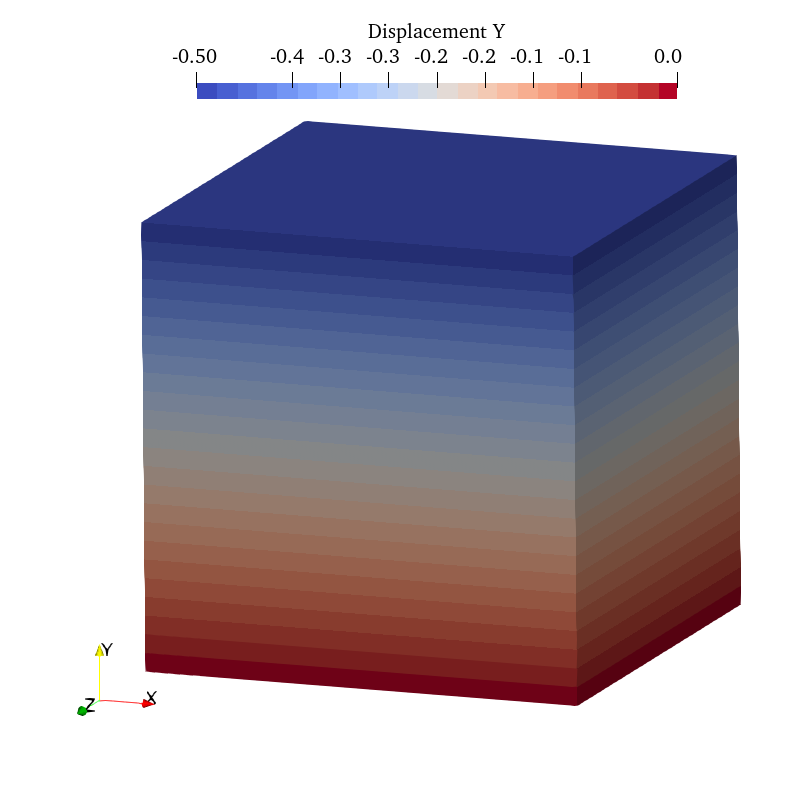
\includegraphics[width=0.4\textwidth,trim={1cm 1.5cm 1.5cm 0cm},clip]{non-homogeneous-stretch-dispy.png}} \qquad
    \subfloat[\label{fig:non-homogeneous-stretch-fields-b}]{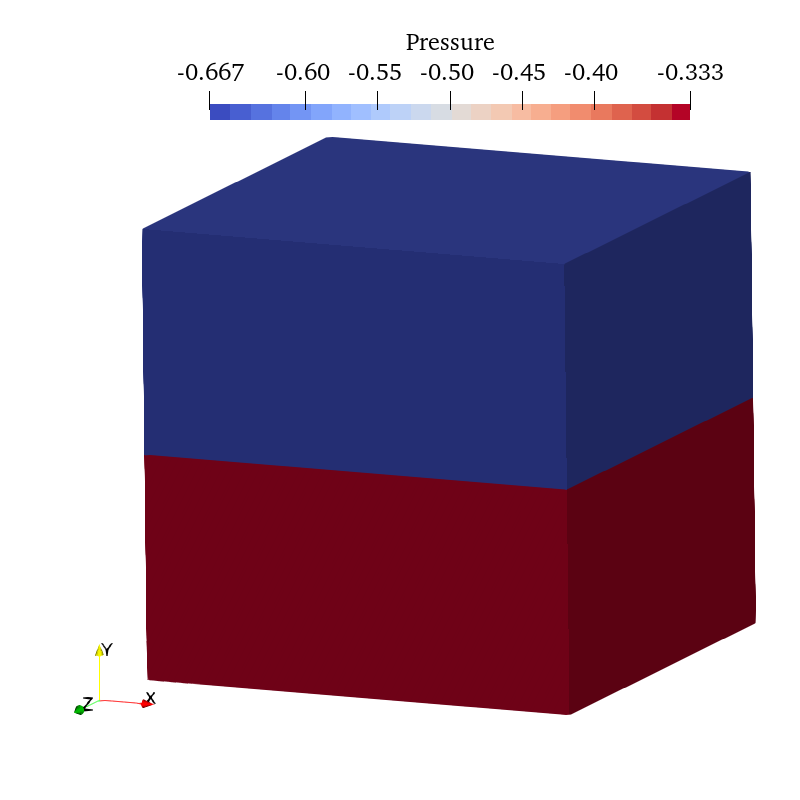
\includegraphics[width=0.4\textwidth,trim={1cm 1.5cm 1.5cm 0cm},clip]{non-homogeneous-stretch-pressure.png}} \\
    \subfloat[\label{fig:non-homogeneous-stretch-fields-c}]
    {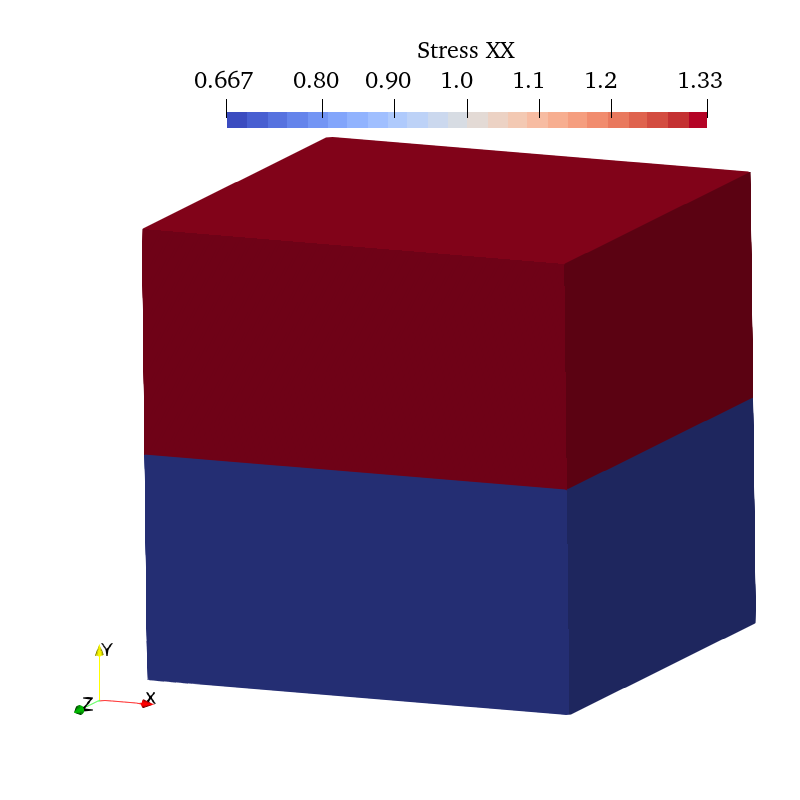
\includegraphics[width=0.4\textwidth,trim={1cm 1.5cm 1.5cm 0cm},clip]{non-homogeneous-stretch-stressxx.png}} \qquad
	\subfloat[\label{fig:non-homogeneous-stretch-fields-d}]
    {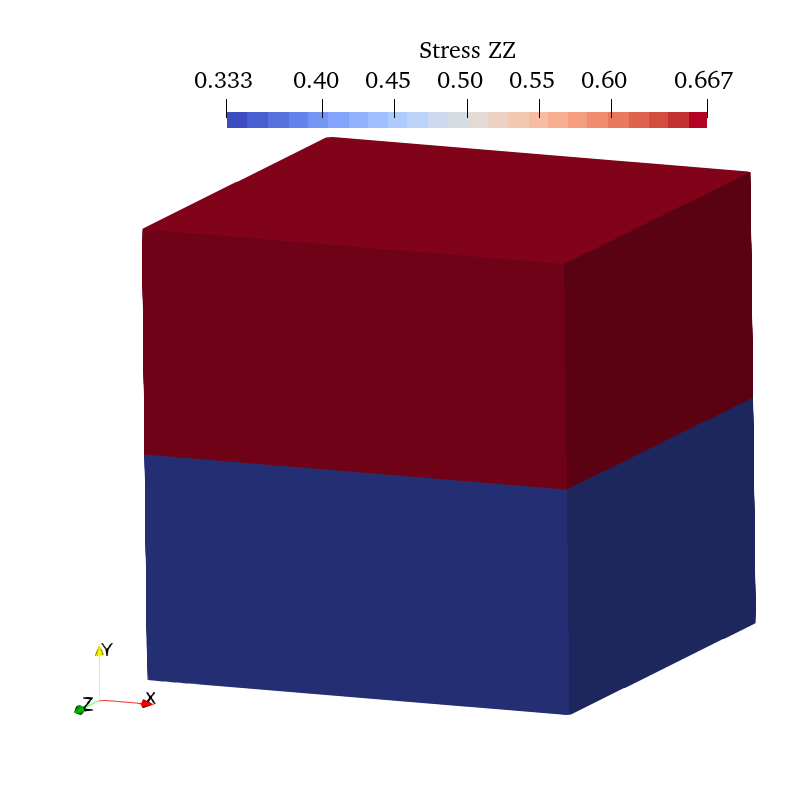
\includegraphics[width=0.4\textwidth,trim={1cm 1.5cm 1.5cm 0cm},clip]{non-homogeneous-stretch-stresszz.png}}
    \caption{Uniform stretch of a non-homogeneous material. (a) $u_y$, (b) $p$, (c) $\sigma_{xx}$ and (d) $\sigma_{zz}$ fields}
    \label{fig:non-homogeneous-stretch-fields}
\end{figure}

\subsection{Cantilever beam subjected to an end shear load \label{subsec:bishop}}

The case of a tridimensional cantilever beam under an end shear load is considered. Its initial geometry is depicted in Figure \ref{fig:bishop-beam-geometry}, with $L=5$, $a=0.5$, $b=0.5$. The beam is fixed at $z=0$ and is subjected to a downward shear force $F=1$ at $z=L$ in the $y$ direction. The other faces are traction-free. The material is assumed to have a linear isotropic behavior with a constant Young's modulus of $E=1$. To analyze the formulation across a broad range of material compressibility, different values of the Poisson ratio are considered.

\begin{figure}[H]
	\centering
	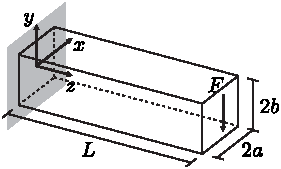
\includegraphics[scale=1.0]{bishop-beam-geometry}
	\caption{Cantilever beam subjected to an end shear load -- geometry.}
	\label{fig:bishop-beam-geometry}
\end{figure}

The analytical stress state for the problem is provided in \cite{bishop2014displacement} and is expressed as follows:
\begin{equation} \label{eq:bishop-stress}
	\begin{aligned}
		\sigma_{xx} &= \sigma_{xy} = \sigma_{yy} = 0 \text{,}\\
		\sigma_{zz} &= \frac{F}{I} yz \text{,}\\
		\sigma_{xz} &= \frac{F}{I} \frac{2a^2}{\pi^2}\frac{\nu}{1+\nu} \sum_{n=1}^{\infty} \frac{(-1)^n}{n^2} \text{sin}\left(n\pi x/a\right) \frac{\text{sinh}\left( n\pi y/a \right)}{\text{cosh}\left( n\pi b/a \right)} \text{,}\\
		\sigma_{yz} &= \frac{F}{I} \frac{b^2-y^2}{2} + \frac{F}{I}\frac{\nu}{1+\nu} \left[ \frac{3x^2-a^2}{6} - \frac{2a^2}{\pi^2} \sum_{n=1}^{\infty} \frac{(-1)^n}{n^2} \text{cos}\left(n\pi x/a\right) \frac{\text{cosh}\left( n\pi y/a \right)}{\text{cosh}\left( n\pi b/a \right)}  \right]\text{,}\\
	\end{aligned}
\end{equation}

\noindent where $F=\int_{-b}^{b}\int_{-a}^{a}\sigma_{yz}dxdy$ and $I=4ab^3/3$ is the second moment of area about the $x$-axis. The following displacement field is obtained by integrating Equations \eqref{eq:bishop-stress} and enforcing compatibility constraints:
\begin{equation} \label{eq:bishop-displacement}
	\begin{split}
		u_x & = -\frac{F\nu}{EI} xyz \text{,}\\
		u_y & = \frac{F}{EI} \left[ \frac{\nu}{2}\left(x^2-y^2\right)z - \frac{1}{6}z^3 \right] \text{,}\\
		u_z & = \frac{F}{EI} \left[ \frac{1}{2y}\left(\nu x^2+z^2\right)z + \frac{1}{6}\nu y^3 +(1+\nu) \left(b^2 y -\frac{1}{3}y^3\right) -\frac{1}{3}a^2 \nu y \right. \\
		&\qquad\quad \left.-\frac{4a^3\nu}{\pi^3} \sum_{n=1}^{\infty} \frac{(-1)^n}{n^3} \text{cos}\left(n\pi x/a\right) \frac{\text{sinh}\left( n\pi y/a \right)}{\text{cosh}\left( n\pi b/a \right)} \right] \text{.}
	\end{split}
\end{equation}

For the analyses that follow, we kept the number of terms in the series expansion limited to $n=5$. The exact solution evaluated on the boundaries of the beam is used to define the boundary conditions. At $z=0$, the exact normal and tangential displacements computed according to Eq. \eqref{eq:bishop-displacement} are prescribed, whereas surface tractions in accordance with Eq. \eqref{eq:bishop-stress} are applied on the other five faces.

Two types of mesh partitions are considered: one using tetrahedral elements and the other using hexahedral elements. For both cases, the average element size is computed as $h_e=1/2^{n-1}$, where $n=\{1,2,3,4,5\}$. The coarsest ($h_e=1$) and finest ($h_e=0.0625$) meshes for each partition are shown in Figure \ref{fig:bishop-meshes}. The first analysis is carried out keeping $\nu=0.3$ as in \cite{bishop2014displacement}. A convergence study is then performed, evaluating the $L^2$-norm errors for displacement, pressure, stress, and mass conservation.

\begin{figure}[H]
	\centering
	\subfloat[Hexahedral meshes. Coarsest (left) and finest (right).]{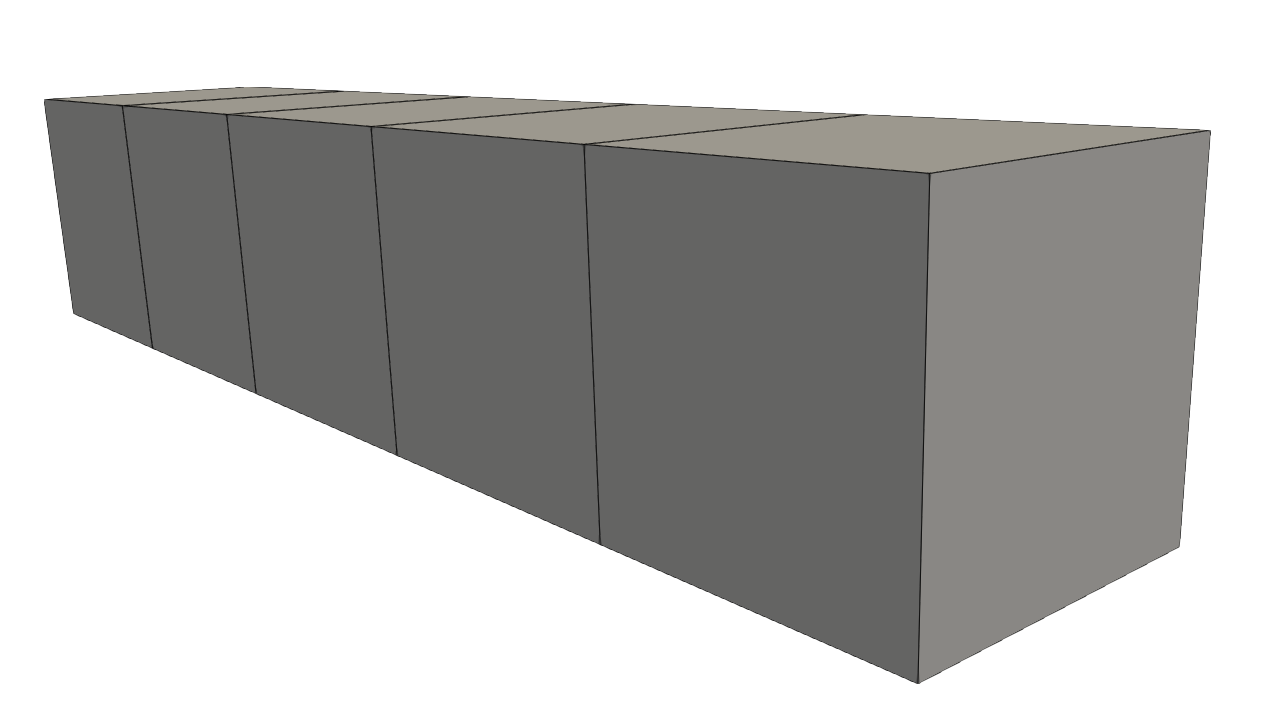
\includegraphics[width=0.48\textwidth]{bishop-mesh-hex-a.png}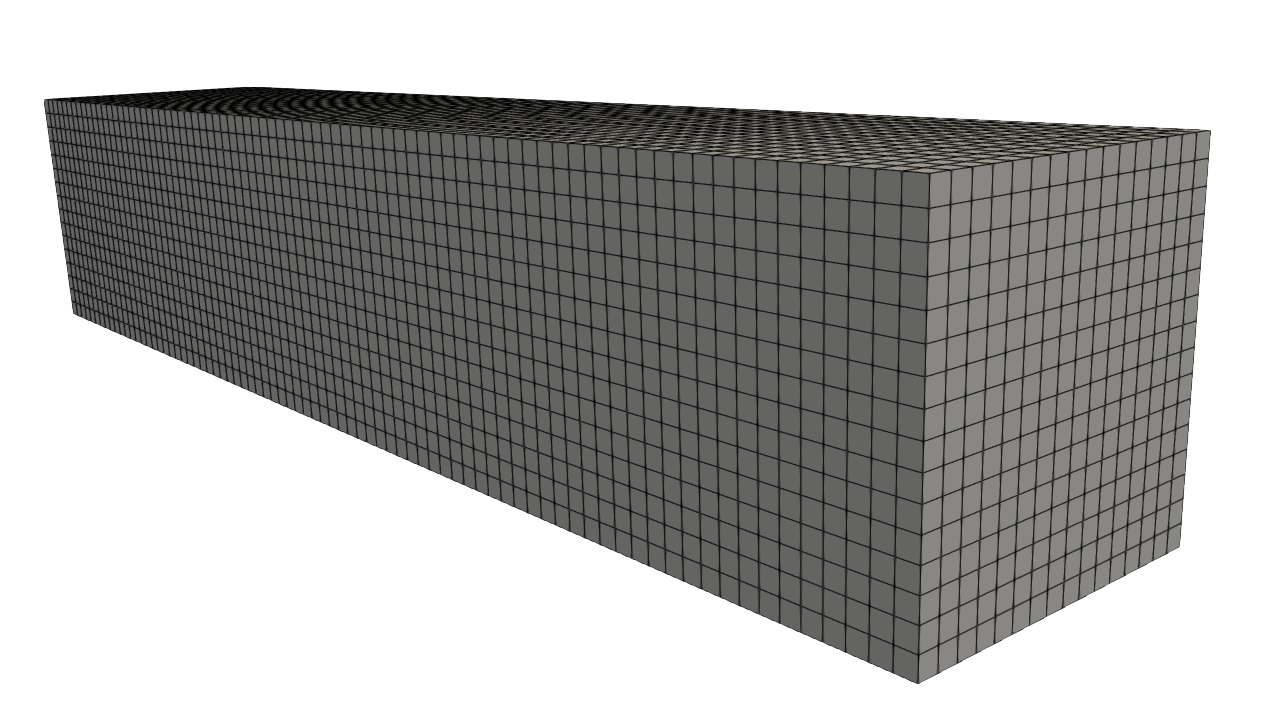
\includegraphics[width=0.48\textwidth]{bishop-mesh-hex-b.png}} \\
	\subfloat[Tetrahedral meshes. Coarsest (left) and finest (right).]{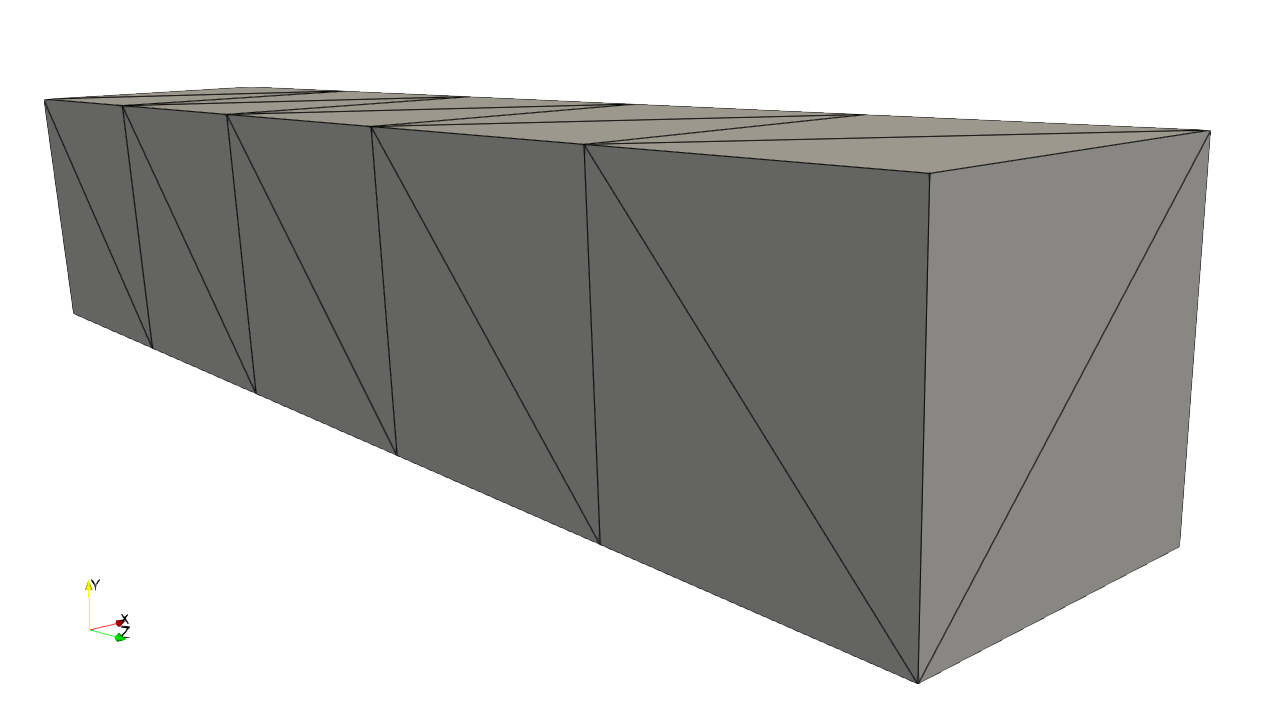
\includegraphics[width=0.48\textwidth]{bishop-mesh-tet-a.png}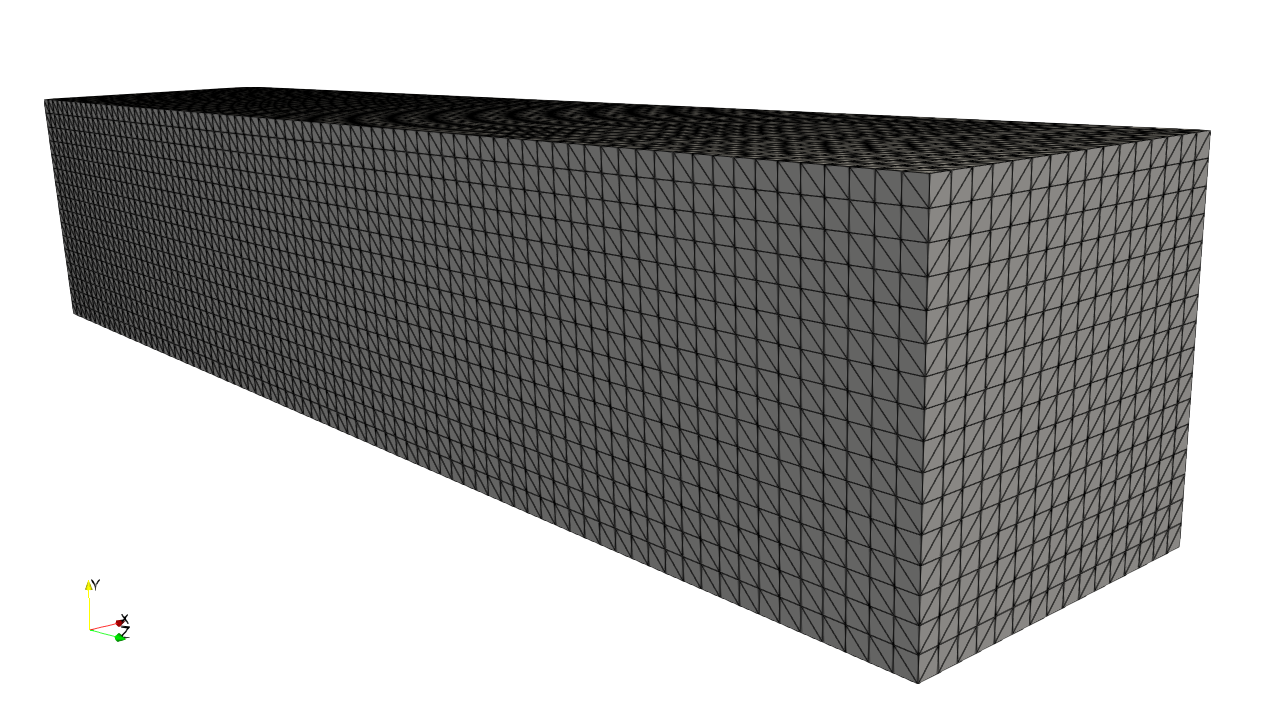
\includegraphics[width=0.48\textwidth]{bishop-mesh-tet-b.png}}
	\caption{Cantilever beam subjected to an end shear load. Meshes used for the convergence test}
	\label{fig:bishop-meshes}
\end{figure}

The results in Figure \ref{fig:bishop-convergence-nu-03} are similar using both mesh partitions, exhibiting optimal convergence rates of order $k+1$ for the displacement and $k$ for the other variables. Figure \ref{fig:bishop-snapshot} presents the displacement, pressure, stress magnitude, and Von Mises stress distributions obtained with the finest hexahedral mesh using $k=3$ over the deformed configuration beam. The results qualitatively agree with the reference solution \cite{bishop2014displacement}.

\begin{figure}[H]
    \centering
    \subfloat[\label{fig:bishop-convergence-nu-03-a}Displacement]{\includetikz{bishop-hex-disp-03}\includetikz{bishop-tet-disp-03}} \\
	\subfloat[\label{fig:bishop-convergence-nu-03-b}Pressure]{\includetikz{bishop-hex-pres-03}\includetikz{bishop-tet-pres-03}} \\
	\subfloat[\label{fig:bishop-convergence-nu-03-c}Stress]{\includetikz{bishop-hex-stress-03}\includetikz{bishop-tet-stress-03}} \\
	\subfloat[\label{fig:bishop-convergence-nu-03-d}Volumetric strain]{\includetikz{bishop-hex-div-03}\includetikz{bishop-tet-div-03}}
    \caption{Cantilever beam subjected to an end shear load. Convergence analysis for the compressible case ($\nu=0.3$) with hexahedral (at left) and tetrahedral (at right) elements using the DHM-H(div) formulation.}
    \label{fig:bishop-convergence-nu-03}
\end{figure}

\begin{figure}[H]
    \centering
    \subfloat[\label{fig:bishop-snapshot-a}Displacement]{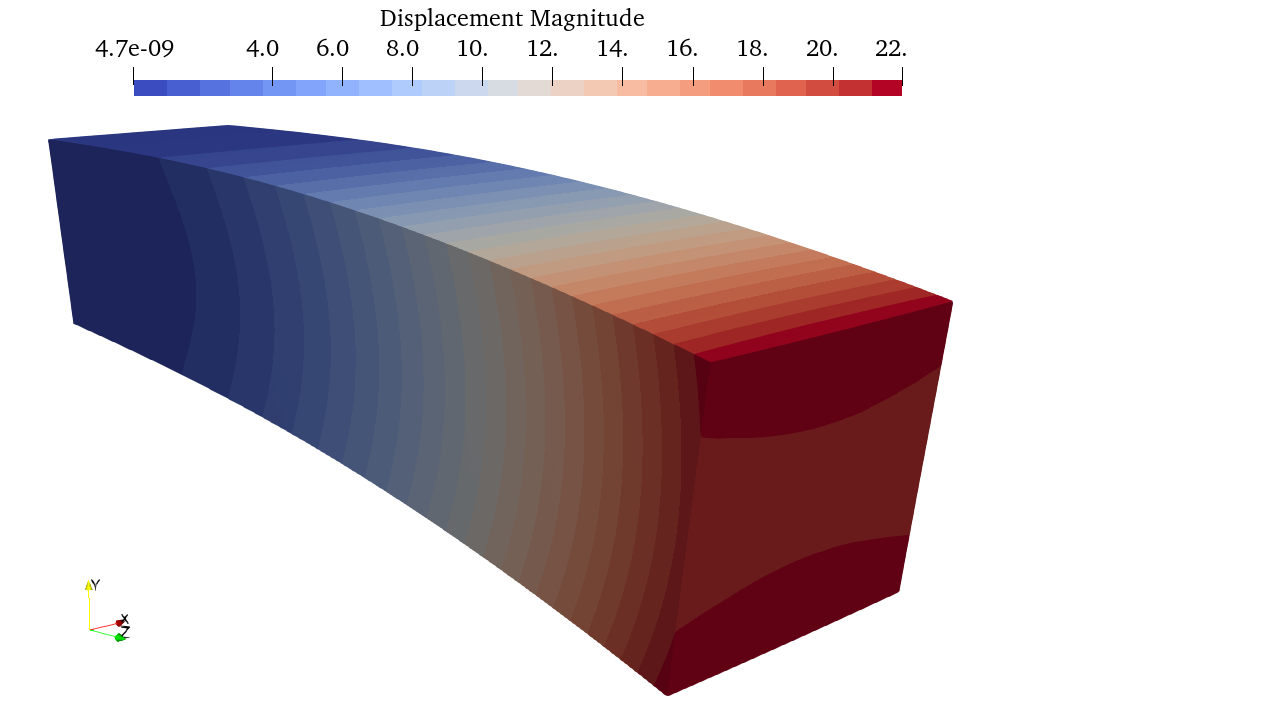
\includegraphics[width=0.47\textwidth,trim={0 0 8cm 0}, clip]{bishop-disp.png}} \hfill
    \subfloat[\label{fig:bishop-snapshot-b}Pressure]{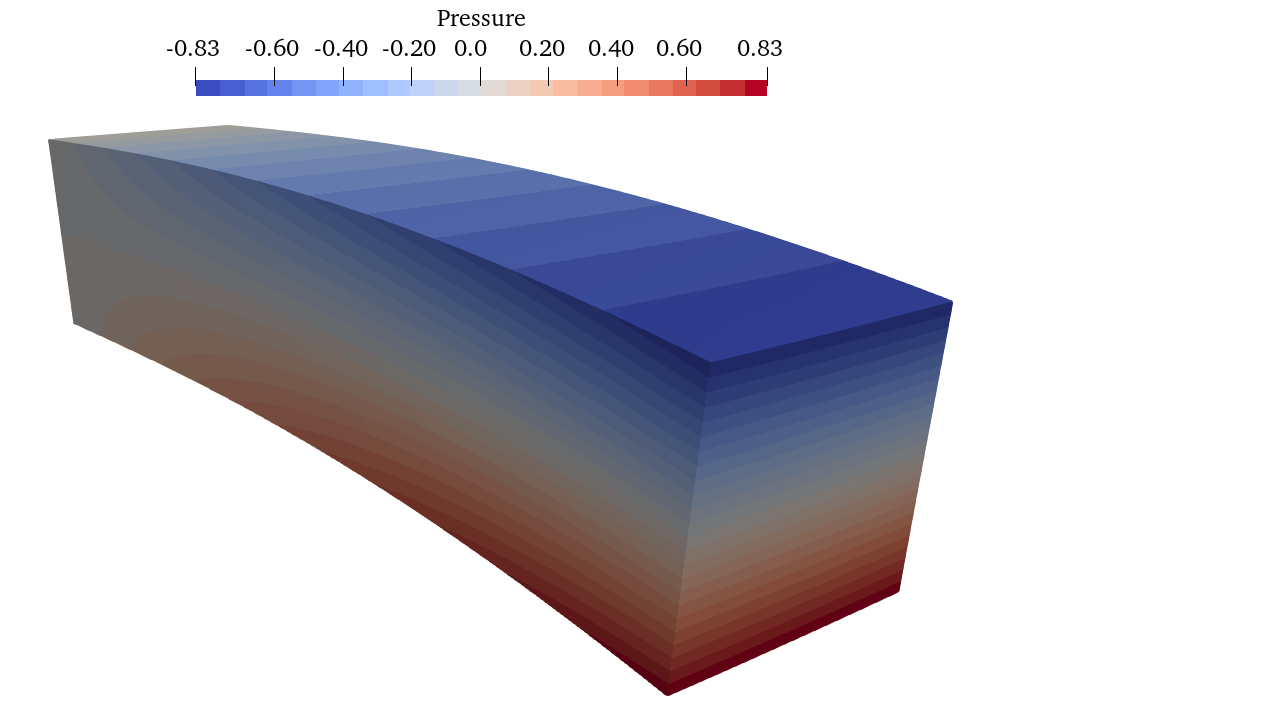
\includegraphics[width=0.47\textwidth,trim={0 0 8cm 0}, clip]{bishop-pressure.png}} \\
    \subfloat[\label{fig:bishop-snapshot-c}Stress magnitude]{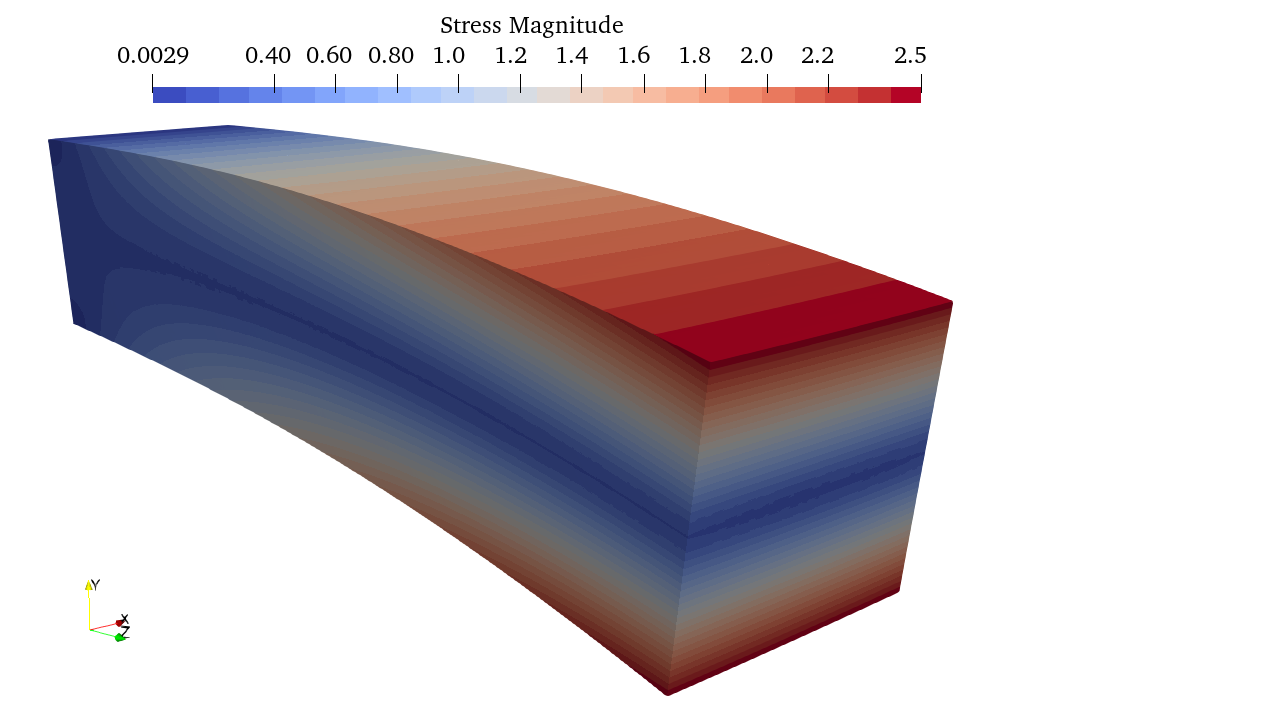
\includegraphics[width=0.47\textwidth,trim={0 0 8cm 0}, clip]{bishop-stress.png}} \hfill
    \subfloat[\label{fig:bishop-snapshot-d}Von Mises stress]{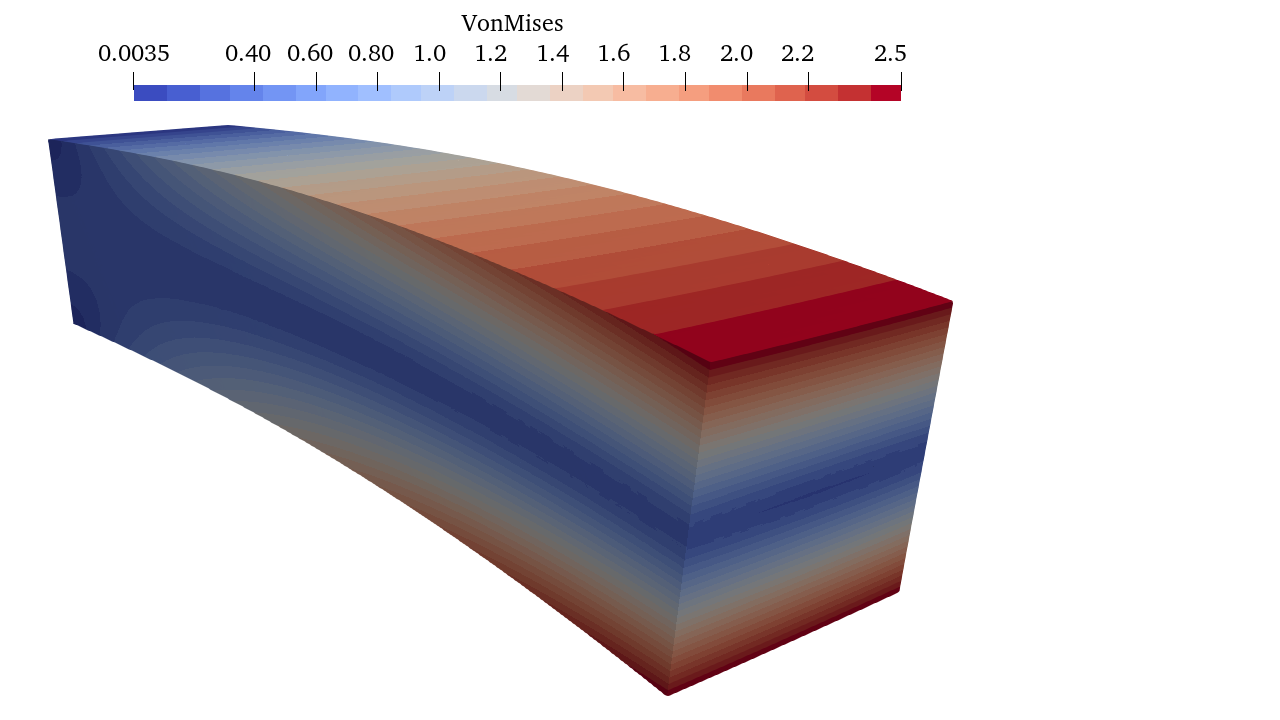
\includegraphics[width=0.47\textwidth,trim={0 0 8cm 0}, clip]{bishop-vonmises.png}}
    \caption{Cantilever beam subjected to an end shear load. Snapshots for $\nu=0.3$.}
    \label{fig:bishop-snapshot}
\end{figure}

To evaluate the proposed methodology across different compressibility regimes, Tables \ref{tab:bishop-convergence-049}-\ref{tab:bishop-convergence-050} present the convergence rates obtained for $\nu=0.49$, $\nu=0.4999$, and $\nu=0.5$. Optimal convergence rates are achieved independently of the Poisson ratio. This is a noteworthy feature, as many formulations suffer from locking under quasi and full incompressibility. Additionally, for the incompressible case ($\nu=0.5$), a divergence-free displacement field is obtained even for the coarsest mesh, with the error limited to machine precision.

\begin{table}[H]
    \centering
    \caption{Convergence rates for a cantilever beam under an end shear load with $\nu=0.49$. Results are shown for $\bm{u}$, $p$, $\bm{\sigma}$, and $\nabla \cdot \bm{u}$ using hexahedral (left) and tetrahedral (right) meshes with the DHM-H(div) formulation}
    \vspace{5pt}
	\resizebox{\textwidth}{!}{
    \begin{tabular}{c c c c c | c c c c}
        \toprule
        \multicolumn{5}{c}{\textbf{Hexahedral elements}} & \multicolumn{4}{c}{\textbf{Tetrahedral elements}} \\
        \cmidrule(r){1-5} \cmidrule(l){6-9}
        $h_e$ & $\|\bm{u} - \bm{u}_h\|$ & $\|p - p_h\|$ & $\|\boldsymbol{\sigma} - \boldsymbol{\sigma}_h\|$ & $\|\nabla \cdot (\bm{u} - \bm{u}_h)\|$ & $\|\bm{u} - \bm{u}_h\|$ & $\|p - p_h\|$ & $\|\boldsymbol{\sigma} - \boldsymbol{\sigma}_h\|$ & $\|\nabla \cdot (\bm{u} - \bm{u}_h)\|$ \\
        \midrule
        \multicolumn{9}{l}{$k = 1$} \\
		1       & $3.20E+00$ & $4.74E-01$ & $1.09E+00$ & $2.85E-02$ & $3.56E+00$ & $4.97E-01$ & $1.41E+00$ & $1.88E-02$ \\
		0.5     & $7.91E-01$ & $2.37E-01$ & $5.46E-01$ & $1.42E-02$ & $8.68E-01$ & $2.93E-01$ & $7.64E-01$ & $9.97E-03$ \\
		0.25    & $2.04E-01$ & $1.24E-01$ & $2.83E-01$ & $7.45E-03$ & $2.30E-01$ & $1.63E-01$ & $4.00E-01$ & $5.14E-03$ \\
		0.125   & $5.18E-02$ & $6.29E-02$ & $1.43E-01$ & $3.77E-03$ & $5.89E-02$ & $8.55E-02$ & $1.74E-01$ & $2.39E-03$ \\
		0.06125 & $1.30E-02$ & $3.16E-02$ & $7.18E-02$ & $1.89E-03$ & $1.51E-02$ & $4.09E-02$ & $7.91E-02$ & $1.08E-03$ \\
		Rate & $2.00$ & $1.00$ & $1.00$ & $1.00$ & $2.00$ & $1.00$ & $1.00$ & $1.00$ \\
		\midrule
		\multicolumn{9}{l}{$k = 2$} \\
		1       & $1.21E-01$ & $3.50E-02$ & $1.07E-01$ & $2.10E-03$ & $1.11E-01$ & $4.68E-02$ & $1.36E-01$ & $2.81E-03$ \\
		0.5     & $7.86E-03$ & $9.10E-03$ & $2.81E-02$ & $5.46E-04$ & $7.89E-03$ & $1.26E-02$ & $3.55E-02$ & $7.59E-04$ \\
		0.25    & $6.03E-04$ & $2.28E-03$ & $7.10E-03$ & $1.37E-04$ & $5.35E-04$ & $3.34E-03$ & $9.19E-03$ & $2.00E-04$ \\
		0.125   & $5.22E-05$ & $5.68E-04$ & $1.77E-03$ & $3.41E-05$ & $4.87E-05$ & $8.57E-04$ & $2.34E-03$ & $5.14E-05$ \\
		0.06125 & $5.05E-06$ & $1.42E-04$ & $4.43E-04$ & $8.50E-06$ & $5.35E-06$ & $2.17E-04$ & $5.88E-04$ & $1.30E-05$ \\
		Rate & $3.00$ & $2.00$ & $2.00$ & $2.00$ & $3.00$ & $2.00$ & $2.00$ & $2.00$ \\
		\midrule
		\multicolumn{9}{l}{$k = 3$} \\
		1       & $2.03E-03$ & $1.77E-03$ & $7.39E-03$ & $1.06E-04$ & $1.96E-03$ & $3.40E-03$ & $1.10E-02$ & $2.04E-04$ \\
		0.5     & $1.36E-04$ & $2.68E-04$ & $1.69E-03$ & $1.61E-05$ & $1.73E-04$ & $1.03E-03$ & $2.86E-03$ & $6.19E-05$ \\
		0.25    & $8.15E-06$ & $5.57E-05$ & $2.18E-04$ & $3.34E-06$ & $1.24E-05$ & $1.76E-04$ & $4.72E-04$ & $1.05E-05$ \\
		0.125   & $4.92E-07$ & $6.99E-06$ & $2.74E-05$ & $4.19E-07$ & $8.37E-07$ & $2.46E-05$ & $6.53E-05$ & $1.48E-06$ \\
		0.06125 & $1.14E-07$ & $8.67E-07$ & $3.41E-06$ & $5.20E-08$ & $5.21E-08$ & $2.74E-06$ & $7.26E-06$ & $1.64E-07$ \\
		Rate & $4.00$ & $3.00$ & $3.00$ & $3.00$ & $4.00$ & $3.00$ & $3.00$ & $3.00$ \\
        \bottomrule
    \end{tabular}}
	\label{tab:bishop-convergence-049}
\end{table}

\begin{table}[H]
    \centering
    \caption{Convergence rates for a cantilever beam under an end shear load with $\nu=0.4999$. Results are presented for $\bm{u}$, $p$, $\bm{\sigma}$ and $\nabla \cdot \bm{u}$ using hexahedral (left) and tetrahedral (right) meshes with the DHM-H(div) formulation}
    \vspace{5pt}
	\resizebox{\textwidth}{!}{
    \begin{tabular}{c c c c c | c c c c}
        \toprule
        \multicolumn{5}{c}{\textbf{Hexahedral elements}} & \multicolumn{4}{c}{\textbf{Tetrahedral elements}} \\
        \cmidrule(r){1-5} \cmidrule(l){6-9}
        $h_e$ & $\|\bm{u} - \bm{u}_h\|$ & $\|p - p_h\|$ & $\|\boldsymbol{\sigma} - \boldsymbol{\sigma}_h\|$ & $\|\nabla \cdot (\bm{u} - \bm{u}_h)\|$ & $\|\bm{u} - \bm{u}_h\|$ & $\|p - p_h\|$ & $\|\boldsymbol{\sigma} - \boldsymbol{\sigma}_h\|$ & $\|\nabla \cdot (\bm{u} - \bm{u}_h)\|$ \\
        \midrule
        \multicolumn{9}{l}{$k = 1$} \\
		1       & $3.23E+00$ & $4.86E-01$ & $1.11E+00$ & $2.91E-04$ & $3.02E+00$ & $5.68E-01$ & $1.15E+00$ & $2.02E-04$ \\
		0.5     & $8.07E-01$ & $2.43E-01$ & $5.57E-01$ & $1.46E-04$ & $8.63E-01$ & $3.34E-01$ & $6.25E-01$ & $1.12E-04$ \\
		0.25    & $2.09E-01$ & $1.27E-01$ & $2.89E-01$ & $7.63E-05$ & $2.33E-01$ & $1.81E-01$ & $3.11E-01$ & $5.85E-05$ \\
		0.125   & $5.29E-02$ & $6.45E-02$ & $1.46E-01$ & $3.87E-05$ & $5.98E-02$ & $5.75E-02$ & $1.49E-01$ & $2.92E-05$ \\
		0.06125 & $1.33E-02$ & $3.24E-02$ & $7.34E-02$ & $1.94E-05$ & $1.44E-02$ & $2.92E-02$ & $7.70E-02$ & $1.36E-05$ \\
		Rate & $2.00$ & $1.00$ & $1.00$ & $1.00$ & $2.00$ & $1.00$ & $1.00$ & $1.00$ \\
		\midrule
		\multicolumn{9}{l}{$k = 2$} \\
		1       & $1.23E-01$ & $3.58E-02$ & $1.08E-01$ & $2.15E-05$ & $1.11E-01$ & $4.78E-02$ & $1.37E-01$ & $2.87E-05$ \\
		0.5     & $7.94E-03$ & $9.31E-03$ & $2.84E-02$ & $5.59E-06$ & $7.90E-03$ & $1.30E-02$ & $3.60E-02$ & $7.78E-06$ \\
		0.25    & $6.09E-04$ & $2.33E-03$ & $7.19E-03$ & $1.40E-06$ & $5.38E-04$ & $3.43E-03$ & $9.33E-03$ & $2.06E-06$ \\
		0.125   & $5.30E-05$ & $5.81E-04$ & $1.80E-03$ & $3.49E-07$ & $4.91E-05$ & $8.81E-04$ & $2.38E-03$ & $5.29E-07$ \\
		0.06125 & $5.14E-06$ & $1.45E-04$ & $4.49E-04$ & $8.69E-08$ & $5.41E-06$ & $2.23E-04$ & $5.99E-04$ & $1.34E-07$ \\
		Rate & $3.00$ & $2.00$ & $2.00$ & $2.00$ & $3.00$ & $2.00$ & $2.00$ & $2.00$ \\
		\midrule
		\multicolumn{9}{l}{$k = 3$} \\
		1       & $2.09E-03$ & $1.84E-03$ & $7.55E-03$ & $1.10E-06$ & $2.04E-03$ & $3.56E-03$ & $1.13E-02$ & $2.14E-06$ \\
		0.5     & $1.38E-04$ & $2.79E-04$ & $1.72E-03$ & $1.67E-07$ & $1.77E-04$ & $1.08E-03$ & $2.94E-03$ & $2.46E-07$ \\
		0.25    & $8.36E-06$ & $5.80E-05$ & $2.23E-04$ & $3.48E-08$ & $1.27E-05$ & $1.83E-04$ & $4.87E-04$ & $2.87E-08$ \\
		0.125   & $5.04E-07$ & $7.29E-06$ & $2.81E-05$ & $4.37E-09$ & $8.56E-07$ & $2.57E-05$ & $6.74E-05$ & $3.54E-09$ \\
		0.06125 & $1.21E-07$ & $9.04E-07$ & $3.49E-06$ & $5.44E-10$ & $5.46E-08$ & $2.86E-06$ & $7.50E-06$ & $3.99E-10$ \\
		Rate & $4.00$ & $3.00$ & $3.00$ & $3.00$ & $4.00$ & $3.00$ & $3.00$ & $3.00$ \\
        \bottomrule
    \end{tabular}}
	\label{tab:bishop-convergence-04999}
\end{table}

\begin{table}[H]
    \centering
    \caption{Convergence rates for a cantilever beam under an end shear load with $\nu=0.5$. Results are presented for $\bm{u}$, $p$, $\bm{\sigma}$ and $\nabla \cdot \bm{u}$ using hexahedral (left) and tetrahedral (right) meshes with the DHM-H(div) formulation}
    \vspace{5pt}
	\resizebox{\textwidth}{!}{
    \begin{tabular}{c c c c c | c c c c}
        \toprule
        \multicolumn{5}{c}{\textbf{Hexahedral elements}} & \multicolumn{4}{c}{\textbf{Tetrahedral elements}} \\
        \cmidrule(r){1-5} \cmidrule(l){6-9}
        $h_e$ & $\|\bm{u} - \bm{u}_h\|$ & $\|p - p_h\|$ & $\|\boldsymbol{\sigma} - \boldsymbol{\sigma}_h\|$ & $\|\nabla \cdot (\bm{u} - \bm{u}_h)\|$ & $\|\bm{u} - \bm{u}_h\|$ & $\|p - p_h\|$ & $\|\boldsymbol{\sigma} - \boldsymbol{\sigma}_h\|$ & $\|\nabla \cdot (\bm{u} - \bm{u}_h)\|$ \\
        \midrule
        \multicolumn{9}{l}{$k = 1$} \\
        1       & $3.28E+00$ & $4.86E-01$ & $1.11E+00$ & $2.34E-13$ & $3.72E+00$ & $5.18E-01$ & $1.25E+00$ & $2.76E-13$ \\
        0.5     & $8.07E-01$ & $2.43E-01$ & $5.57E-01$ & $3.57E-13$ & $9.39E-01$ & $2.39E-01$ & $6.25E-01$ & $4.52E-13$ \\
        0.25    & $2.02E-01$ & $1.21E-01$ & $2.78E-01$ & $4.65E-13$ & $2.25E-01$ & $1.27E-01$ & $3.11E-01$ & $4.76E-13$ \\
        0.125   & $5.04E-02$ & $6.07E-02$ & $1.39E-01$ & $7.05E-13$ & $5.87E-02$ & $6.44E-02$ & $1.49E-01$ & $4.61E-13$ \\
        0.06125 & $1.26E-02$ & $3.04E-02$ & $6.96E-02$ & $8.03E-13$ & $1.43E-02$ & $3.21E-02$ & $7.69E-02$ & $6.88E-13$ \\
        Rate & $2.00$ & $1.00$ & $1.00$ & --- & $2.00$ & $1.00$ & $1.00$ & --- \\
        \midrule
		\multicolumn{9}{l}{$k = 2$} \\
		1       & $1.23E-01$ & $3.58E-02$ & $1.08E-01$ & $4.58E-12$ & $1.11E-01$ & $4.78E-02$ & $1.37E-01$ & $1.17E-12$ \\
		0.5     & $7.61E-03$ & $9.32E-03$ & $2.82E-02$ & $1.01E-11$ & $7.90E-03$ & $1.30E-02$ & $3.60E-02$ & $2.00E-12$ \\
		0.25    & $5.35E-04$ & $2.37E-03$ & $7.28E-03$ & $1.95E-11$ & $5.38E-04$ & $3.43E-03$ & $9.33E-03$ & $3.86E-12$ \\
		0.125   & $4.84E-05$ & $5.96E-04$ & $1.87E-03$ & $3.89E-11$ & $4.91E-05$ & $8.81E-04$ & $2.38E-03$ & $7.74E-12$ \\
		0.06125 & $4.99E-06$ & $1.49E-04$ & $4.69E-04$ & $7.94E-11$ & $5.37E-06$ & $2.23E-04$ & $5.99E-04$ & $1.57E-11$ \\
		Rate & $3.00$ & $2.00$ & $2.00$ & --- & $3.00$ & $2.00$ & $2.00$ & --- \\
		\midrule
		\multicolumn{9}{l}{$k = 3$} \\
		1       & $2.09E-03$ & $1.84E-03$ & $7.55E-03$ & $2.17E-12$ & $2.04E-03$ & $3.56E-03$ & $1.13E-02$ & $4.27E-12$ \\
		0.5     & $1.38E-04$ & $2.79E-04$ & $1.72E-03$ & $4.58E-12$ & $1.77E-04$ & $1.08E-03$ & $2.94E-03$ & $7.30E-12$ \\
		0.25    & $8.36E-06$ & $5.81E-05$ & $2.23E-04$ & $7.97E-12$ & $1.27E-05$ & $1.83E-04$ & $4.87E-04$ & $1.42E-11$ \\
		0.125   & $5.40E-07$ & $7.29E-06$ & $2.81E-05$ & $1.69E-11$ & $8.46E-07$ & $2.57E-05$ & $6.74E-05$ & $2.81E-11$ \\
		0.06125 & $3.40E-08$ & $9.04E-07$ & $3.49E-06$ & $3.50E-11$ & $5.44E-08$ & $2.89E-06$ & $7.58E-06$ & $3.27E-11$ \\
		Rate & $4.00$ & $3.00$ & $3.00$ & --- & $4.00$ & $3.00$ & $3.00$ & --- \\
        \bottomrule
    \end{tabular}}
	\label{tab:bishop-convergence-050}
\end{table}

We compare the error as a function of the number of degrees of freedom in the global system against the Taylor-Hood formulation for $\nu=0.5$. According to Figure \ref{fig:bishop-comparison-TH}, the DHM-H(div) formulation demonstrates competitive performance, showing a similar convergence rate compared to the Taylor-Hood elements using both partitions. The most significant difference appears in the pressure error, where the results using Taylor-Hood elements indicate a superconvergent rate. This behavior can be attributed to the pressure analytic solution being already included in the approximation space, a phenomenon also reported in \cite{puga2025stable} for a Stokes flow problem. Nonetheless, the DHM-H(div) formulation exactly represent the volumetric strain independently of the number of degrees of freedom, being advantageous for fully incompressible materials.
\begin{figure}[H]
    \centering
	\includetikz{TH-bishop-legend} \\
    \subfloat[\label{fig:bishop-comparison-TH-a}Displacement]{\includetikz{TH-bishop-hex-disp-05}\includetikz{TH-bishop-tet-disp-05}} \\
	\subfloat[\label{fig:bishop-comparison-TH-b}Pressure]{\includetikz{TH-bishop-hex-pres-05}\includetikz{TH-bishop-tet-pres-05}} \\
	\subfloat[\label{fig:bishop-comparison-TH-c}Stress]{\includetikz{TH-bishop-hex-stress-05}\includetikz{TH-bishop-tet-stress-05}} \\
	\subfloat[\label{fig:bishop-comparison-TH-d}Volumetric strain]{\includetikz{TH-bishop-hex-div-05}\includetikz{TH-bishop-tet-div-05}}
    \caption{Cantilever beam subjected to an end shear load. Error analysis with respect to the number of degrees of freedom for $\nu=0.5$ with hexahedral (left) and tetrahedral (right) elements using the DHM-H(div) and Taylor-Hood formulations.}
    \label{fig:bishop-comparison-TH}
\end{figure}

\subsection{Cook's membrane \label{subsec:cook}}

The Cook's membrane is a classical benchmark for evaluating locking phenomena of incompressible and nearly incompressible elasticity problems under shear and bending. It consists of a tapered cantilever beam, clamped at its left side and subjected to a shear load of $F=6.25$ N/mm in the $y$ direction at $x=48$ mm, as illustrated in Figure \ref{fig:cooks-geometry}. The material is assumed to have a linear behavior with a constant Young's modulus $E=240.565$ MPa and two different Poisson ratios are tested, according to the references: $\nu=0.4999$ and $\nu=0.4999999$. This problem is found in many books and papers, such as in \cite{cook1989concepts,elguedj2008b,cesar1999new}, with different material properties, geometries, and boundary conditions. Some studies have investigated this problem in the context of large displacements and strains, considering both elastic and elastoplastic materials \cite{chavan2007locking,elguedj2008b,de1996design}. In this work, we focus exclusively on linear elastic analysis.

\begin{figure}[H]
    \centering
    \input{cooks-membrane.pdf_tex}
    \caption{Cook's membrane -- geometry.}
    \label{fig:cooks-geometry}
\end{figure}

At first, we perform plane strain analyses using structured meshes with triangular and quadrilateral partitions, refined uniformly. The number of elements per edge adopted is $N_e=2^n$, with $n={0,1,2,3,4,5}$. Some of the meshes employed are shown in Figures \ref{fig:cooks-2d-tri-meshes}-\ref{fig:cooks-2d-quad-meshes}.

\begin{figure}[H]
	\centering
	\subfloat[$N_e=1$]{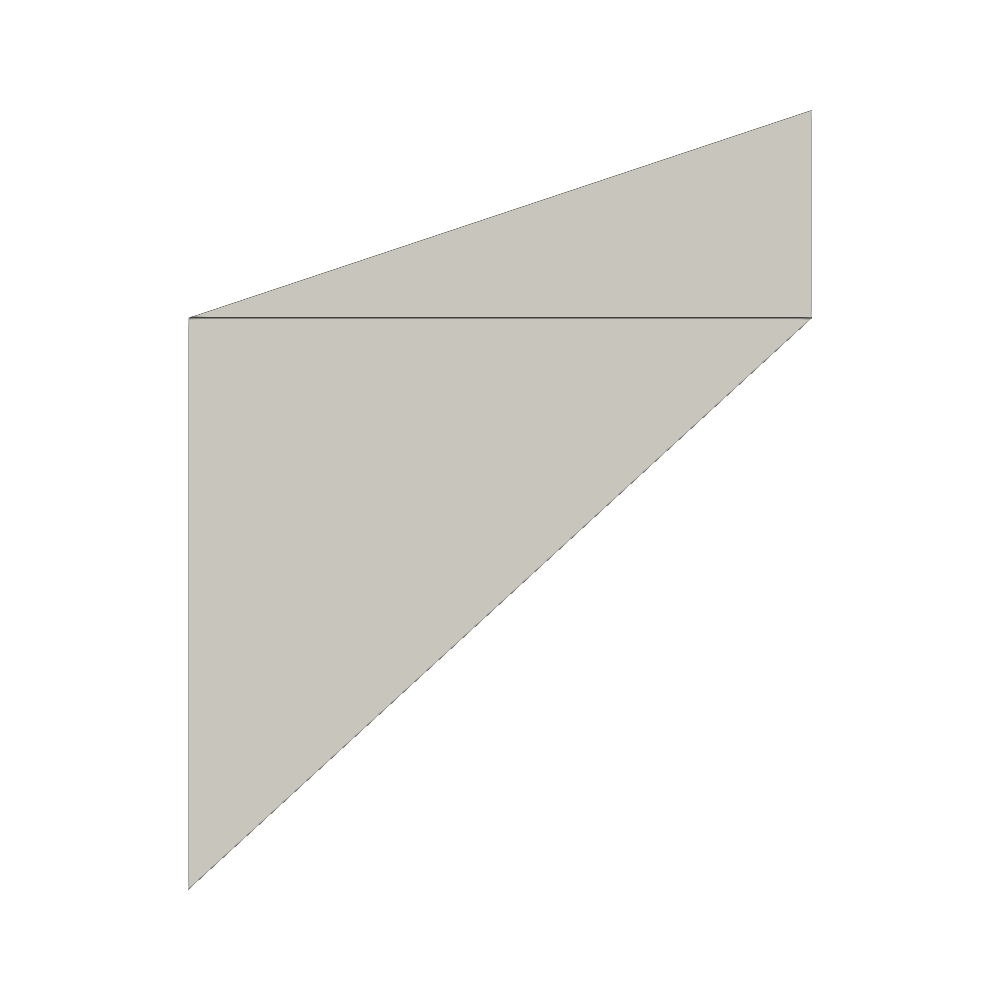
\includegraphics[width=0.25\textwidth, trim={4cm 4cm 4cm 3.5cm}, clip]{cooks-2d-tri-mesh-1.png}}
	\subfloat[$N_e=2$]{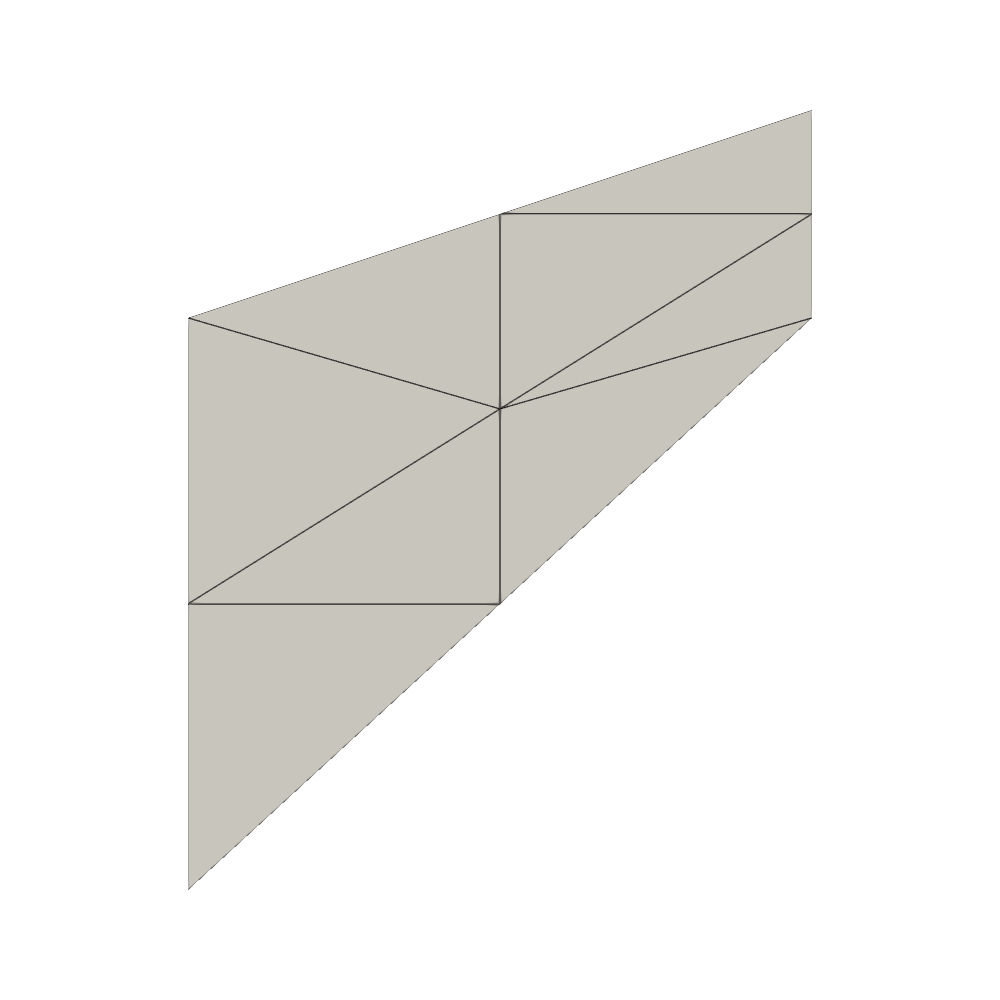
\includegraphics[width=0.25\textwidth, trim={4cm 4cm 4cm 3.5cm}, clip]{cooks-2d-tri-mesh-2.png}}
	\subfloat[$N_e=8$]{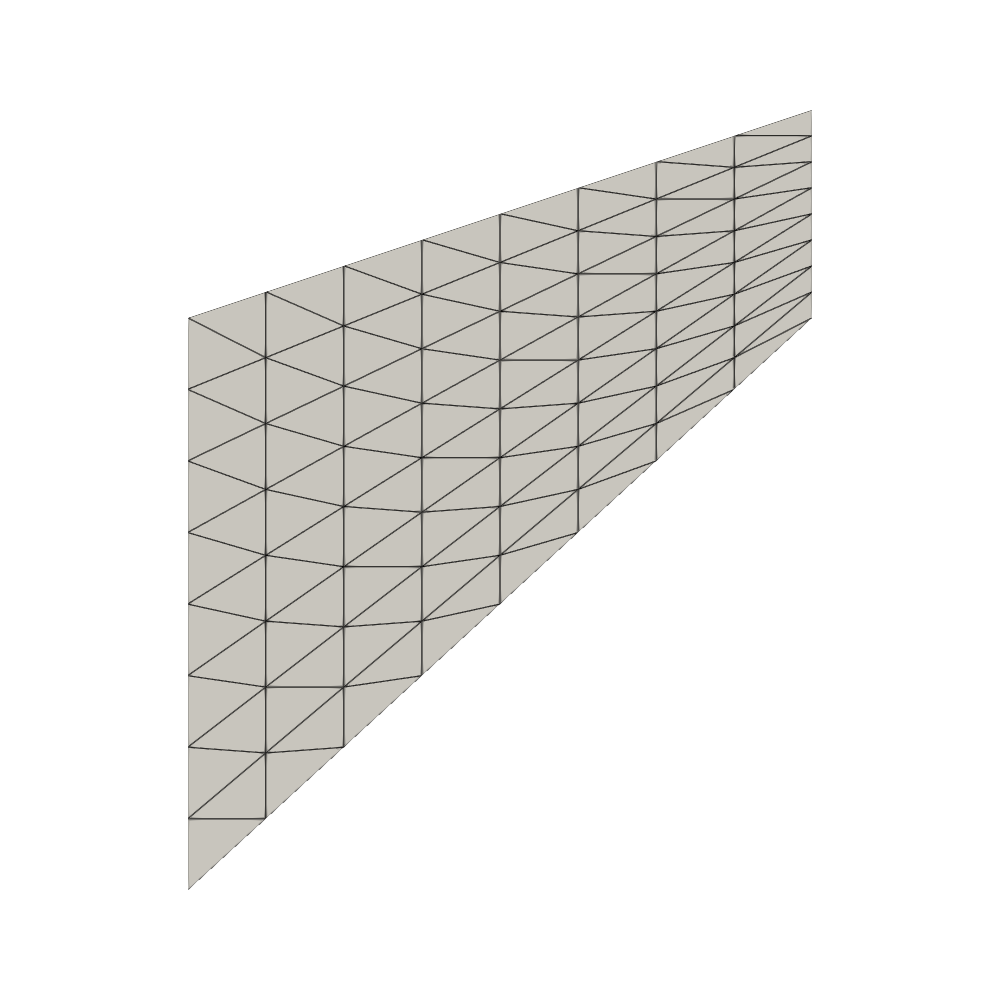
\includegraphics[width=0.25\textwidth, trim={4cm 4cm 4cm 3.5cm}, clip]{cooks-2d-tri-mesh-8.png}}
	\subfloat[$N_e=32$]{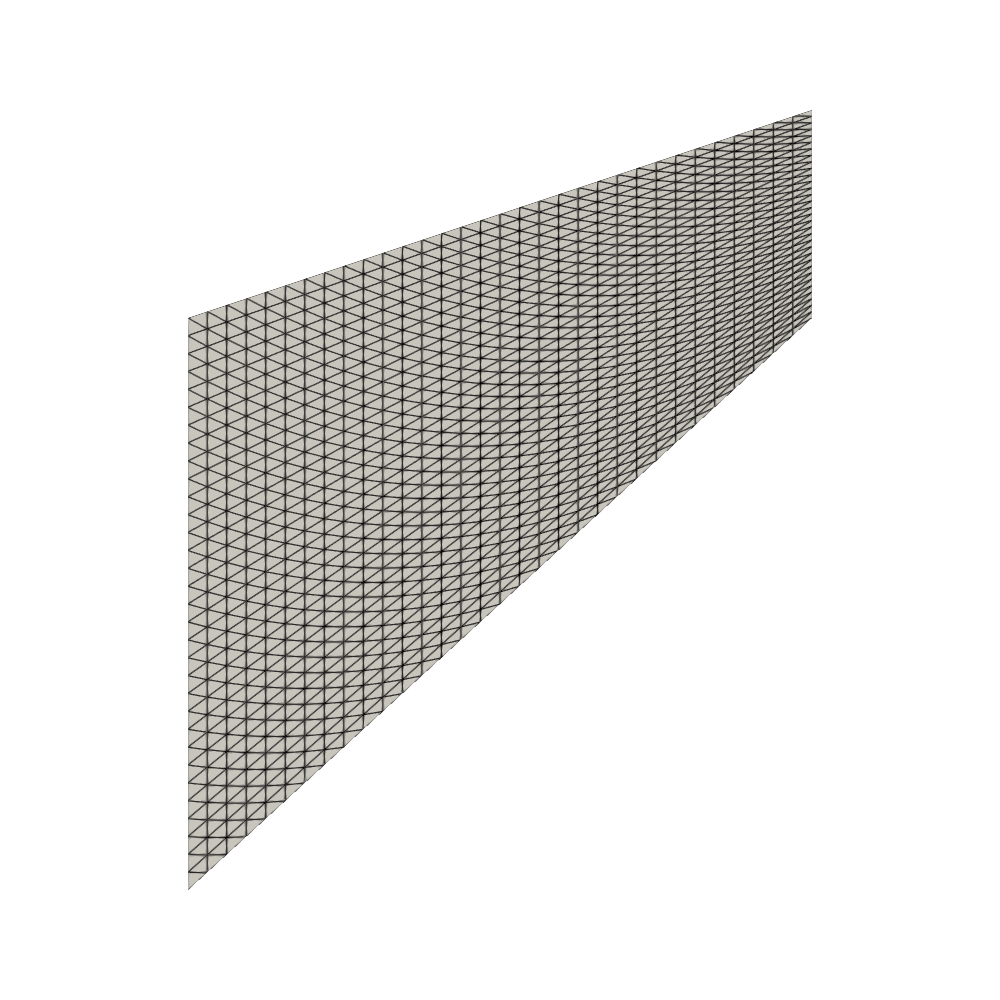
\includegraphics[width=0.25\textwidth, trim={4cm 4cm 4cm 3.5cm}, clip]{cooks-2d-tri-mesh-32.png}}
	\caption{Cook's membrane. Plane strain meshes with triangular partitions.}
	\label{fig:cooks-2d-tri-meshes}
\end{figure}

\begin{figure}[H]
	\centering
	\subfloat[$N_e=1$]{
\includegraphics[width=0.25\textwidth, trim={4cm 4cm 4cm 3.5cm}, clip]{cooks-2d-quad-mesh-1.png}} \hfill
	\subfloat[$N_e=2$]{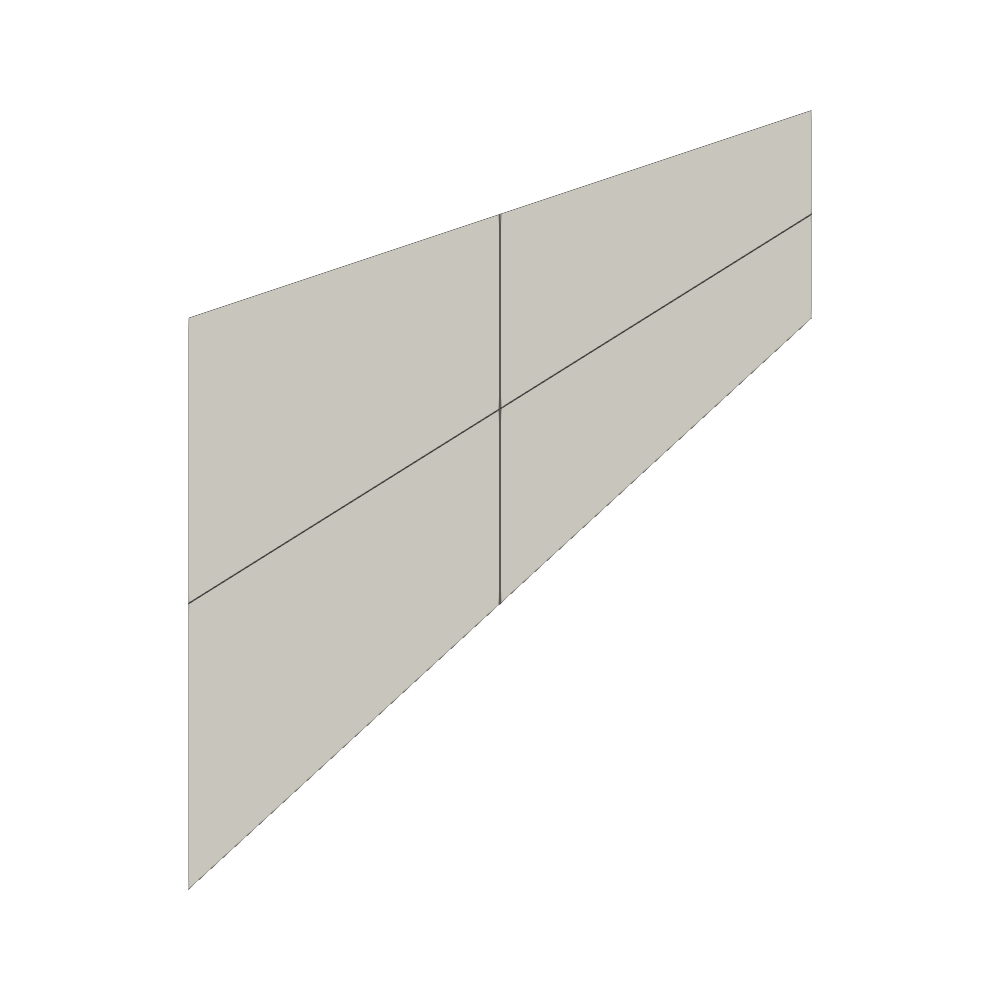
\includegraphics[width=0.25\textwidth, trim={4cm 4cm 4cm 3.5cm}, clip]{cooks-2d-quad-mesh-2.png}} \hfill
	\subfloat[$N_e=8$]{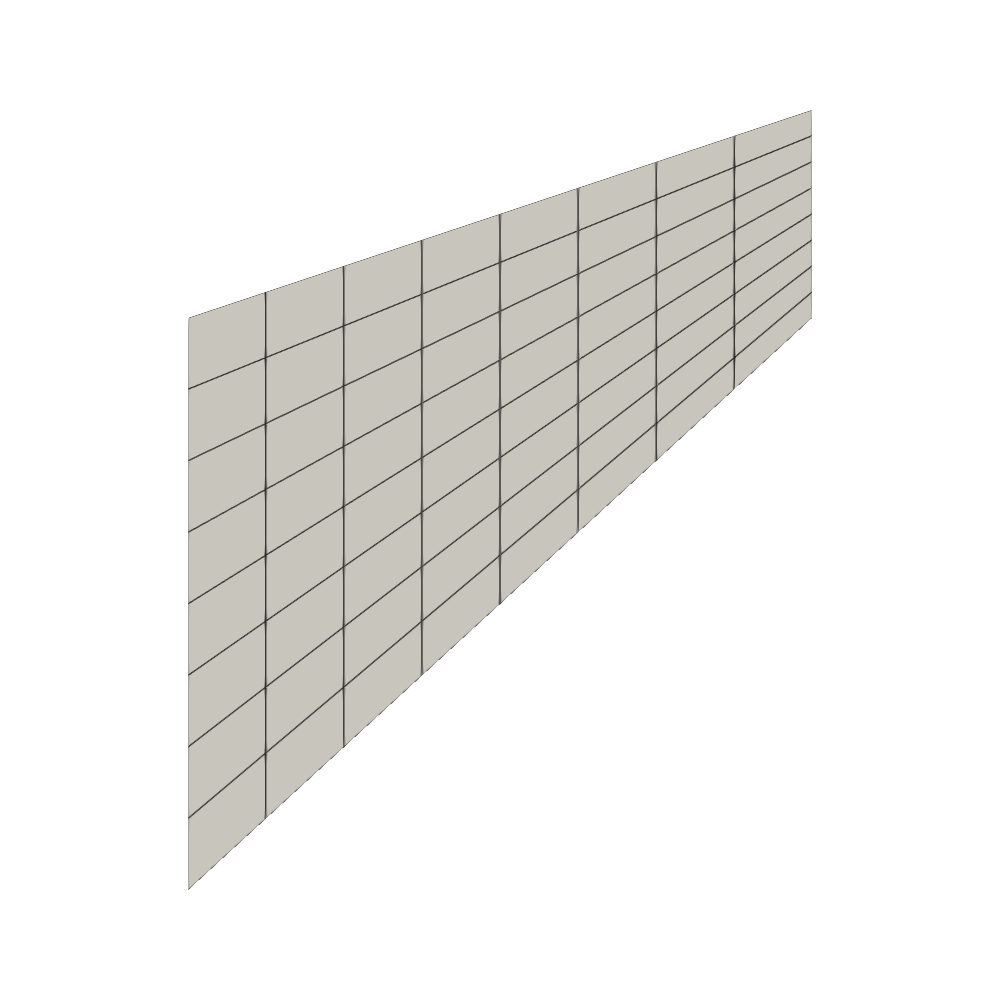
\includegraphics[width=0.25\textwidth, trim={4cm 4cm 4cm 3.5cm}, clip]{cooks-2d-quad-mesh-8.png}} \hfill
	\subfloat[$N_e=32$]{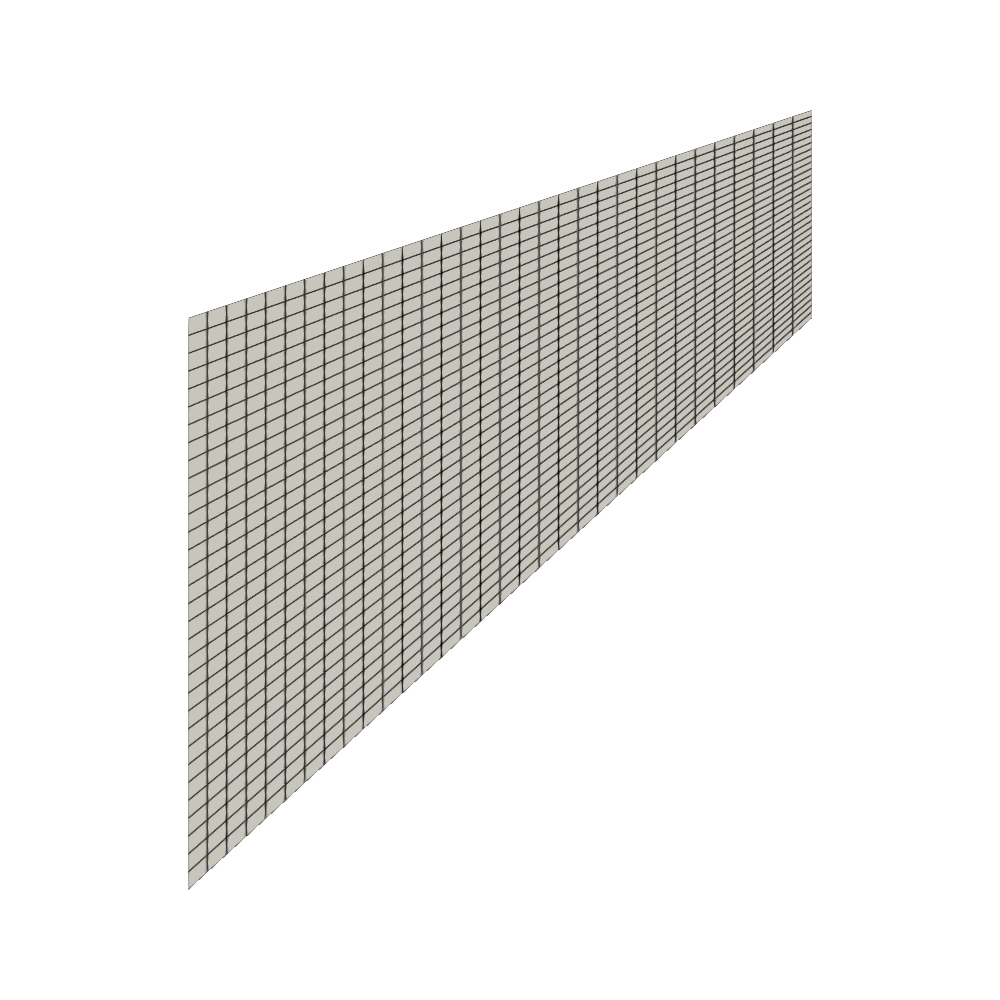
\includegraphics[width=0.25\textwidth, trim={4cm 4cm 4cm 3.5cm}, clip]{cooks-2d-quad-mesh-32.png}}
	\caption{Cook's membrane. Plane strain meshes with quadrilateral partitions.}
	\label{fig:cooks-2d-quad-meshes}
\end{figure}

Figure \ref{fig:cooks-2d-displacement-nu-0.4999} shows a comparison of the vertical displacement of point A for two values of $\nu$, alongside numerical results available in the literature \cite{elguedj2008b,cesar1999new} and results obtained using Taylor-Hood elements $P_kP_{k-1}$ with $k=\{2,3,4\}$. The DHM-H(div) formulation leads to a locking-free solution even for lower-order approximations ($k=1$), and qualitatively matches the reference solutions for both values of $\nu$ and mesh partitions. Moreover, the solution is practically the same for both values of $\nu$.
\begin{figure}[H]
    \centering
	\includetikz{cook-2d-disp-legend-04999} \\
    \subfloat[\label{fig:cooks-2d-displacement-nu-0.4999-a}]{\includetikz{cook-2d-quad-disp-04999}} \hfill
	\subfloat[\label{fig:cooks-2d-displacement-nu-0.4999-b}]{\includetikz{cook-2d-tri-disp-04999}}
    \caption{Cook's membrane. Vertical displacement of point A for $\nu=0.4999$ using (a) quadrilateral and (b) triangular partitions.}
    \label{fig:cooks-2d-displacement-nu-0.4999}
\end{figure}
\begin{figure}[H]
    \centering
	\includetikz{cook-2d-disp-legend-04999999} \\
    \subfloat[\label{fig:cooks-2d-displacement-nu-0.4999999-a}]{\includetikz{cook-2d-quad-disp-04999999}} \hfill
	\subfloat[\label{fig:cooks-2d-displacement-nu-0.4999999-b}]{\includetikz{cook-2d-tri-disp-04999999}}
    \caption{Cook's membrane. Vertical displacement of point A for $\nu=0.4999999$ using (a) quadrilateral and (b) triangular partitions.}
    \label{fig:cooks-2d-displacement-nu-0.4999999}
\end{figure}

The three-dimensional case is studied using similar meshes with hexahedra and tetrahedra elements for $\nu=0.5$. Zero normal displacement is imposed at the facets parallel to the $x-y$ plane to simulate a plane strain condition. Table \ref{tab:cooks-3d} shows the displacement obtained with the different partitions and polynomial degrees. The results are in agreement with the two-dimensional case, whereas the competitiveness of the HDM-H(div) formulation to simulate three-dimensional problems is enabled by the static condensation procedure. For the most optimal case (hexahedra mesh with $k=4$), it is possible to reduce the number of degrees of freedom up to $90$\%. We plot the Von Mises stress and pressure over the deformed configuration using $k=1$, $k=3$ and $N_e=16$, as depicted in Figure \ref{fig:cooks-3d-stress}. A satisfactory stress and pressure distributions are observed even for linear approximation, where most of standard methods fail to display reasonable results.

\begin{table}[H]
    \centering
    \caption{Cook's membrane. Vertical displacement of point A using hexahedral (left) and tetrahedral (right) meshes with the DHM-H(div) formulation. Results are presented for different polynomial degrees, alongside the number of degrees of freedom before and after static condensation.}
    \vspace{5pt}
	% \resizebox{\textwidth}{!}{
    \begin{tabular}{c c c c | c c c}
        \toprule
        \multicolumn{4}{c}{\textbf{Hexahedral elements}} & \multicolumn{3}{c}{\textbf{Tetrahedral elements}} \\
        \cmidrule(r){1-4} \cmidrule(l){5-7}
        $N_e$ & \# DOFs & \# DOFs condensed & $\bm{u}_y^A$ & \# DOFs & \# DOFs condensed & $\bm{u}_y^A$ \\
        \midrule
        \multicolumn{7}{l}{$k = 1$} \\
        1       & $242   $ & $29   $ & $3.51470$ & $514   $ & $80   $ & $3.15510$ \\
        2       & $960   $ & $100  $ & $5.81802$ & $2048  $ & $296  $ & $5.44551$ \\
        4	    & $3824  $ & $368  $ & $7.09253$ & $8176  $ & $1136 $ & $6.89533$ \\
        8	    & $15264 $ & $1408 $ & $7.68688$ & $32672 $ & $4448 $ & $7.36721$ \\
        16	  	& $60992 $ & $5504 $ & $7.91496$ & $130624$ & $17600$ & $7.61466$ \\
        32	  	& $243840$ & $21760$ & $8.00541$ & $522368$ & $70016$ & $7.91245$ \\
        \midrule
		\multicolumn{7}{l}{$k = 2$} \\
		1       & $513   $ & $71   $ & $7.29057$ & $1002   $ & $174   $ & $7.25275$ \\
        2       & $2048  $ & $248  $ & $7.91270$ & $4008   $ & $648   $ & $7.90910$ \\
        4	    & $8184  $ & $920  $ & $7.97116$ & $16032  $ & $2496  $ & $7.97024$ \\
        8	    & $32720 $ & $3536 $ & $8.02015$ & $64128  $ & $9792  $ & $8.00215$ \\
        16	  	& $130848$ & $13856$ & $8.04809$ & $256512 $ & $38784 $ & $8.04193$ \\
        32	  	& $523328$ & $54848$ & $8.06170$ & $1026048$ & $154368$ & $8.06002$ \\
		\midrule
		\multicolumn{7}{l}{$k = 3$} \\
		1       & $926   $ & $133   $ & $7.92179$ & $1700   $ & $306   $ & $7.88291$ \\
        2       & $3712  $ & $468   $ & $7.96793$ & $6816   $ & $1144  $ & $7.94898$ \\
        4	    & $14864 $ & $1744  $ & $8.02057$ & $27296  $ & $4416  $ & $8.01552$ \\
        8	    & $59488 $ & $6720  $ & $8.04853$ & $109248 $ & $17344 $ & $8.03833$ \\
        16	  	& $238016$ & $26368 $ & $8.06180$ & $437120 $ & $68736 $ & $8.05993$ \\
        32	  	& $952192$ & $104448$ & $8.06846$ & $1748736$ & $273664$ & $8.06554$ \\
		\midrule
		\multicolumn{7}{l}{$k = 4$} \\
		1       & $1505   $ & $215   $ & $7.92279$ & $2632   $ & $476   $ & $7.90229$ \\
        2       & $6048   $ & $760   $ & $8.00582$ & $10568  $ & $1784  $ & $7.99582$ \\
        4	    & $24248  $ & $2840  $ & $8.04228$ & $42352  $ & $6896  $ & $8.03381$ \\
        8	    & $97104  $ & $10960 $ & $8.05864$ & $169568 $ & $27104 $ & $8.05002$ \\
        16	  	& $388640 $ & $43040 $ & $8.06687$ & $678592 $ & $107456$ & $8.06321$ \\
        32	  	& $1555008$ & $170560$ & $8.07100$ & $2715008$ & $427904$ & $8.06899$ \\
        \bottomrule
    \end{tabular}
	% }
	\label{tab:cooks-3d}
\end{table}

\begin{figure}[H]
	\centering
	\subfloat[\label{fig:cooks-3d-stress-a}]{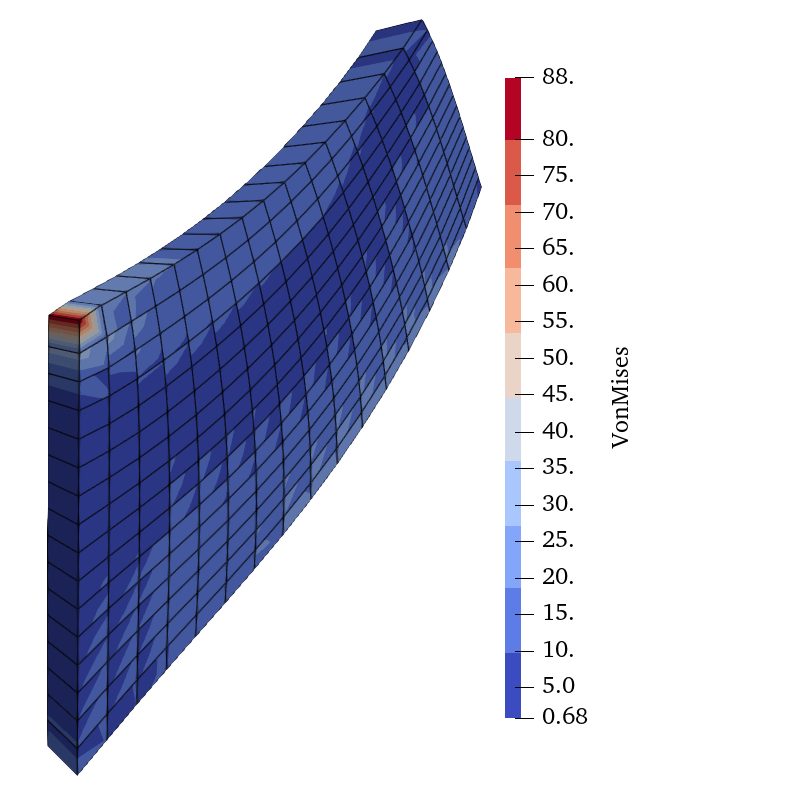
\includegraphics[trim={0 0 4cm 0}, clip, width=0.4\textwidth]{cooks-3d-vonmises-hex-k1.png} \quad 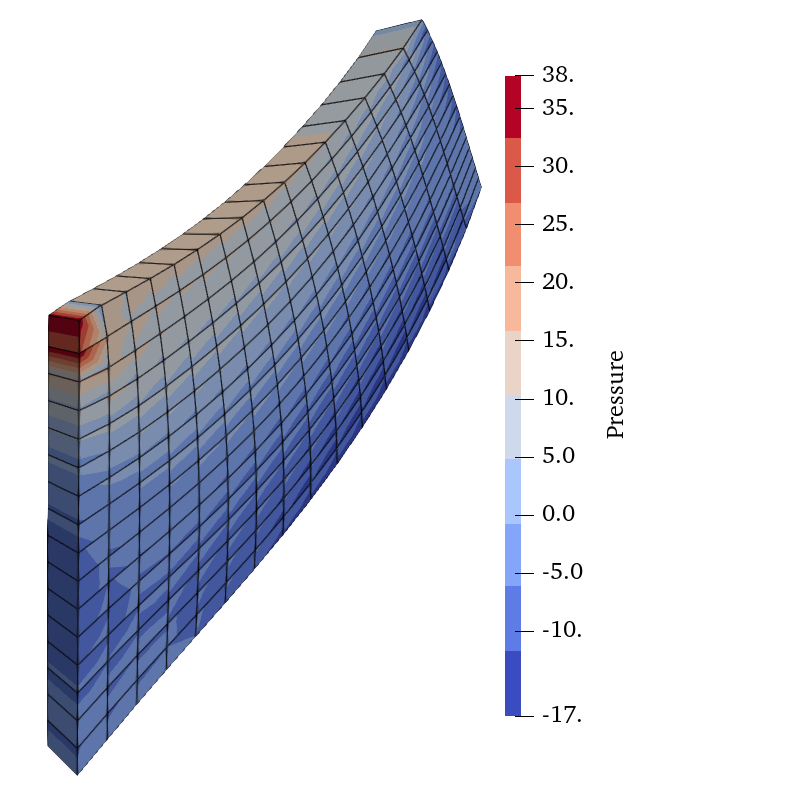
\includegraphics[trim={0 0 4cm 0}, clip, width=0.4\textwidth]{cooks-3d-pressure-hex-k1.png}} \\
	\subfloat[\label{fig:cooks-3d-stress-b}]{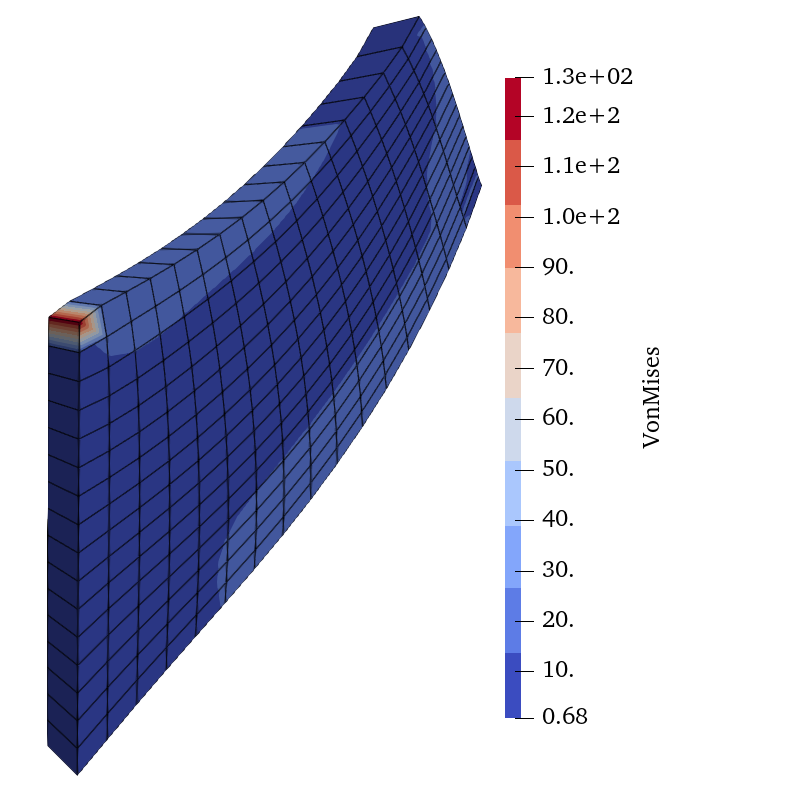
\includegraphics[trim={0 0 4cm 0}, clip, width=0.4\textwidth]{cooks-3d-vonmises-hex-k3.png} \quad 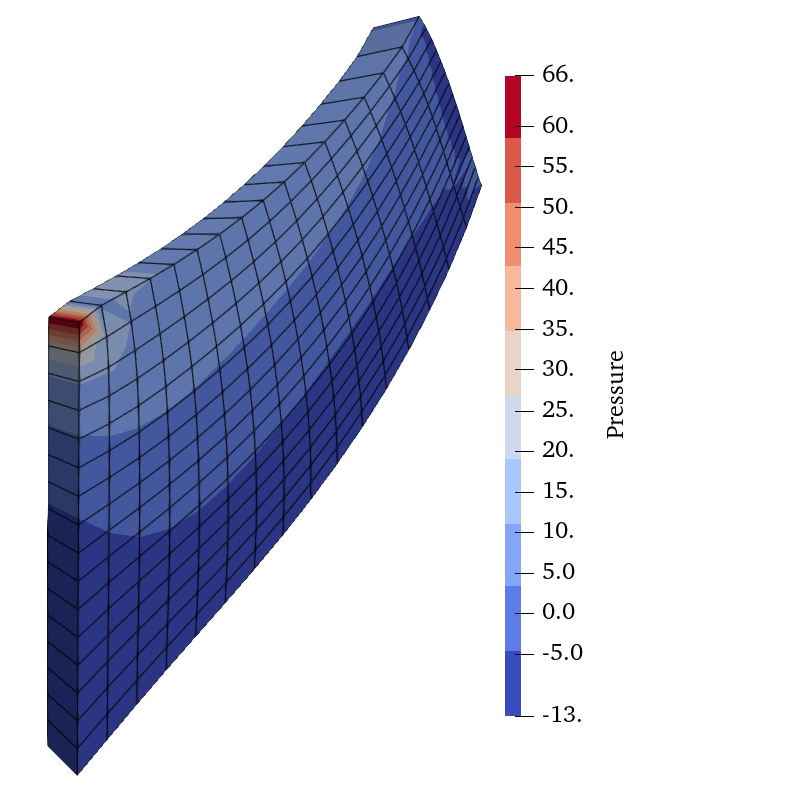
\includegraphics[trim={0 0 4cm 0}, clip, width=0.4\textwidth]{cooks-3d-pressure-hex-k3.png}} \\
	\caption{Cook's membrane. Von Mises stress (at left) and pressure (at right) fields over the deformed configuration using hexahedral meshes with $N_e=16$ for (a) $k=1$ and (b) $k=3$}
	\label{fig:cooks-3d-stress}
\end{figure}

\subsection{Application problem\label{subsec:module}}

To assess the robustness of the proposed method for complex geometries, it is applied to a problem involving the geometry of a structural hull, shown in Figure \ref{fig:module-geometry}. The hull has the following dimensions: $L=1\m$, $r_i=0.345\m$, $r_e=0.390\m$. It is subjected to an internal pressure of $p=10.34$ MPa and fixed in the normal direction of all other faces. The material is assumed to have a linear behavior with a constant Young's modulus of $E=210000$ MPa and a Poisson ratio of $\nu=0.3$. Since the problem is axisymmetric, only one-fourth of the domain is modeled, as shown in Figure \ref{fig:module-geometry}. The results obtained with the proposed formulation are compared with the results obtained using the classical Taylor-Hood formulation.

\begin{figure}[h]
    \centering
    \def\svgwidth{450pt} 
    % 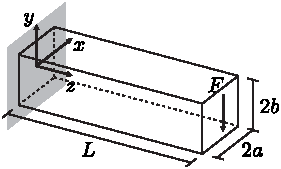
\includegraphics{bishop-beam-geometry.pdf}
    \input{hull-domain.pdf_tex}
    % 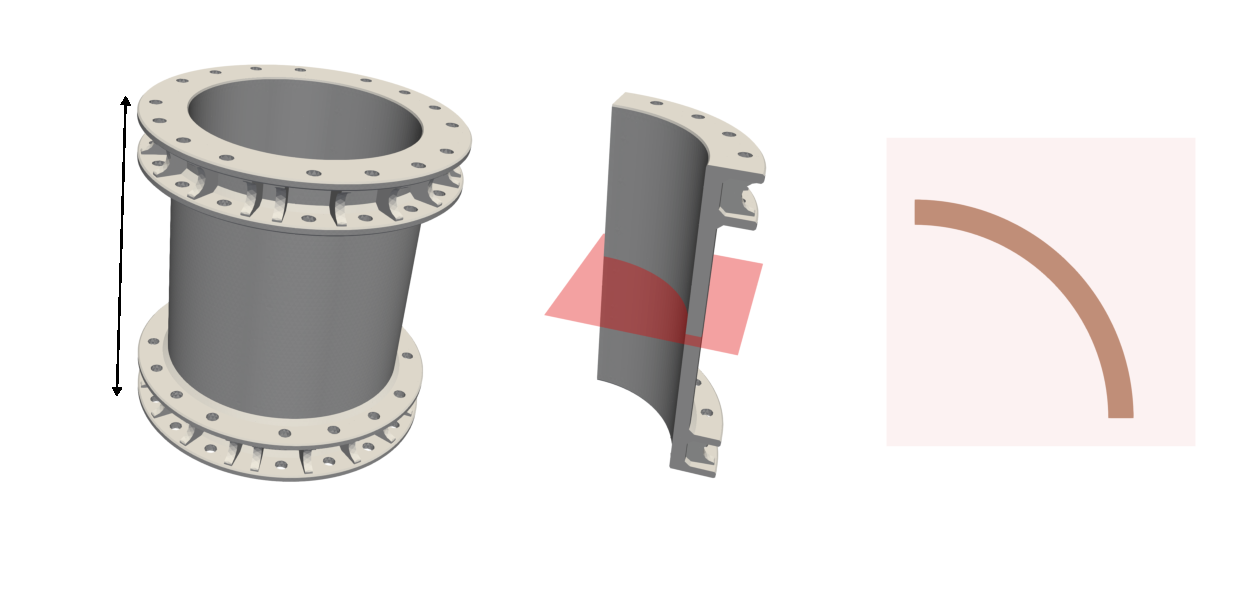
\includegraphics{hull-domain.pdf}
    \caption{Geometry of the structural hull. Only one-fourth of the domain is modeled due to axisymmetry of the domain.}
    \label{fig:module-geometry}
\end{figure}

The problem is solved using an unstructured tetrahedral mesh composed of 68,258 elements, as shown in Figure \ref{fig:module-mesh}. Both the proposed DHM-H(div) and the Taylor-Hood formulations are tested with polynomial degrees $k=2$ and $k=3$, resulting in four different simulations. The results are compared in terms of displacement magnitude, pressure, and Von Mises stresses along a line defined by the points $(259.86, 259.86, 0)$ mm and $(259.86, 259.86, 1000)$ mm. 

The number of degrees of freedom (DOFs) for the DHM-H(div) formulation is 1,336,260 for $k=2$ and 2,440,900 for $k=3$. For the Taylor-Hood formulation, the number of DOFs is 322,447 for $k=2$ and 1,060,639 for $k=3$. The high number of degrees of freedom when using the DHM-H(div) formulation in this problem is due to the use of tetrahedral elements, which increase the number of faces in the mesh. In the DHM-H(div) formulation, the number of degrees of freedom is significantly influenced by the number of element faces in the mesh.

\begin{figure}[h]
	\centering
	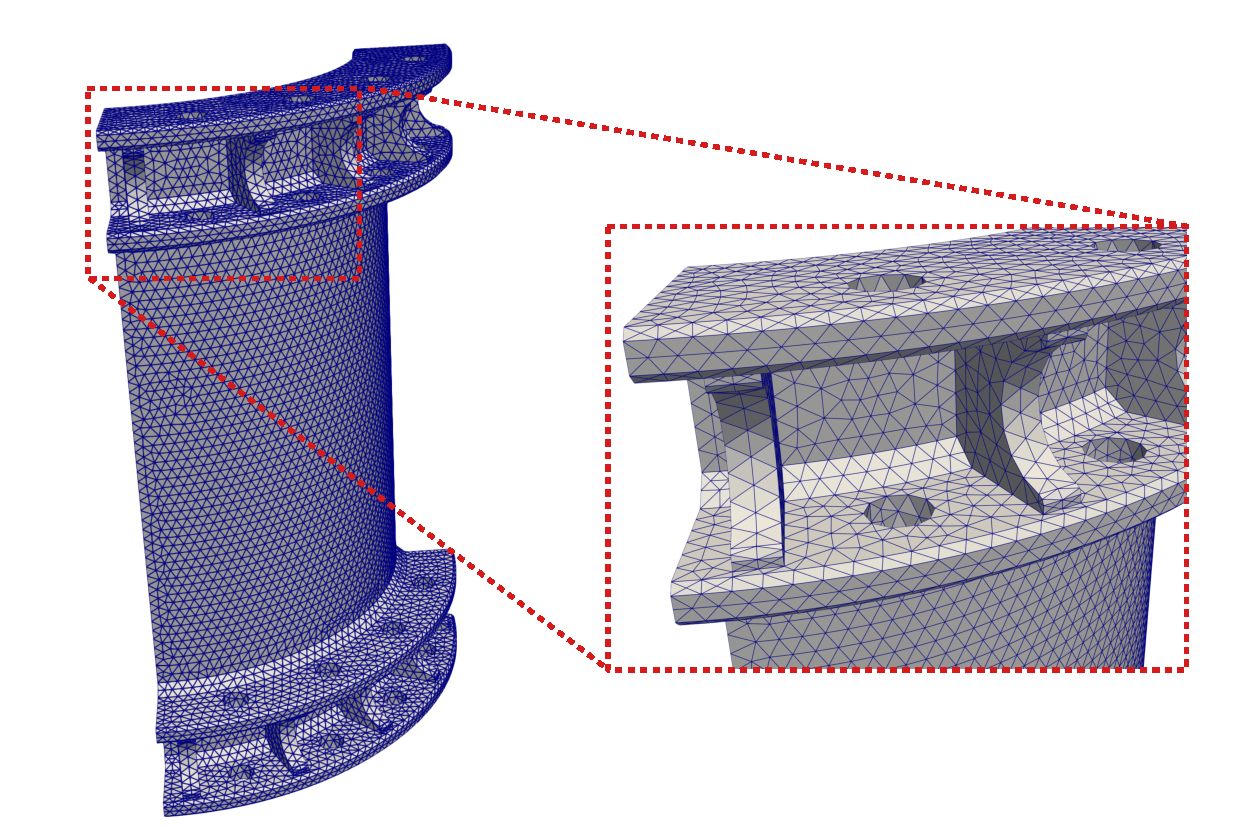
\includegraphics[scale=0.75]{hull-mesh.pdf}
	\caption{Finite element mesh of the structural hull, with a zoom-in highlighting the details of the top region of the domain.}
	\label{fig:module-mesh}
\end{figure}

Figure \ref{fig:module-shapes} shows the structural hull in both undeformed and deformed configurations. Figure \ref{fig:module-shapes-a} presents the undeformed shape with a color map representing the displacement field. Figure \ref{fig:module-shapes-b} illustrates the deformed shape (scaled by 2000 for better visualization) with a color map of the Von Mises stress field, indicating the stress distribution throughout the structure.


\begin{figure}[H]
	\centering
	\subfloat[Undeformed shape with displacement field]{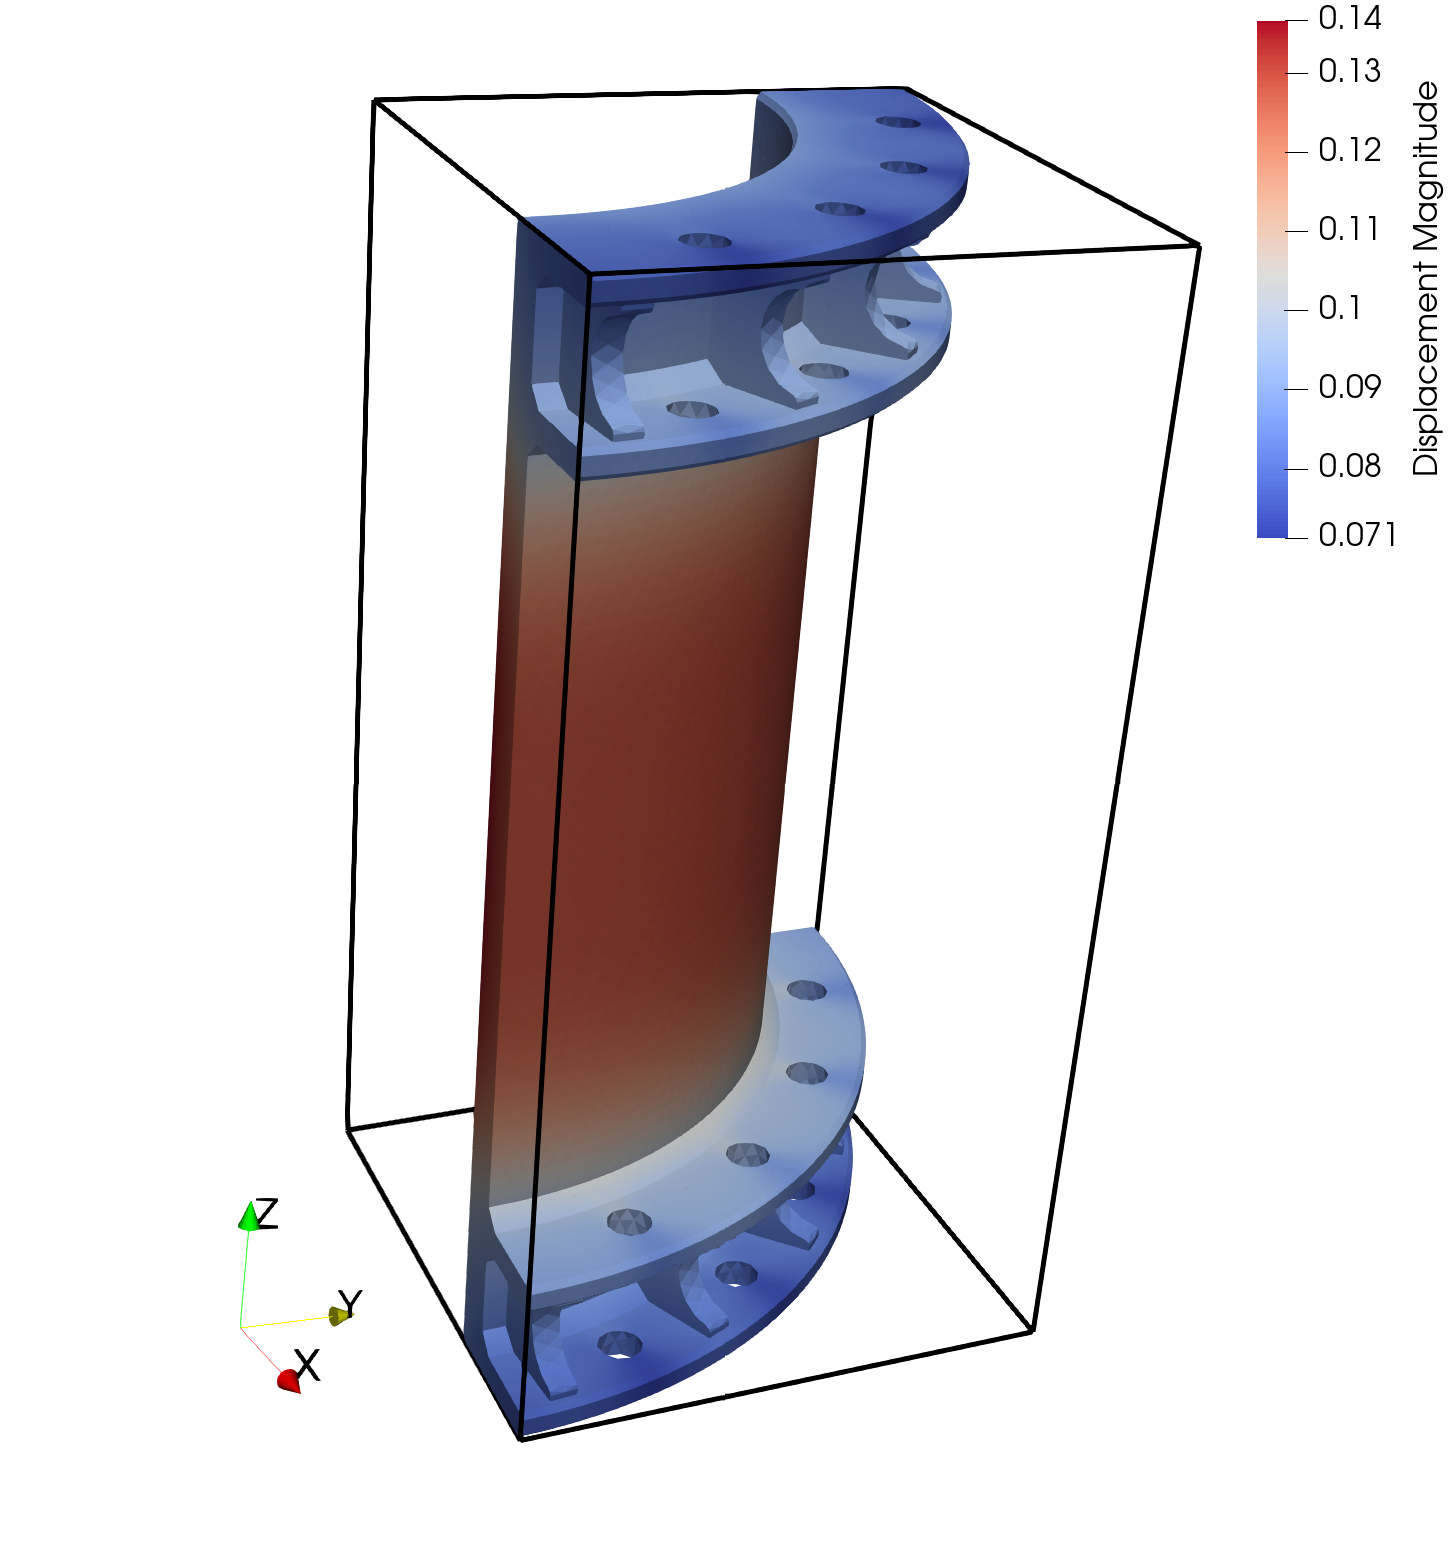
\includegraphics[width=0.45\textwidth]{hull-undeformed.png}\label{fig:module-shapes-a}}
	\hfill
	\subfloat[Deformed shape with Von Mises stress field]{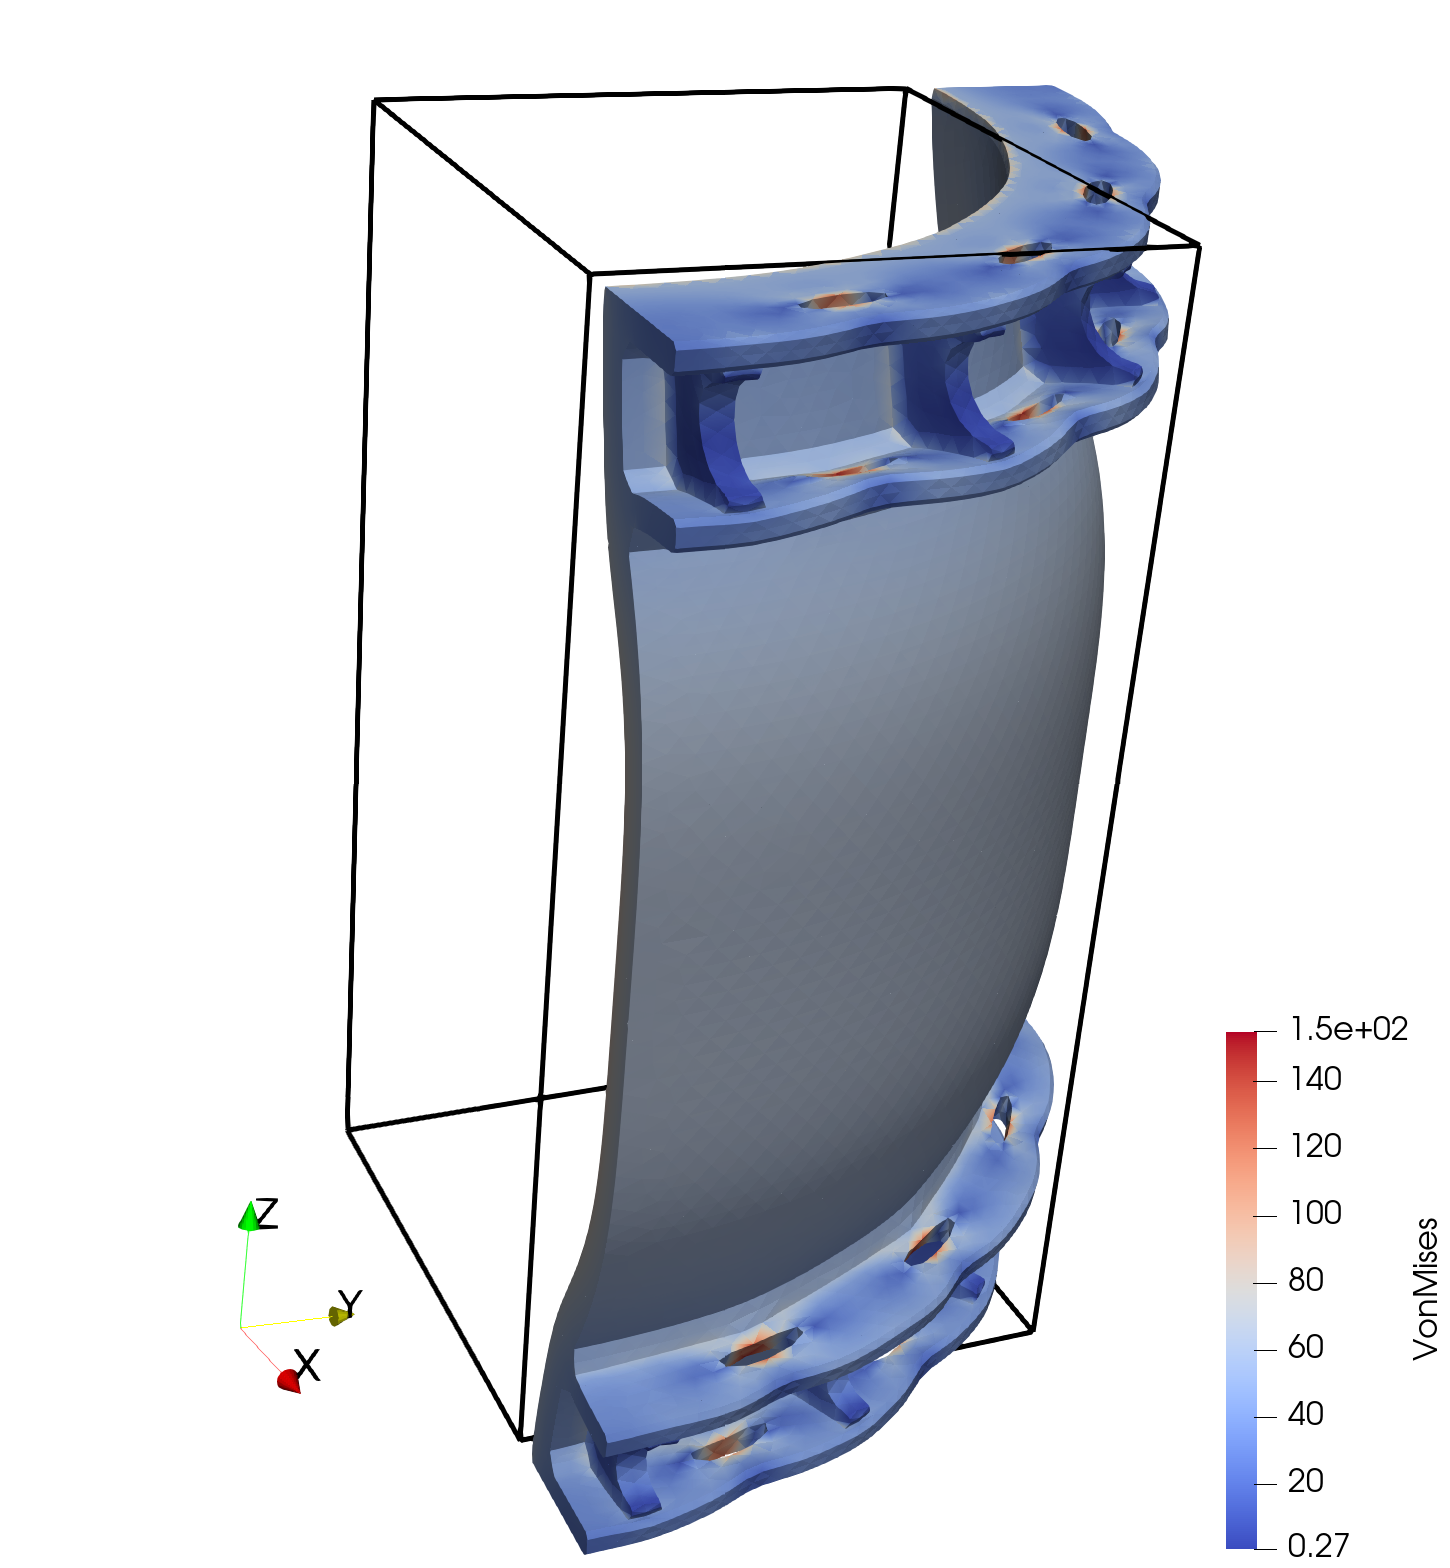
\includegraphics[width=0.45\textwidth]{hull-deformed.png}\label{fig:module-shapes-b}}
	\caption{Structural hull: (a) undeformed shape with displacement field, (b) deformed shape with Von Mises stress field.}
	\label{fig:module-shapes}
\end{figure}

The plots for the displacement magnitude, pressure, and Von Mises stresses along the vertical line through the domain are shown in Figure \ref{fig:module-results}. The results demonstrate that the proposed DHM-H(div) formulation produces results similar to those of the Taylor-Hood formulation for this problem. Smoother solution fields are obtained at the beginning and end of the line for the DHM-H(div) formulation compared to the Taylor-Hood formulation. This can be attributed to the higher amount of degrees of freedom when adopting the DHM-H(div) formulation. 

\begin{figure}[H]
	\centering
	\subfloat[Displacement magnitude]{\includetikz{module_disp}}
	\subfloat[Pressure]{\includetikz{module_pressure}}

	\subfloat[Von Mises Stress]{\includetikz{module_vonmises}}
	\subfloat[Von Mises Stress - Zoom]{\includetikz{module_vonmises_zoom}}
		
	\caption{Comparison of displacement magnitude, pressure, and Von Mises stress distributions along the defined line for the DHM-H(div) and Taylor-Hood formulations with polynomial degrees $k=2$ and $k=3$.\label{fig:module-results}}
	
\end{figure}

\section{Conclusions} \label{sec:conclusions}

In this work, a double hybrid formulation for two and three-dimensional elasticity problems is developed. The approximation space composed of De Rham compatible $H(\text{div})$ functions for normal displacements and $L^2$ functions for the pressure leads to a scheme that is uniformly convergent, independent of the Poisson ratio. It is shown that, using a simple reconstruction of the normal stress, the boundary normal stresses are in local equilibrium.
A second hybridization of the tangential stresses is applied, yielding positive semi-definite element matrices. The resulting global system is symmetric and positive-definite when applied to compressible solids and is a saddle-point problem for incompressible cases, with a single mean pressure per element acting as a Lagrange multiplier to impose the incompressibility constraint.


The formulation is verified through a series of tests. The first one, of a solid mechanics problem with two elasticity coefficients, shows the formulation's ability to capture the correct stress and displacement distributions when compared to the popular Taylor-Hood approximation. The DHM-H(div) formulation is also applied to a cantilever beam subjected to an end shear load, with the results displaying optimal convergence rates of $k+1$ for the displacement and $k$ for the stresses, independent of the Poisson ratio. The formulation was able to capture the correct stress and displacement distributions for the compressible case and a divergence-free displacement field in the case of the incompressibility limit. The Cook's membrane benchmark is also simulated in two and three dimensions, where locking-free solutions are obtained for low-order approximations and good convergence properties are observed when compared against other results from the literature. The simulation of a real-scale structural hull subjected to an internal pressure qualitatively indicates that the proposed method is applicable to complex domain problems.

\bigskip\noindent {\bf Acknowledgments:} The authors thankfully acknowledge the support of ANP - Brazil's National Oil, Natural Gas and Biofuels Agency through the R\&D levy regulation. The acknowledgments are extended to the Center for Petroleum Studies (CEPETRO) and the School of Civil Engineering, Architecture and Urban Planning (FECFAU). G.~Avancini is grateful to Total Energies Brazil through FUNCAMP (processes 23289-2 and 76042-23) and EPIC - Energy Production Innovation Center through FAPESP/Equinor (grant 2023/06981/-5). N.~Shauer (scholarship 2021/03791-5) is grateful to FAPESP - S\~ao Paulo Research Foundation. H.L.~Oliveira thanks the support from FAEPEX PIND grant n. 519.287. P.R.B.~ Devloo acknowledges the Brazilian National Council for Scientific and Technological Development (grants 305823/2017-5 and 309597/2021-8).

%\bibliographystyle{plainnat}
\bibliographystyle{elsarticle-num}
\addcontentsline{toc}{section}{\refname}
\bibliography{%
	references}

\end{document}
